% Hauptdokument fuer Diplomarbeit
% Dank an die Herrn Brunner, Kopetzky und Wurz (2014)

%%%%%%%%%%%%%%%%%%%%%%%%%%%%%%%%%%%%%%%%%%%%%%%%%%
% 1.PACKAGES
%%%%%%%%%%%%%%%%%%%%%%%%%%%%%%%%%%%%%%%%%%%%%%%%%%

% deklariert die Dokumentklasse (einseitig A4 mit 12pkt Schrift)
%\documentclass[12pt,oneside,a4paper]{twdpa}
\documentclass[
fontsize=12pt,
twoside=false,
a4paper,
bibliography=totoc, 		%Literaturverzeichnis ins IV
listof=totoc,				%Abb. & Tab. verz. ins IV
toc=bibliographynumbered, 	%Literaturverzeichnis im IV nummerieren
listof=numbered,			%Abb. & Tab. verz. im IV nummerieren
]{scrreprt}

%Seitenabstände
\usepackage[
a4paper,
includefoot,
includehead,
bottom=1cm, 
top=0.8cm, 
left=25mm, 
right=20mm,
twoside=false,
]{geometry}

\setlength{\headsep}{0.5cm} %Kopfzeilenabstand nach unten
\setlength{\footskip}{0.5cm} %Fußzeilenabstand nach oben
\setlength{\textheight}{24cm} %Höhe der Texte

\usepackage{titlesec} % Textüberschriften anpassen
%Abstände der Überschriften
\titlespacing{\chapter}{0em}{0em}{0em}
\titlespacing{\section}{0em}{1em}{0em}
\titlespacing{\subsection}{0em}{1em}{0em}
\titlespacing{\subsubsection}{0em}{1em}{0em}

%Abstände vor und nach neuen Kapitelüberschriften
\renewcommand*\chapterheadstartvskip{\vspace*{-1cm}}
\renewcommand*\chapterheadendvskip{\vspace*{0cm}}

\usepackage{enumitem} 
% Tabellen über mehrere Seiten

\usepackage{longtable, booktabs}
% passt die Formatierung an die Gegebenheiten des jeweiligen Landes an
\usepackage[ngerman]{babel}
% ermoeglicht die Generierung eines Index mit Hilfe des "\index" Kommandos
\usepackage{makeidx}
% Einbindung von .eps Graphiken
\usepackage{graphicx}
% bindet "schwimmende" Objekte, wie Tabellen und Bilder, ein
\usepackage{float}
% passt eine Bild- und Tabellenüberschrift an (eingerückt, klein und fett)
\usepackage[small,bf]{caption}
% ermöglicht das Anpassen des Seitenlayouts (früher "fancyheadings")
\usepackage{fancyhdr}
% ermöglicht das Verwenden von Umlauten
\usepackage[T1]{fontenc}
\usepackage[latin1]{inputenc}
% ermöglicht das einfügen von EPS (Encapsulated PostScript) Grafiken
\usepackage{graphicx}
%ermöglicht das Erstellen des Bibtex-Literaturverzeichnisses
\usepackage{babelbib}
\usepackage{url} %ordentliche Ausgabe von URLs
%um Seitenanzahl in Fußzeile zu erhalten
\usepackage{totpages}
%Tabellenspalten mit fixer Größe zentrieren
\usepackage{array}
\usepackage{multirow}
%Quellcode ordentlich anzeigen
\usepackage{listings}
%Formatierung des Quellcodes
\usepackage{xcolor}
\lstset{language=PHP, basicstyle = \footnotesize, commentstyle = \color{gray},
    keepspaces = true,
    aboveskip=1.5em,
    abovecaptionskip=0.5em,
    breaklines=true,
    xleftmargin=20pt,
    keywordstyle = \bfseries,
    numbers=left,                   
    numbersep=5pt,                   
    numberstyle=\tiny\color{gray},
    morekeywords={function,return}}
%Damit Tabellen nicht neu positioniert werden (option 'H')
\usepackage{float}
\restylefloat{table}
%Standardschriftart bei Überschriften
\setkomafont{disposition}{\rmfamily}
%rotierte Tabellen
\usepackage{rotating} 
\usepackage{wrapfig}
\usepackage{rotating}
\usepackage[onehalfspacing]{setspace}


%%%%%%%%%%%%%%%%%%%%%%%%%%%%%%%%%%%%%%%%%%%%%%%%%%%%%%%%%%%%%%%%%%%%%%%%%%%
% PDF Attribute
%
\makeatletter
\newif\ifpdfoutput
\@ifundefined{pdfoutput}%
{\let\pdfoutput\@undefined}%
{\ifcase\pdfoutput
  \let\pdfoutput\@undefined
  \else
  \pdfoutputtrue
  \fi
  }%
\makeatother

%Hyperlinks schwarz
\usepackage[bookmarks,colorlinks=true,linkcolor=black,citecolor=black,urlcolor=black]{hyperref}

\let\docext=\pdfext
\pdfpagewidth 210mm \pdfpageheight 297mm
\pdfimageresolution=600 \pdfcompresslevel=1 \pdfinfo{
    /Author (Name)                                               % <<< =========
    /Title (Titel der Diplomarbeit)                              % <<< =========
    /Subject (Diplomarbeit)                                      % <<< =========
    /Keywords (keywords)                                         % <<< =========
}
\pdfcatalog {/PageMode /UseOutlines
    /URI (http://www.htlkrems.ac.at//)
    }
%
%%%%%%%%%%%%%%%%%%%%%%%%%%%%%%%%%%%%%%%%%%%%%%%%%%%%%%%%%%%%%%%%%%%%%%%%%%%


%%%%%%%%%%%%%%%%%%%%%%%%%%%%%%%%%%%%%%%%%%%%%%%%%%
% 2.EINSTELLUNGEN
%%%%%%%%%%%%%%%%%%%%%%%%%%%%%%%%%%%%%%%%%%%%%%%%%%

% Indexgenerierung (Prozessoranweisung)
\makeindex

% setzt den Pfad für Graphiken
\graphicspath{{figures/}}

\setcounter{tocdepth}{3} 
\setcounter{secnumdepth}{3} 

% Zähler der die maximale Nummer von "Floatobjekten" am Beginn einer Seite angibt
\setcounter{topnumber}{2}
% Redefinition: gibt an, wieviel Platz Floatobjekte (Tabellen, Bilder)
% am Beginn einer Seite einnehmen dürfen. (80 Prozent)
\def\topfraction{.8}
% Zähler der die maximale Nummer von "Floatobjekten" am Ende einer Seite angibt
\setcounter{bottomnumber}{2}
% Redefinition: gibt an, wieviel Platz Floatobjekte (Tabellen, Bilder)
% am Beginn einer Seite einnehmen dürfen. (80 Prozent)
\def\bottomfraction{.5}
% maximale Anzahl der Floatobjekte auf einer Seite
\setcounter{totalnumber}{8}
% Redefinition: minimaler Prozentsatz einer Seite der Text auf dem Text stehen muß
\def\textfraction{.2}
% Redefinition: mimimaler Prozentsatz von Floatobjekten die auf einer Floatseite(Seite,
% die nur Tabellen, Bilder enthält) sein müssen
\def\floatpagefraction{.6}
% Einzug des Absatzes auf 0 pt stellen
\setlength{\parindent}{0pt}
% vertikaler Zwischenraum zwischen zwei Absätzen
\setlength{\parskip}{1ex plus 0.5ex minus 0.2ex}
% Teil des "caption" Packages: extra 20pkt links und rechts von einer Beschriftung
\setlength{\captionmargin}{20pt}
%Teil des "float" Packages:
\floatstyle{plain}
% Name eines neuen "schwebenden" Objekts
\floatname{example}{Example}

\newfloat{example}{hbtp}{loe}[chapter]
\floatplacement{figure}{hbtp}
\floatplacement{table}{htbp}

% transformiert "\dollar" zum Dollarzeichen
\newcommand{\dollar}{\char36}	
\newcommand{\source}[1]{\caption*{Quelle: {#1}} }


% Skript fur die Abkürzungen
% neue Umgebung mit einem Argument
\newenvironment{bfscript}[1] {
 % Liste
 \begin{list}
 % keine Eintragsmarkierung
 {}
 {\settowidth{\labelwidth}{\bf #1}
  % Abstand vom Eintrag zum linken Rand auf die Breite des Labels setzen (0, da kein Label)
  \setlength{\leftmargin}{\labelwidth}
  % das Ganze um die Abstand des Label zum Text (auch 0) danach erhöhen
  \addtolength{\leftmargin}{\labelsep}
  % Abstand der Absätze innerhalb eines Eintrages
  \parsep 0.5ex plus 0.2ex minus 0.2ex
  % Abstand der einzelnen Einträge
  \itemsep 0.3ex
  % festlegen des Labels (fett, wenn nötig bis zum Text auffüllen)
  \renewcommand{\makelabel}[1]{\bf ##1\hfill}}}
 {\end{list}
}

%%%%%%%%%%%%%%%%%%%%%%%%%%%%%%%%%%%%%%%%%%%%%%%%%%
% 3.ABTEILUNGEN
%%%%%%%%%%%%%%%%%%%%%%%%%%%%%%%%%%%%%%%%%%%%%%%%%%

% Abteilungsregeln / Vorschriften hier eintragen !
\hyphenation{gleich-zeitig para-meter}

%%%%%%%%%%%%%%%%%%%%%%%%%%%%%%%%%%%%%%%%%%%%%%%%%%
% 4.ANFANG des DOKUMENTES
%%%%%%%%%%%%%%%%%%%%%%%%%%%%%%%%%%%%%%%%%%%%%%%%%%
\begin{document}
% Titelseite einbinden
%
% Titelseite
%
\begin{titlepage}
\begin{minipage}[t]{2.5cm}
\vspace*{-0.3cm}

\includegraphics[width=1.1\textwidth]{figures/krems.pdf}
\end{minipage}
\hfill
\begin{minipage}[t]{9.3cm}
\vspace*{0cm}
\centering
{\large\bf HTBL Krems}\\
\vspace*{0.25cm}
{\small\bf Höhere Lehranstalt für Informationstechnologie}\\
\footnotesize Ausbildungsschwerpunkt System- und Informationstechnik
\vspace*{0.2cm}
\end{minipage}
\hfill
\begin{minipage}[t]{2.5cm}
\vspace*{0.2cm}

\includegraphics[width=1.1\textwidth]{figures/htl.pdf}
\end{minipage}
\hrule

\vspace*{5cm}
\begin{center}
{\Huge \bf DIPLOMARBEIT}\\
\vspace*{2cm}
{\LARGE \bf Webplattform für Rechnungserfassung}
\end{center}
\vspace*{9.1cm}

\begin{minipage}[t]{8cm}
\vspace{0pt}
\begin{flushleft}
\begin{tabbing}
Ausgeführt im Schul\=jahr 2015/16 von:\\[0.4cm]
Florian Mold \>5BHIT-14\\
Michael Vogler \>5BHIT-21
\end{tabbing}
\end{flushleft}
\end{minipage}
\hfill
\begin{minipage}[t]{8cm}
\vspace{0pt}
\begin{flushright}
Betreuer/Betreuerin:\\
\vspace*{0.5cm}
Dipl.-Ing.(FH) Alexander Mestl 
\end{flushright}
\vspace*{1cm}
\end{minipage}

Krems, am 08.04.2016
\vspace*{-10cm}
\end{titlepage}\end{titlepage}

%Römische Seitenzahlen, keine Kopf- und Fußzeile
\pagenumbering{arabic}

%============================================== %
% definiert das Aussehen der Kopf und Fußzeilen
\pagestyle{fancy} %eigener Seitenstil
\fancyhf{} %alle Kopf- und Fußzeilenfelder bereinigen
\chead{
\begin{tabular}{| >{\centering\arraybackslash}m{3.3cm} | p{4.5cm} p{8.1cm}|}
\hline
  \rule{0pt}{4ex} %vertikaler Abstand
  \multirow{4}{*}{
\includegraphics[width=2.87cm]{figures/krems.pdf}} & 
  \multicolumn{2}{c|}{\textbf{HÖHERE TECHNISCHE BUNDES - LEHRANSTALT}} \\[-0.1cm]  & \multicolumn{2}{c|}{\textbf{Krems}} \\
  \cline{2-3} \rule{0pt}{2.8ex} 
   & Abteilung: & \textbf{Informationstechnologie} \\[-0.1cm]
    & Ausbildungsschwerpunkt: & \textbf{System- und Informationstechnik}  \\   
\hline
\end{tabular}
} %
\fancyfoot[R]{Seite \thepage{} von \ref{TotPages}} %Fußzeile Seitenzahl
\renewcommand*{\chapterpagestyle}{fancy} %auch Kapitelseiten haben
\renewcommand{\headrulewidth}{0pt} %Linie unter Kopfzeile entfernen
\setcounter{page}{2} %Pagecounter bei 2 beginnen lassen (wegen Titelblatt)
%============================================== %

%benennt Quellcodelistings von "Listing" auf "Quellcode" um
\renewcommand*\lstlistingname{Quellcode} 

%bindet Vorwort, Erklärung und Zusammenfassungen ein
\vspace*{4cm}

\begin{center}
\textbf{EIDESSTATTLICHE ERKL\"ARUNG}
\end{center}
\begin{center}
\begin{minipage}[c]{9cm}
	Ich erkläre an Eides statt, dass ich die vorliegende Diplomarbeit selbstständig und ohne fremde Hilfe verfasst, andere als die angegebenen Quellen und Hilfsmittel nicht benutzt und die den benutzten Quellen wörtlich und inhaltlich entnommenen Stellen als solche erkenntlich gemacht habe.
\end{minipage}
\end{center}


\vspace{3cm}
\begin{minipage}[t]{8cm}
\vspace{0pt}
\begin{flushleft}
Krems, am 08.04.2016
\vspace*{0.5cm}
\end{flushleft}
\end{minipage}
\hfill
\begin{minipage}[t]{8cm}
\vspace{0pt}
\begin{flushright}
Verfasser / Verfasserinnen:\\
\vspace*{1.5cm}
\hspace*{\fill}\begin{tabular}{@{}l@{}}\hline
\vspace{0.4cm}
\makebox[4cm]{Florian Mold}
\vspace{1.5cm}
\end{tabular}
\vspace*{2cm}
\hspace*{\fill}\begin{tabular}{@{}l@{}}\hline
\makebox[4cm]{Michael Vogler}
\end{tabular}
\end{flushright}
\vspace*{1.5cm}
\end{minipage}5cm}
\end{minipage}
\vspace*{4cm}

\begin{center}
\textbf{GENDER ERKLÄRUNG}
\end{center}
\begin{center}
\begin{minipage}[c]{9cm}
Aus Gründen der besseren Lesbarkeit wird in dieser Diplomarbeit die  Sprachform des generischen Maskulinums angewendet. Es wird an dieser Stelle darauf hingewiesen, dass die ausschließliche   Verwendung der männlichen Form geschlechtsunabhängig verstanden werden soll.   
\end{minipage}
\end{center}
% DIPOLOMARBEITS TABELLEN DEUTSCH ########################
\begin{center}
\textbf{\LARGE DIPLOMARBEIT}

\textbf{DOKUMENTATION}
\end{center}

\begin{tabular}{|p{53mm}|p{110mm}|@{}m{0cm}@{}}
\hline
Namen der \newline Verfasser/innen & Florian Mold \newline Michael Vogler & \\ [0.3cm]
\hline
Jahrgang / Klasse \newline Schuljahr & 5BHIT \newline 2015/16 & \\ [0.3cm]
\hline
Thema der Diplomarbeit & Webplattform für Rechnungserfassung & \\ [0.3cm]
\hline
Kooperationspartner & ELK Fertighaus GmbH & \\ [0.3cm]
\hline
\end{tabular}

\vspace{0.5cm}

\begin{tabular}{|p{53mm}|p{110mm}|@{}m{0cm}@{}}
\hline
Aufgabenstellung & Ziel der Diplomarbeit ist, dass sich die Lieferanten mit ihrer Lieferantennummer bei der Plattform registrieren und warten, bis die Buchhaltung sie freigibt. Danach kann der Lieferant beginnen hochzuladen. Zusätzlich zur Rechnung müssen noch sogenannte Metadaten angegeben werden. Diese beschreiben die Rechnung näher (z.B.: Betrag). Nachdem die Rechnung hochgeladen wurde, erscheint diese in der Buchhaltung. Daraufhin kann ein Buchhalter die Rechnung "holen". Dies bedeutet, dass die Rechnung im PDF-Format mitsamt der Metadaten in Form einer XML-Datei per E-Mail an die automatische Rechnungsverwaltung gesendet wird.  & \\ 
\hline
\end{tabular}

\vspace{0.5cm}

\begin{tabular}{|p{53mm}|p{110mm}|@{}m{0cm}@{}}
\hline
Realisierung & Das System wurde mit der serverseitigen Programmiersprache PHP implementiert. Zusätzlich wurde das Entwicklungsframework Laravel verwendet, um den Entwicklungsprozess zu vereinfachen und zu beschleunigen. Damit die Firma ELK Fertighaus GmbH das System besser in ihre bestehende Struktur integrieren kann, wurde auf eine Oracle-Datenbank gesetzt.  & \\ 
\hline
\end{tabular}

\vspace{0.5cm}

\begin{tabular}{|p{53mm}|p{110mm}|@{}m{0cm}@{}}
\hline
Ergebnisse & Alle Funktionen, die der Auftraggeber vom Projektteam verlangt hat, sind zu seiner Zufriedenheit implementiert. Alle MUSS-Ziele sind in der Anwendung vorhanden und funktional. Auch die optionalen Ziele, nämlich, dass ein Lieferant die Buchhaltung benachrichtigen kann, wenn ein Fehler bei einer seiner Rechnungen aufgetreten ist, wurden implementiert.  & \\
\hline
\end{tabular}
\newpage

\begin{tabular}{|p{53mm}|p{110mm}|@{}m{0cm}@{}}
\hline
Typische Grafik, Foto etc. (mit Erläuterung) & In der untenstehenden Grafik ist die Lieferantenansicht zu sehen. Hier kann eine Rechnung im PDF-Format hochgeladen werden und zusätzlich müssen die Metadaten angegeben werden, bevor der Prozess abgeschlossen werden kann.  \includegraphics[width=310px, height=320px]{upload.png} & \\
\hline
\end{tabular}

\vspace{0.5cm}

\begin{tabular}{|p{53mm}|p{110mm}|@{}m{0cm}@{}}
\hline
Teilnahme an \newline Wettbewerben, \newline Auszeichnungen & Keine & \\
\hline
\end{tabular}

\vspace{0.5cm}

\begin{tabular}{|p{53mm}|p{110mm}|@{}m{0cm}@{}}
\hline
Möglichkeiten der \newline Einsichtnahme in die \newline Arbeit & Bibliothek der HTL Krems & \\ [0.2cm]
\hline
\end{tabular}

\vspace{0.5cm}

\begin{tabular}{|p{5.3cm}|p{5.28cm}|p{5.29cm}|@{}m{0cm}@{}}
\hline
\vspace{-0.6cm}Approbation \newline (Datum / Unterschrift) & \vspace{-1.1cm} Prüfer/in & \vspace{-1.1cm} Abteilungsvorstand / \newline Direktor/in & \\ [1.9cm]
\hline
\end{tabular}ewline Einsichtnahme in die \newline Arbeit & Bibliothek der HTL Krems & \\ [0.2cm]
\hline
\end{tabular}

\vspace{0.5cm}

\begin{tabular}{|p{5.3cm}|p{5.28cm}|p{5.29cm}|@{}m{0cm}@{}}
\hline
\vspace{-0.6cm}Approbation \newline (Datum / Unterschrift) & \vspace{-1.1cm} Prüfer/in & \vspace{-1.1cm} Abteilungsvorstand / \newline Direktor/in & \\ [1.9cm]
\hline
\end{tabular}
% DIPOLOMARBEITS TABELLEN DEUTSCH ########################
\begin{center}
\textbf{\LARGE DIPLOMA THESIS}

\textbf{Documentation}
\end{center}

\begin{tabular}{|p{53mm}|p{110mm}|@{}m{0cm}@{}}
\hline
Authors  & Florian Mold \newline Michael Vogler & \\ [0.3cm]
\hline
Form \newline Academic year & 5BHIT \newline 2015/16 & \\ [0.3cm]
\hline
Topic & Web platform for invoice registration & \\ [0.3cm]
\hline
Co-operation partners & ELK Fertighaus GmbH & \\ [0.3cm]
\hline
\end{tabular}

\vspace{0.5cm}

\begin{tabular}{|p{53mm}|p{110mm}|@{}m{0cm}@{}}
\hline
Assignment of tasks & Target of the diploma thesis is that supplier can register with their suppliernumber. Afterwards they wait until the Accounting unlocks their account. After that they supplier can login into the platform and start to upload bills. Additionally to the bill the supplier has to specify metadatas. They describe the bill in detail (e.g.: suppliernumber, amount, ...). After the bill was uploaded it can be seen by an accounter. Thereupon the accounter can fetch the bill. This means that the bill in PDF-format together with the metadatas in an XML-Document are sent with e-mail to the automatic accounting management. & \\ 
\hline
\end{tabular}

\vspace{0.5cm}

\begin{tabular}{|p{53mm}|p{110mm}|@{}m{0cm}@{}}
\hline
Realization & The system was implemented with the server side programming language PHP. Additionaly the developer framework Laravel was used to simplify the development process. The company ELK Fertighaus GmbH uses only a Oracle Database. So the project team chose it to help them to easier integrate it to their system. & \\
\hline
\end{tabular}

\vspace{0.5cm}

\begin{tabular}{|p{53mm}|p{110mm}|@{}m{0cm}@{}}
\hline
Results & In retrospective all functions, that were required by the contact Person Mister Ferkl were implemented to his satisfaction. All must-goals are available an function well. Also the optional-goals, that a supplier can inform the Accounting, when an error in their bill occured. Another goal was that a accounter can fetch all bills that exist in the system. & \\
\hline
\end{tabular}
\newpage

\begin{tabular}{|p{53mm}|p{110mm}|@{}m{0cm}@{}}
\hline
Illustrative graph, photo (incl. explanation) & In the graphic shown below you can see the supplier-view. There you can upload the bill in PDF-format und add metadatas. \includegraphics[width=310px, height=320px]{upload.png} & \\
\hline
\end{tabular}

\vspace{0.5cm}

\begin{tabular}{|p{53mm}|p{110mm}|@{}m{0cm}@{}}
\hline
Participation in \newline competitions \newline Awards & none & \\ 
\hline
\end{tabular}

\vspace{0.5cm}

\begin{tabular}{|p{53mm}|p{110mm}|@{}m{0cm}@{}}
\hline
Accessibility of \newline diploma thesis & HTL Krems Libary & \\
\hline
\end{tabular}

\vspace{0.5cm}

\begin{tabular}{|p{5.3cm}|p{5.28cm}|p{5.29cm}|@{}m{0cm}@{}}
\hline
\vspace{-0.6cm}Approval \newline (Date / Sign) & \vspace{-1.1cm} Examiner & \vspace{-1.1cm} Head of Department / \newline College & \\ [1.9cm]
\hline
\end{tabular}

%erstellt das Inhaltsverzeichnis
\tableofcontents

\chapter{Präambel}
Dieses Dokument beschreibt die Vorgehensweise bei der Diplomarbeit von Florian Mold sowie Michael Vogler und gibt Rückschluss auf die angewandten Techniken/Umsetzungsschritte. Dabei werden unterschiedliche Bereiche wie das Projektumfeld, die Umsetzung sowie andere ähnliche Aufgabenzweige belichtet.

\section{Team}
Das Projektteam ist für die Durchführung des Projekts hauptverantwortlich.
Die Parteien, bestehend aus Florian Mold und Michael Vogler, sind sich bereits seit längerem bekannt. Die Beteiligten haben im Vorfeld der Diplomarbeit bereits einige schulische Projekte und Referate erfolgreich abgeschlossen. Die Kommunikation der beiden Diplomarbeitspartner war bei jeder Aufgabe stets in Ordnung, weshalb eine Zusammenarbeit bei der Diplomarbeit im Vorhinein geradezu perfekt erschien. Auch privat verstehen sich beide Parteien sehr gut. Im Projekt vertraut jeder stets auf die Fähigkeiten des anderen.

\section{Auftraggeber}
Der Auftraggeber ist diejenige Person, die einen Projektauftrag erteilt und diesen bei der Fertigstellung abnimmt.
Beim Auftraggeber dieser Diplomarbeit handelt es sich um die Firma ELK Fertighaus GmbH. 

\section{Projektbetreuung}
Als Projektbetreuer versteht man den Betreuungslehrer, der dem Team während der Diplomarbeit für projektrelevante Fragen zur Seite steht.
Die Betreuung der Diplomarbeit übernahm Dipl. Ing. Alexander Mestl. Dies war auch die erste Diplomarbeit, die er betreute. Es fanden immer wieder Besprechungen statt, die den Betreuer über den aktuellen Stand der Diplomarbeit informierten. Des Weiteren stand er dem Diplomarbeitsteam immer tatkräftig zur Seite und gab Ratschläge, falls ein Problem bei der Realisierung auftrat.

\section{Abteilungsvorstand}
Der Abteilungsvorstand bestimmt darüber, ob die Diplomarbeit genehmigt wird. Der Abteilungsvorstand, Dipl. Ing Anton Hauleitner stimmte nach dem Ausfüllen des Diplomarbeitsantrags, dem Antrag zu, wodurch die Diplomarbeit als genehmigt galt.

\section{Motivation}
Die Motivation der Diplomarbeit bestand darin, den Rechnungsaustausch der Lieferanten mit der Buchhaltung der Firma ELK Fertighaus GmbH zu optimieren. Vor der Realisierung der Diplomarbeit war die Rechnungsverwaltung mit einem gewaltigen Mehraufwand verbunden, da viele Lieferanten ihre Rechnungen in Briefform übermittelt haben. Daher bestand großer Bedarf nach einem System, das die Rechnungen automatisch an die computerunterstützte Buchhaltung weiterleiten kann und auch die zugehörige XML-Datei mit den Metadaten erzeugen kann. Dabei war auch wichtig, dass der Lieferant keinerlei komplexe Schritte übernehmen muss, die ihn von der Nutzung abschrecken könnten. Es existiert bereits ein System, das folgende Aufgaben übernehmen kann, allerdings ist dieser sehr teuer in der Anschaffung und Wartung. Diese Diplomarbeit stellt daher eine optimale Lösung, die auf die Anforderung der Firma ELK Fertighaus GmbH perfekt zugeschnitten ist, dar. Beide Parteien, nämlich der Auftraggeber sowie das Projektteam, haben aus der Arbeit einen sehr großen persönlichen Nutzen gezogen.

\section{Ausgangssituation}
Die Firma ELK Fertighaus GmbH erhält pro Jahr eine sehr große Anzahl an Eingangsrechnungen in Briefform. Allerdings verwendet die Firma eine elektronische Rechnungserfassung. Daher müssen alle Rechnungen händisch eingescannt werden und mit sogenannten Metadaten, wie zum Beispiel mit dem Betrag oder der Lieferantennummer von der Buchhaltung versehen werden. Dies ist ein sehr bedeutsamer Mehraufwand, der mit dieser Diplomarbeit reduziert werden soll. Danach müssen die Rechnungen im PDF-Format und die Metadaten in XML-Form per E-Mail an die automatische Buchhaltung gesendet werden, damit diese die weiterverarbeiten kann. Einige Lieferanten versenden bereits diese E-Mail, jedoch ist dies nur ein kleiner Bruchteil. Nach Abschluss der Diplomarbeit soll jeder Lieferant die Rechnungen elektronisch an die Firma ELK Fertighaus GmbH senden.

\section{Aufgabenstellung}
Ziel der Diplomarbeit ist, dass sich beim vollständig implementierten System, die Lieferanten mit der Lieferantennummer bei der Plattform registrieren und anschließend warten, bis die Buchhaltung sie freigibt. Danach kann sich der Lieferant anmelden und beginnen, seine Rechnungen im System hochzuladen. Zusätzlich zur Rechnung müssen noch sogenannte Metadaten angegeben werden. Diese beschreiben die Rechnung näher (z.B.: Betrag, Lieferantennummer usw.). Nachdem die Rechnung hochgeladen wurde, erscheint diese auf der Seite der Buchhaltung. Daraufhin kann ein Buchhalter die Rechnung "holen". Dies bedeutet, dass die Rechnung im PDF-Format mitsamt der Metadaten in Form einer XML-Datei per E-Mail an die automatische Rechnungsverwaltung gesendet wird.

\section{Aufgabenteilung}
Die Aufgaben der einzelnen Rollen im Projekt ergeben sich normalerweise aus der Größe des Teams und der Anwendung.

\subsection{Gesamtaufwand}
\begin{table}[!h]
\centering
\caption{Stundenaufwand}\label{tab:stunden}
\begin{tabular}{| c | c |}
\hline
Name & Gesamtaufwand in Stunden (h) \\
\hline
Florian Mold & 177 \\ \hline
Michael Vogler & 176,5\\ \hline
\end{tabular}
\end{table}

\subsection{Florian Mold}
\begin{itemize}
\item Design der Oberflächen
\item hat die \glqq Rechnung holen\grqq -Funktion und die \glqq Benachrichtigungs\grqq-Funktion verwirklicht. 
\item hat den Buchhaltungs- sowie Lieferanten-Login implementiert.
\item hat das Registrieren für Lieferanten umgesetzt.
\item hat \glqq Passwort ändern \grqq , \glqq Passwort vergessen\grqq{} realisiert.
\end{itemize}
Siehe Florian Molds Stundentafel \ref{tab:stundenaufzeichnung}

\subsection{Michael Vogler}
\begin{itemize}
\item hat die Datenbanksynchronisation implementiert
\item hat die \glqq Rechnung hochladen\grqq -Funktion verwirklicht
\item hat das Backend realisiert:
\begin{itemize}
\item Lieferanten verwalten
\item Buchhalter verwalten
\item Passwortkriterien für Buchhalter, Lieferanten und Administrator getrennt bestimmen
\item Standorte der Firma änderbar
\item Währungen, welche die Rechnungen beinhalten dürfen, festlegen
\item Rechnungsarten änderbar
\item die einzelnen E-Mail Adressen für Rechnungssystem, Administrator- und Buchhaltungsbenachrichtigung eintragbar
\end{itemize}
\end{itemize}
Siehe Michael Voglers Stundentafel \ref{tab:stundenaufzeichnung_michael}



\section{Anforderungen}
Die Anforderungen für die Diplomarbeit müssen bereits zu Beginn mit dem Auftraggeber Kunden vereinbart werden. Wenn die genauen Anforderungen des Projekts feststehen, fällt die Realisierung leichter, da die Vorstellung des Kunden nach seinen Wünschen erledigt wird. An den Anforderungen kann man nach Abschluss der Diplomarbeit messen, ob das Endergebnis den Vorstellungen des Kunden entspricht.
Bei dieser Arbeit wurden die Anforderungen mit Herrn Ferkl genauestens ausgearbeitet und schriftlich festgehalten. Die schriftlichen Aufzeichnungen wurden ihm zusätzlich noch vorgelegt, damit er diese noch extra absegnen kann.
Eine Anforderung war zum Beispiel die einfache Bedienung der Anwendung. Die Lieferanten sollten sich nicht um die Erstellung der E-Mail für die Buchhaltung kümmern, sondern einfach nur ihre Rechnungen hochladen können. Aus den Anforderungen konnte man danach die Ziele für die Diplomarbeit ableiten, welche in chronologischer Reihenfolge abzuarbeiten sind. Eine weitere Anforderung war, dass sich an die Coporate Identity der Firma ELK Fertighaus gehalten wird (Logos, Farben vorgegeben).

\section{Zielsetzung}
Die Kommunikation zwischen dem Auftraggeber und dem Auftragnehmer ist für den erfolgreichen Projektabschluss sehr wichtig. Es ist anzuraten, die Erwartungen des Auftraggebers abzustecken, um mögliche Enttäuschungen zu vermeiden. Sind die Ziele vom Projektteam klar definiert, ist es sehr einfach, diese nochmals mit dem Auftraggeber durchzugehen und zu überarbeiten. Die formulierten Ziele sind dem Auftraggeber in Form eines Pflichtenheftes vorzulegen und bei Richtigkeit unterzeichnen zu lassen.
Die relevanten Ziele zur Umsetzung dieses Projekts sind bei Treffen mit Herrn Ferkl erarbeitet und festgehalten worden. Nach der Ausarbeitung der Ziele hat das Projektteam diese in einem Pflichtenheft niedergeschrieben und Herrn Ferkl zu Unterzeichnung vorgelegt. Alle erfassten Ziele, wie diese mit dem Auftraggeber abgehandelt sowie vereinbart und im Pflichtenheft festgehalten wurden, sehen wie folgt aus:

\subsection{Muss-Ziele}
\begin{itemize}
\item Lieferantenplattform 

\begin{itemize}
\item Der Lieferant kann sich mit seiner Lieferantennummer registrieren
und wartet bis er vom Administrator freigeschaltet wird. Nach der
Freischaltung erhält er eine Benachrichtigung per E-Mail. 
\item Nur freigeschaltete Lieferanten können sich auf der Plattform anmelden. 
\item Der Lieferant muss angemeldet sein, um Rechnungen hochladen zu können. 
\item Rechnung hochladen: 

\begin{itemize}
\item Rechnungen im PDF-Format hochladen 
\item Beschlagwortung der Rechnungen, vordefinierte Form muss ausgefüllt
werden. Die Vorgaben für die Beschlagwortung werden von der Firma
ELK an uns genauestens übergeben. 
\end{itemize}
\end{itemize}
\item Buchhaltungsplattform: 

\begin{itemize}
\item Es gibt einen gemeinsamen Buchhaltungsbenutzer, wodurch man das Holen
der Rechnungen nicht für die einzelnen Nutzer mitprotokollieren kann. 
\item Wenn der Buchhaltungsbenutzer angemeldet ist, kann dieser: 

\begin{itemize}
\item Rechnungen herunterladen 
\item Rechnungen einsehen 
\item Rechnungen löschen 
\end{itemize}
\item Pro Rechnung wird eine E-Mail versendet. 
\item E-Mail: 

\begin{itemize}
\item Sie enthält die Rechnung als PDF und die Beschlagwortung als XML-Datei,
welche von Herr Ferkl vorgegeben wird. 
\item Dies wird durch einen von uns generierten Job erledigt. 
\end{itemize}
\end{itemize}
\item Administratoransicht: 

\begin{itemize}
\item Der Administrator kann das Intervall festlegen, wann die Passwörter
geändert werden müssen. 

\begin{itemize}
\item Das Intervall kann für Lieferanten und Buchhalter getrennt festgelegt
werden. 
\end{itemize}
\item Der Administrator kann die Lieferanten freischalten sowie auch sperren. 
\item Nur der Administrator kann den Buchhaltungsbenutzer erstellen. 
\item Der Administrator kann \textbf{\small{}KEINE} Rechnungen holen! 
\item Der Administrator kann Kriterien für Passwörter festlegen. Wenn Passwortkriterien
geändert werden, müssen alle Benutzer bei der nächsten Anmeldung ihr
Passwort ändern.
\end{itemize}
\item Loggen: 

\begin{itemize}
\item Lieferanten: 

\begin{itemize}
\item Wenn ein Lieferant eine Rechnung hochlädt 
\item Wenn ein Lieferant einer Rechnung eine Benachrichtigung hinzufügt. 
\item Ob eine Benachrichtigung hinzugefügt oder eine Rechnung hochgeladen
wird, wird jeweils in einer eigenen Logdatei mitgeschrieben. 
\item Ein Eintrag in der Logdatei sieht so aus: {[}Datum{]}-{[}Uhrzeit{]}-{[}Lieferantnummer{]}-{[}Rechnungsnummer{]} 
\end{itemize}
\item Buchhaltung: 

\begin{itemize}
\item Wann und welche Rechnung gelöscht oder geholt wird. 
\item Beide Fälle, gelöscht oder geholt, werden in einer eigenen Logdatei
gespeichert. 
\item Ein Eintrag im Log sieht so aus: {[}Datum{]}-{[}Uhrzeit{]}-{[}Rechnungsnummer{]} 
\end{itemize}
\item Lieferant freischalten/sperren: 

\begin{itemize}
\item Wenn ein Lieferant freigeschaltet oder gesperrt wird. 
\item Ein Eintrag im Log sieht so aus: {[}Datum{]}-{[}Uhrzeit{]}-{[}Lieferantennummer{]}-{[}freigeschaltet/gesperrt{]} 
\end{itemize}
\end{itemize}
\end{itemize}

\subsection{Optionale Ziele}
\begin{itemize}
\item Lieferantenplattform: 

\begin{itemize}
\item Lieferant sieht, welche seiner Rechnungen noch nicht geholt wurden,
kann aber diese nicht mehr ändern. 
\item Falls der Lieferant eine fehlerhafte Rechnung hochlädt, kann er die
Buchhaltung durch Drücken eines Benachrichtungsbuttons informieren. 

\begin{itemize}
\item Die Benachrichtigung erfolgt via E-Mail. In der E-Mail stehen die
Rechnungsnummer und eine Beschreibung des Fehlers. 
\item In der Datenbank wird die Beschreibung des Fehlers zur Rechnung hinzugespeichert. 
\item Buchhaltungsplattform: Falls eine Beschreibung hinzugefügt wurde,
wird diese gekennzeichnet und die Buchhaltung kann sich die Beschreibung
des Fehlers durchlesen.
\end{itemize}
\end{itemize}
\end{itemize}

\subsection{Nicht-Ziele}
\begin{itemize}
\item Die bestehende automatische Rechnungsverwaltung der Firma ELK soll
nicht verändert werden. 
\item Die Lieferantendatenbank der Firma ELK besteht schon und soll nicht
verändert werden, sondern nur mit unserer Datenbank synchronisiert
werden. 
\item Nach Versenden der E-Mail, welche die Rechnung und die Metadaten enthält,
ist der Aufgabenbereich unserer Diplomarbeit beendet. 
\end{itemize}


\section{Produkt}
Das Produkt, welches als erzeugte Ware beziehungsweise Dienstleistung definiert wird, stellt im Fall der Diplomarbeit eine Webseite dar, mit der es möglich sein soll, dass Lieferanten eine Rechnung hochladen und Lieferanten diese anschließend holen können. Das Projekt soll auf allen Plattformen funktionieren.

\section{Danksagung}
Das Projektteam bedankt sich bei Herrn Professor Wieninger, der im Vorfeld der Diplomarbeit für die Kontaktvermittlung der Diplomarbeitspartner mit dem Vertreter der Firma ELK Fertighaus GmbH, Herrn Ferkl, sorgte. Außerdem geht großer Dank auch an Herrn Ferkl, der diese Diplomarbeit erst möglich machte. Auch half er tatkräftig bei der Realisierung mit, da er Fragen meist sofort und verständlich beantwortete. Für private Treffen opferte er auch seine Freizeit, um noch persönlicher bei der Entwicklung involviert zu sein. Zu guter Letzt möchten wir noch Herrn Professor Mestl bedanken, der diese Diplomarbeit betreute und sich auch immer wieder Zeit nahm um uns bei der Bewerkstelligung zu helfen. Ferner war er auch sehr verständnisvoll, wenn die Ausführung des Projekts nicht optimal lief.


\chapter{Lösungsansätze für die Realisierung}

\section{Technologien}
Im folgenden Kapitel werden die zur Lösung verwendeten Technologien aufgelistet. Es wird näher auf die einzelnen Technologien eingegangen, warum diese verwendet wurden und welche Probleme dabei auftraten.

\subsection{Laravel}
Aufgrund eines Vergleiches vieler Entwicklerframeworks für PHP, wie zum Beispiel Yii2, Symfony2, haben wir uns letztendlich für Laravel entschieden. Hinter Laravel steht eine sehr große und wachsende Community. Die Dokumentation ist sehr umfangreich und erklärt alle Funktionalitäten des Frameworks. Auch viele Anleitungen bezüglich der Entwicklung sind im Internet zu finden.

\subsubsection{Migration}
Migration ist wie eine Versionskontrolle, die es dem Entwicklungsteam erlaubt, das Datenbankschema einfach zu verändern und zu teilen. In Kombination mit dem Laravel-Schema-Builder werden Migrations verwendet, um das Datenbankschema zu entwickeln. Mit der up-Methode in einer Migration-Klasse können neue Spalten zur Datenbank hinzugefügt werden. Durch den Einsatz sogenannter Rollbacks können die Änderungen an der Datenbank auch auf den letzten funktionierenden Stand zurückgesetzt werden. (vgl. \cite{migration})

\subsubsection{Eloquent}
Eloquent ORM ist standardmäßig in Laravel integriert. Jede Tabelle in der Datenbank hat eine zugehörige Klasse, die dazu verwendet, wird mit der Tabelle zu kommunizieren. Diese Modelle erlauben Datenbankabfragen sowie das Einfügen in die Datenbank und Löschen aus der Datenbank. Von Haus aus verwendet Laravel die Mehrzahl der Klasse als Datenbanktabellenname. Zum Beispiel würde bei einer \glqq Flight\grqq{} -Klasse, die Datenbanktabelle \glqq flights\grqq{} verwendet werden. Auch vermutet Laravel, dass jede Tabelle einen Primärschlüssel namens \glqq id\grqq{} besitzt. (vgl. \cite{eloquent}) 

\subsubsection{Blade-Template}
Blade ist eine einfache, aber doch sehr umfangreiche Template-Engine für Laravel. Anders wie andere PHP Template-Engines, verbietet Blade nicht das Verwenden von blanken PHP-Code in den HTML-Seiten. Alle Blade-Views werden in PHP-Code kompiliert und gecached, bis sie modifiziert werden.

Zu Beginn legt man ein Master-Template an, da die meisten Webseiten das gleiche Layout für viele Seiten besitzen. Danach legt man Bereiche fest, an denen die Seiten spezifischen Inhalte geladen werden. Bei einer Seite, die das Master-Template erben soll, muss nur der Name dessen angegeben werden und die spezifisch darzustellenden Daten. (vgl. \cite{blade})

\subsubsection[Artisan-CLI]{Artisan-CLI\footnote{Command Line Interface}}
Artisan ist der Name der in Laravel inkludierten Konsole. Es bietet eine große Anzahl an Kommandos, die sehr hilfreich für das Entwickeln von Anwendungen sind. Zusätzlich zu den bereits vorhandenen Kommandos, kann man auch selbst Befehle definieren. (vgl. \cite{artisan})

\subsubsection[Laravel-Excel]{Laravel-Excel\footnote{http://www.maatwebsite.nl/laravel-excel/docs}}
Laravel-Excel ist eines von vielen Plugins für Laravel, welches den Programmierer beim Auslesen oder Erstellen von CSV- und Excel-Dateien unterstützt. (vgl. \cite{laravelExcel})

Die Unterstützung verfügt über eine sehr gute Dokumentation, wodurch die Installation und die Verwendung relativ einfach sind. Das Plugin ist kostenlos im Internet verfügbar und kann einfach über den Composer (siehe \ref{technologien:composer}) installiert werden.

In dieser Applikation wird das Plugin verwendet, um die Datenbanksynchronisation durchzuführen.

\subsubsection[Laravel-oci8]{Laravel-oci8\footnote{https://github.com/yajra/laravel-oci8}}
Standardmäßig besitzt Laravel keinen Treiber, um auf Oracle-Datenbanken zugreifen zu können. Dies wurde bei der Auswahl des Entwicklerframeworks nicht beachtet, allerdings existieren einige Plugins, wie dieses hier, das die Funktionalität nachträglich implementiert. Über den Composer (siehe \ref{technologien:composer}) kann das Plugin einfach installiert werden. 

Die Erweiterung wurde gewählt, da es eine sehr einfache und leicht verständliche Dokumentation bietet. Des Weiteren kann mit dem Plugin auch die Eloquent-ORM-Technologie aus Laravel verwendet werden, was die Datenbankerstellung erheblich erleichterte. Weiters ist es frei erhältlich.

\subsection{Composer}\label{technologien:composer}
Composer basiert auf PHP und kann als Abhängigskeitsverwalter (Dependency  Manager) bezeichnet werden. Es erlaubt dem Entwickler Bibliotheken zu definieren, von welchen das Projekt abhängt. Außerdem können die Pakete installiert sowie aktualisiert werden. (vgl. \cite{html5})

Das Projektteam hat Composer dazu verwendet, um Laravel und dessen verwendete Erweiterungen zu installieren und aktuell zu halten.

\subsection{Bootstrap}
\begin{quote}
\glqq Bootstrap is the most popular HTML, CSS, and JS framework for developing responsive, mobile first projects on the web.\grqq{} \cite{bootstrap}
\end{quote}
Bootstrap ist ein kostenlos erhältliches Framework, das oft im Bereich Website-Design eingesetzt wird. Es umfasst viele vordefinierte Komponenten, welche man gleich einsetzen oder mit etwas Geschick umschreiben kann.

Das Projektteam verwendete Bootstrap zum Erstellen der Oberfläche. Dies kann man an einigen Komponenten erkennen. Doch hauptsächlich wurde es angewandt, da dieses Framework ein 12-teiliges Gridsystem mitbringt und so die Aufteilung auf den einzelnen Seiten besser gelöst werden kann. Durch diesen Einsatz ist die Applikation auch auf verschieden großen Bildschirmen nutzbar.

\subsection[HTML5]{HTML5\footnote{Hypertext Markup Language}}
\label{technologien:html5}
Unter HTML versteht man eine auf Text basierende Auszeichnungssprache, mit welcher man die Struktur aufbaut. Dokumente mit HTML-Code sind die Grundlage für die Darstellung der Webseiten im www\footnote{World Wide Web}.

Durch HTML ist es möglich, eine Webseite aufzubauen. Diese Webseite kann viele verschiedene Komponenten beinhalten, wie zum Beispiel: Bilder, Text, Videos, Hyperlinks und vieles mehr. (vgl. \cite{html5})

\subsection[CSS]{CSS\footnote{Cascading Style Sheets}}
\label{technologien:css}
CSS wird für HTML- und XML-Dokumente (siehe \ref{technologien:xml}) als Gestaltungs- und Formatierungssprache verwendet. Bei HTML sind bereits einige, vom Browser abhängige, Formatierungen angegeben. Diese können jedoch mithilfe von CSS-Code verändert werden. (vgl. \cite{css})

\subsection{JavaScript}
\label{technologien:javascript}
JavaScript wurde ursprünglich als Erweiterung von HTML und CSS entwickelt und eingesetzt. Es dient dazu, dass die Webseite das macht, was der Entwickler auch wirklich möchte. Das bedeutet, dass mit JavaScript die einzelnen Elemente der Oberfläche verändert werden können. (vgl. \cite{javascript})

In dieser Anwendung wurde JavaScript hauptsächlich für das Verändern der Webseiteninhalte verwendet.

\subsubsection{jQuery}
Die JavaScript-Bibliothek jQuery ist reich an implementierten Features und beeindruckt mit der Arbeitsgeschwindigkeit. Sie unterstützt den Entwickler beim Manipulieren von HTML-Code, beim Animieren und beim Auslösen von Geschehnissen. Überaus praktisch sind die Ajax-Operationen (siehe \ref{technologien:ajax}), denn durch diese können Abfragen usw. im Hintergrund ablaufen. (vgl. \cite{jquery})

In diese Anwendung wurde jQuery eingebunden, da so die Oberfläche nicht immer komplett neu geladen werden musste. Der zweite wichtigere Punkt ist, dass durch die Ajax-Operationen rechenintensivere Operationen im Hintergrund durchgeführt werden können und dennoch die Oberfläche normal verwendet werden kann.

\subsubsection[Ajax]{Ajax\footnote{Asynchronous JavaScript and XML}}
\label{technologien:ajax}
Mit Ajax werden im Hintergrund Daten zwischen Browser und Server übertragen. Das bedeutet, dass HTTP-Requests an den Server abgesendet werden können, während eine Webseite angezeigt wird und es muss nicht die ganze Seite neu geladen werden. (vgl. \cite{ajax})

Im Projekt wurde Ajax oftmals verwendet, um Operationen wie Erstellen oder Bearbeiten usw. durchzuführen und danach eine Fehler- oder Erfolgsmeldung erscheinen zu lassen.

\subsection[Oracle-Datenbank XE]{Oracle Datenbank XE\footnote{Express Edition}}
Die Oracle-Datenbank ist ein relationales Datenbankmanagementsystem des Unternehmens Oracle Corporation. Sie ist eine der vertrauenswürdigsten und meist genutzten relationalen Datenbanken. Das System wird von großen Unternehmen, die Daten über lokale und öffentliche Netzwerke verarbeiten und verwalten, verwendet. (vgl. \cite{oracle})

Das Oracle-Datenbankmanagementsystem kann als Express-Edition (XE) kostenlos genutzt werden. Diese Version ist etwas eingeschränkt, aber für die Entwicklung des Projekts war diese ausreichend. Für Studienzwecke ist die Oracle-Datenbank auf der Herstellerseite frei erhältlich.

Ein Oracle-Datenbanksystem wurde deshalb gewählt, weil die Firma ELK Fertighaus GmbH ausschließlich auf dieses System setzt. Vor der Diplomarbeit bestand nur wenig Kenntnis von Oracle-Datenbanken, weshalb etwas Einarbeitungszeit nötig war. Anfangs traten Probleme bei der Installation der Software auf den Rechnern des Teams auf. 

\subsection[PHP]{PHP\footnote{Hypertext Preprocessor}}
PHP ist eine weitverbreitete Open-Source-Skriptsprache, welche speziell für die Webentwicklung ausgelegt ist. Des Weiteren kann sie direkt in HTML eingebunden werden. Der Unterschied zu zum Beispiel JavaScript besteht darin, dass der PHP-Code auf dem Server ausgeführt wird. Daraus resultiert, dass der Client nur das Ergebnis erhält und nicht weiß, wie der eigentliche Quelltext aussieht. Der wesentliche Vorteil von PHP besteht darin, dass der Einstieg extrem einfach ist, jedoch trotzdem einen riesigen Funktionsumfang bietet. (vgl. \cite{php})

Die Diplomarbeitspartner haben sich einstimmig für die Verwendung von PHP bei der vorwissenschaftlichen Arbeit entschieden. Die Programmierung und der Einsatz der Programmiersprache war den Mitgliedern aus einigen schulischen Projekten bereits sehr vertraut. Auch findet sich im Internet eine sehr detaillierte Dokumentation und die meisten Problemstellungen wurden bereits in diversen Foren behandelt. Zudem bietet PHP auch eine Reihe sogenannter Frameworks, die die Entwicklung vereinfachen sollen. Die Spanne reicht hier vom Enterprise-Einsatz bis hin zur schnellen Anwendungsentwicklung. Die Programmiersprache kommuniziert hauptsächlich über HTTP, weshalb es die erste Wahl für Webprojekte ist.

\subsection[XML]{XML\footnote{Extensible Markup Language}}
\label{technologien:xml}
Diese Technologie dient dem Austausch sowie der Beschreibung von komplexen Datenstrukturen. Es handelt sich um eine Auszeichnungssprache, mit der andere Auszeichungssprachen (HTML) um Informationen erweitert werden können. Der Inhalt einer XML-Datei ist auch für den Menschen les- und interpretierbar. In seinem grundsätzlichen Aufbau ähnelt XML dem HTML-Standard. Allerdings bietet XML die Möglichkeit Elemente, die weitere Elemente oder Attribute beinhalten können, selbst zu definieren. Mit XML wird der Austausch von Daten zwischen verschiedenen Systemen (Unternehmenskommunikation) um ein Vielfaches erleichtert. (vgl. \cite{xml})

Für die Diplomarbeit wird XML verwendet, um die Metadaten in einer Datei zu verpacken, die für das computerunterstützte Buchhaltungssystem der Firma ELK Fertighaus GmbH interpretierbar ist. Die Richtigkeit der Werte in der Datei konnte durch die einfache Lesbarkeit von XML-Tags ohne Probleme überprüft werden.
\newpage
\subsection[LATEX]{LATEX\footnote{Lamport TeX}}
\begin{quote}
\glqq LaTeX ist ein Textsatzsystem. Bei LaTeX verfasst man ein Eingabedokument in reinem Text in einem Text-Editor. Dabei schreibt man inhaltliche Fließtexte und spezielle LaTeX-Befehle. Daraus wird ein formatiertes Ausgabedokument (beispielsweise PDF) erzeugt.  \cite{latex}
\end{quote}

Das Projektteam hat Latex gewählt, da so beide Parteien unabhängig voneinander ihr schriftlichen Teil verfassen können. Zum Abschluss der schriftlichen Arbeit müssen nur noch die Dateien in das Hauptdokument eingebunden werden und Latex erstellt die notwendigen Verzeichnisse, wie zum Beispiel das Abbildungsverzeichnis, automatisch für alle Einträge. Bei Latex kann man sich auch auf den Inhalt der Projektarbeit konzentrieren und muss sich nicht mit der aufwendigen Formatierung des Dokuments abmühen, da die Darstellung alleinig das Verarbeitungsprogramm übernimmt. Des Weiteren ist die Technologie ohne Lizenz verwendbar und auch gratis.

\subsection{Cronjob}
Unter Cronjob versteht man einen unter Linux auszuführenden Dienst, welcher Skripte und Programme automatisch zu einer gewissen Zeit ausführt. Die einzelnen Befehle werden in der crontab-Tabelle gespeichert.

Ein Eintrag in dieser Tabelle besteht aus fünf bis sechs Spalten. Am Beginn steht die Zeitangabe (Minute, Stunde, Tag, Monat, Wochentag), darauf folgt der Benutzername, welcher den Befehl ausführt und am Ende wird der zu kompilierende Befehl angegeben. Unterteilt werden die Spalten durch Leerzeichen oder Tabulatoren. (vgl. \cite{cronjob})

Das Team setzte einen Cronjob ein, um die Datenbanksynchronisation und die Datenbanksicherung durchzuführen. Der Cronjob, den die Anwendung benötigt, wird jede Minute ausgeführt und mittels Laravel der Zeitpunkt zur Durchführung der einzelnen Funktionen bestimmt.usgeführt und mittels Laravel der Zeitpunkt zur Durchführung der einzelnen Funktionen bestimmt.
\section{Entwicklungsumgebung}
Im folgenden Abschnitt werden die verschiedenen Entwicklungsumgebungen und ihre Funktionalitäten näher beschrieben.

\subsection{JetBrains PhpStorm}
PhpStorm ist die IDE\footnote{Integrierte Entwicklungsumgebung} für die Programmiersprache PHP der Firma JetBrains. Die IDE punktet durch ihre Schnelligkeit und eine große Anzahl an Funktionen, die von Haus aus mitgeliefert werden, wie zum Beispiel Syntax-Highlighting, intelligente Strukturverbesserung des Quellcodes usw. Das Produkt wird zudem ständig aktualisiert und kann durch zahlreiche Erweiterungen noch weiter verbessert werden. (vgl. \cite{phpstorm})  

Für detailliertere Informationen siehe Hersteller-Webseite.\footnote{\url{https://www.jetbrains.com/phpstorm/}} \\ 

Zur Verwendung benötigt man allerdings eine Lizenz, die das Diplomarbeitsteam durch den Besuch an der HTL-Krems für ein Jahr kostenlos erhalten hat. 

Dadurch, dass das Projektteam bereits einige Erfahrungen mit PhpStorm bei schulischen Projekten gesammelt hat, war der Einsatz der Software bei dieser Projektarbeit im Vorhinein bereits klar. Die Entwicklung gestaltet sich durch die verschiedenen Hilfen, die die IDE bietet sehr einfach und intuitiv. Fehler, die in einfachen Texteditoren auftreten, wie zum Beispiel, dass Variablen noch nicht gesetzt wurden, oder sich deren Name bei der Verwendung unterscheidet, traten mithilfe PhpStorms bei der Diplomarbeit nicht auf, was einen immensen Zeitgewinn zur Folge hatte.


\subsection{Oracle-SQL-Developer}
Oracle-SQL-Developer ist eine grafische Version von SQL-Plus, die Datenbank-Entwicklern eine Möglichkeit gibt, grundlegende Aufgaben einfach zu erledigen. Diese können Datenbankobjekte betrachten, ansehen, bearbeiten und löschen. Des Weiteren kann man SQL-Abfragen an eine Datenbank senden. Außerdem besitzt die Software, die Möglichkeit Daten zu exportieren bzw. zu importieren ,wie zum Beispiel CSV- oder Excel-Dateien. Verbindungen zu einer Datenbank lassen sich mit einer Standardauthentifizierung (Benutzername, Passwort) aufbauen. Einmal verbunden, kann man Operationen in der Datenbank durchführen. (vgl. \cite{sqldeveloper})

Für detailliertere Informationen siehe Hersteller-Webseite.\footnote{\url{http://www.oracle.com/technetwork/developer-tools/sql-developer/overview/index-097090.html}} \\ 

Der Grund für den Einsatz in der Projektarbeit ist, dass die Software (nach einer Registrierung) frei erhältlich ist. Außerdem ist das Programm sehr einfach in der Handhabung und bietet einwn sehr großen Funktionsumfang, von der die Entwicklung sehr profitierte.



\subsection{XAMPP} 
Das Programm XAMPP stellt eine Sammlung verschiedenster freier Software dar. Es bietet eine einfache Installation und Konfiguration des Webservers Apache mit der relationalen Datenbank MariaDB und den Skript-Sprachen Perl und PHP. Das X im Namen der Software steht für die unterschiedlichen Betriebssystemen, auf denen es verfügbar ist (Linux, Microsoft Windows, Mac OS X, Solaris). Zusätzlich sind in der Sammlung noch andere nützliche Werkzeuge enthalten, wie ein FTP-Server, FileZilla, Mail-Server, phpMyAdmin, OpenSSL und Webalizer. Ziel des XAMPP-Projekts ist eine möglichst einfache Installation von Server-Werkzeugen zu bieten, die ansonsten lange konfiguriert werden müssten. (vgl. \cite{xampp})

Für detailliertere Informationen siehe Hersteller-Webseite.\footnote{\url{https://www.apachefriends.org/de/index.html}} \\ 

Zur Realisierung des Projekts wurde allerdings nur der Apache-Server und die Skript-Sprache PHP eingesetzt. XAMPP wurde verwendet, da es eine schnell einzurichtende lokale Entwicklungsumgebung bietet. Direkt nach der Installation kann mit der Entwicklung von Web-Applikationen begonnen werden. Der Apache-Server musste allerdings erweitert werden, damit er die Oracle-Datenbank abfragen und verarbeiten kann. Apache besitzt eine freie Software-Lizenz der Apache-Software-Foundation.


\subsection{Google Chrome}
Google Chrome ist ein Webbrowser des amerikanischen Unternehmens Google Inc. 
Das Projektteam hat den Browser hauptsächlich für die Entwicklung gewählt, da er so eine große Verbreitung findet und deshalb die Weboberfläche darauf angepasst werden muss. Auch bietet Google Chrome großartige Entwicklertools, die das Manipulieren des Quelltexts direkt auf der Webseite zulassen. Auch verfügt das Programm über eine Konsole, die über aufgetretene Fehler, wie zum Beispiel über eine fehlende CSS-Datei oder Fehler bei einer JavaScript-Methode informiert.

Für detailliertere Informationen siehe Hersteller-Webseite.\footnote{\url{https://www.google.de/chrome/browser/desktop/}} \\ 

\subsection{Mozilla Firefox}
Mozilla Firefox ist ein freier Webbrowser des Entwicklers Mozilla Corporation. 
Zur Entwicklung wurde ebenso Mozilla Firefox gewählt, da er von vielen Anwendern eingesetzt wird. Auch bietet er ähnliche hilfreiche Entwicklerwerkzeuge wie Google Chrome. Zudem kann man die Webseite mit einem nützlichen Tool untersuchen, dass den Aufbau der Seite in einer 3D-Ansicht offenlegt. Dies wird genutzt, um herauszufinden, ob vielleicht ein Element zu breit ist, wenn die Seite nicht wie gewünscht dargestellt wird.

Für detailliertere Informationen siehe Hersteller-Webseite.\footnote{\url{https://www.mozilla.org/de/firefox/new/}} \\ 

\subsection{Dropbox}
Dropbox ist eine freie Software, die Dateien in der Cloud (Speicherplatz im Internet) sichert. Wenn eine Datei auf Dropbox hochgeladen wurde, kann man sie von jedem internetfähigen Gerät abrufen. In der Standard-Version steht ausreichend Speicher zur Verfügung.

Das Projektteam hat Dropbox zum Dateiaustausch sowie zum Absichern der relevanten Dateien genutzt. Allerdings traten dabei auch einige Probleme auf, da des Öfteren Dateien in \glqq Konflikt\grqq{} standen, was bedeutet, dass beide Projektpartner die selbe Datei bearbeitet und gespeichert haben. Dies führte zu Dateien, die doppelt vorhanden waren. Dadurch mussten die Dateien analysiert werden, um die aktuelle zu finden. Auch sind einige Dateien bei der Entwicklung verloren gegangen, was mit Mehraufwand verbunden war, da diese erneut geschrieben werden mussten.

Für detailliertere Informationen siehe Hersteller-Webseite\footnote{\url{https://www.dropbox.com/de/}}. \\

\subsection{Texmaker}
Texmaker ist ein frei erhältlicher, moderner und auf vielen Plattformen erhältlicher Latex-Editor. Es beinhaltet viele Funktionalitäten (Rechtschreibprüfung, Autovervollständigung, usw.), die benötigt werden, um professionell Dokumente zu erstellen. (vgl. \cite{texmaker})

Aufgrunddessen, dass das Projektteam zuvor eine Einführung zu dieser Anwendung erhalten hat und daher bereits einige hilfreiche Funktionen bekannt waren, sowie durch die automatische Codevervollständigung wurde das Entwerfen des Dokuments um einiges beschleunigt.

Für detailliertere Informationen siehe Hersteller-Webseite.\footnote{\url{http://www.xm1math.net/texmaker/}} \\


\section{Datenbankmodell}

\subsection{Oracle-SQL-Developer-Data-Modeler}
Der Oracle-SQL-Developer-Data-Modeler ist ein Tool mit einer graphischen Oberfläche und kann kostenlos im Web erworben werden. Es unterstützt die Benutzer einer Oracle-Datenbank beim Erstellen und Bearbeiten der verschiedensten Datenbankmodelle. Der Modeler kann am eigenen Computer laufen, aber auch auf eine Datenbank in einer Cloud zugreifen. (vgl. \cite{modeler})

Das Team verwendete den Oracle-SQL-Developer-Data-Modeler nur, weil es keine anderen Alternativen gab. Es kamen einige Problem, welche viel Zeit in Anspruch nahmen, zum Vorschein, doch es wurden alle gelöst. Das Erstellen der Datenbank war eine große Herausforderung, da die Oberfläche kompliziert gestaltet ist. Außerdem gibt es keine gute Übersichtsansicht der Tabellen. Bei der bestehenden Übersicht sind die Relationen zwischen den Tabellen schwer ablesbar.

Die Übersicht unserer Datenbank haben wir mit der \glqq MySQL-Workbench\grqq{} von der Oracle-Corporation erstellt. Auf dieser Ansicht sind die Relationen schön erkennbar und übersichtlich gestaltet.

\subsection{Tabellen}
Im folgenden Abschnitt werden die Tabellen der Datenbank näher beschrieben. In jeder Tabelle existieren die Felder \glqq created\_at\grqq{} und \glqq updated\_at\grqq{}. Diese werden von Laravel bei der Datenbankerzeugung automatisch generiert und beschreiben, wann der Eintrag erstellt und zuletzt verändert wurde.

\subsubsection{bills}
Die Tabelle dient dazu, die Rechnungen, die von den Lieferanten hochgeladen werden, zu speichern. In dieser wird der Pfad der PDF-Datei sowie das Datum der Rechnung gespeichert. Des Weiteren speichert die Anwendung den Betrag und den Steuerbetrag. Falls der Lieferant der Rechnung eine Benachrichtigung hinzufügt, wird diese ebenfalls zum Rechnungseintrag hinzugefügt. Außerdem wird der Status der Rechnung (gelöscht, geholt, neu) gespeichert. Es existieren Fremdschlüssel-Beziehungen zu der Rechnungsarten-, Währungen-, Firmen- und Lieferanten-Tabelle.
\subsubsection{companies}
In der Firmen-Tabelle werden die Standorte der Firma ELK Fertighaus GmbH gespeichert. Es gibt ein Feld, das die Kürzel der verschiedenen Standorte speichert (001, 002). Dies wird benötigt, um später die XML-Datei bei dem Rechnung holen zu erstellen.
\subsubsection{currencies}
In der Währungen-Tabelle werden die verfügbaren Währungen für die Rechnungen gespeichert. Auch hier existiert ein Feld, das die Abkürzungen der Währungen speichert (EUR, GBP). Dies wird ebenfalls benötigt um die XML-Datei zu generieren.
\subsubsection{billtypes}
In der Rechnungsarten-Tabelle werden die verschiedenen Rechnungstypen (Rechnung, Gutschrift) gespeichert. Das Kürzel-Feld beinhaltet die Abkürzungen der Rechnungsarten (R, G). Diese Tabelle wird ebenfalls zum Erstellen der XML-Datei benötigt.
\subsubsection{users}
In dieser Tabelle werden alle Benutzer der Anwendung gespeichert. Es wird der Benutzername, die E-Mail sowie das Passwort gespeichert. Ebenso wird gespeichert, ob der Benutzer sein Passwort beim Anmelden ändern muss. Zudem werden noch die Berechtigungen der einzelnen Benutzer gesichert (Lieferant, Buchhalter, Administrator). Zudem erhält es ein Feld, das angibt, ob der Benutzer gesperrt ist, daher kann er sich nicht anmelden.
\subsubsection{suppliers}
In der Lieferanten-Tabelle werden die Lieferanten-Informationen gespeichert. Die Informationen der Tabelle werden aus einer Excel-Tabelle, die von der Firma ELK Fertighaus zur Verfügung gestellt wird, gespeist. Es existiert eine Fremdschlüssel-Beziehung zu der Users-Tabelle. Die Tabelle erfüllt den Zweck, dass die Lieferanten-Daten, die einem Benutzer zugehörig sind, auch richtig in der XML-Datei verwendet werden.
\subsubsection{emails}
In dieser Tabelle werden die verwendeten E-Mails und deren Verwendungszweck gespeichert. Es existieren E-Mails zum Versenden und zum Empfangen von Nachrichten.
\newpage 
\subsubsection{password\_criterias}
Diese Tabelle beinhaltet die Passwortkriterien für jede einzelne Benutzergruppe (Administrator, Buchhalter, Lieferant). Es ist festlegbar, ob das Passwort Sonderzeichen, Zahlen, minimale Zeichenanzahl, Groß- und Kleinschreibung enthalten muss. Des Weiteren existiert ein Feld, in welchem Intervall das Passwort geändert werden muss (z.B.: jede Woche).

\subsubsection{jobs}
In dieser Tabelle werden die Jobs gespeichert, die von der Anwendung generiert werden. Zum Beispiel E-Mails. Beim Aktivieren des zugehörigen Artisan-CLI-Befehls werden die Einträge der Tabelle abgearbeitet und anschließend entfernt.
\subsubsection{failed\_jobs}
In dieser Tabelle werden die fehlgeschlagenen Jobs gespeichert, zum Beispiel eine XML-Datei, die versendet werden soll, existiert nicht mehr. Wenn ein Job in der Jobs-Tabelle nicht abgearbeitet werden kann, wird er in diese Tabelle verschoben und zu einem späteren Zeitpunkt abgearbeitet. Damit wird der Geschwindigkeit der Anwendung kein Abbruch getan.

\begin{sidewaysfigure}
\centering
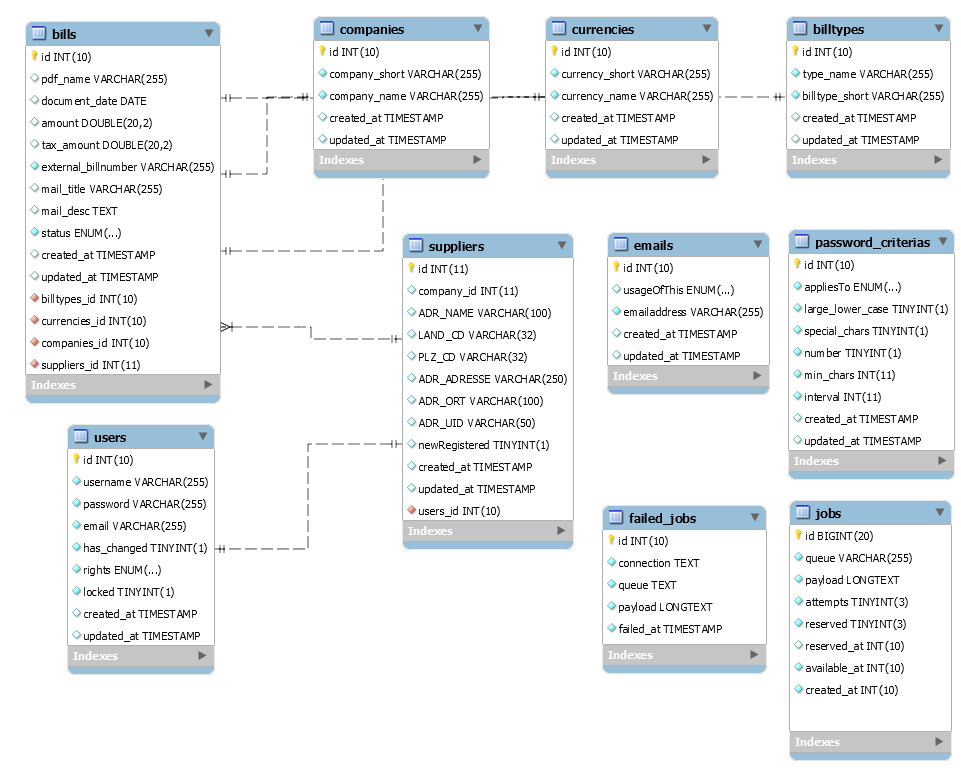
\includegraphics[scale=0.9]{figures/datenbank.PNG}
\caption{ER-Modell der Datenbank}
\label{fig:ermodell} 
\end{sidewaysfigure}
\chapter{Dokumentation der Implementierung}
Im folgenden Kapitel wird eine detaillierte Beschreibung der wichtigen Funktionen geliefert. Zudem sind Code-Ausschnitte sowie Screenshots der einzelnen Funktionen zur besseren Verständlichkeit vorhanden. 

\section{Registrieren}
Das Fenster, um sich als Lieferant zu registrieren, kann über den Lieferanten-Login aufgerufen werden. Diese Funktion wird ausschließlich von Lieferanten in Anspruch genommen, die ihre zukünftigen Rechnungen auf die Plattform hochladen wollen. Beim Registrieren kann der Lieferant einen Benutzernamen, eine E-Mail-Adresse und ein Passwort, das den vorgeschriebenen Kriterien entspricht, eintragen. Zusätzlich muss er seine ELK Fertighaus GmbH interne Lieferantennummer angeben, um die Registrierung abschließen zu können. Diese Nummer kann er aus einer Liste auswählen, in der die Bezeichnung des Lieferanten zusätzlich zu der Lieferantennummer angegeben ist. Bei der Registrierung wird überprüft, ob die Form komplett ausgefüllt wurde, ob die beiden eingegebenen Passwörter übereinstimmen und infolgedessen, ob das Passwort den Passwortkriterien aus der Datenbank entspricht. Wenn ein Fehler bei der Registrierung auftritt, wird der Benutzer mit einer entsprechenden Fehlermeldung versorgt. Nach Abschluss der Registrierung erhält der Lieferant eine E-Mail, die bestätigt, dass er sich erfolgreich registriert hat. Weiters wird ein neuer Benutzer in der Datenbank angelegt und die Benutzer-ID dem zugehörigen Lieferanten zugewiesen. Das eingegebene Passwort wird mit einer Laravel internen Funktion\footnote{\url{https://laravel.com/docs/5.2/hashing}} verschlüsselt und so in die Datenbank geschrieben. Allerdings kann der Lieferant sich zu diesem Zeitpunkt noch nicht registrieren, da die Buchhaltung seinen Benutzer erst freischalten muss.
\newpage
Unten sehen Sie einen Ausschnitt aus der Registrier-Methode. Die Methode erstellt den Benutzer und prüft, ob die Lieferantennummer existiert. Wenn diese existiert, wird dem Lieferanten die zugehörige Benutzer-ID zugewiesen. Abschließend wird noch eine E-Mail an den Lieferanten versendet.

\lstset{language=PHP,caption={Registrier-Methode, für kompletten Ausschnitt siehe S. \pageref{regiscode}},label=registrieren}
\begin{lstlisting}
//Benutzer wird erstellt
$user = User::create(['username' => $username, 'password' => $password, 'changed_password_date' => Carbon::now(), 'has_changed' => '1', 'rights' => 'supplier', 'locked' => '1', 'email' => $email]);

//Prüfen, ob die eingegebene Firmennummer existiert
if (isset($company_id)) {
	//speichert die Benutzer-ID zum zugehörigen Lieferanten
	$supplier = Supplier::where('id', '=', $company_id)->first();
	$supplier->user_id = $user->id;
	$supplier->newregistered = 1;
	$supplier->save();
}

//E-Mail versenden
$this->sendMail($user, 'mail.registeredmail', 'Erfolgreich registriert:');
                
\end{lstlisting}

\newpage
In der Abbildung unten ist die Form für die Registrierung der Lieferanten zu sehen.
\begin{figure}[!h]
    \centering
    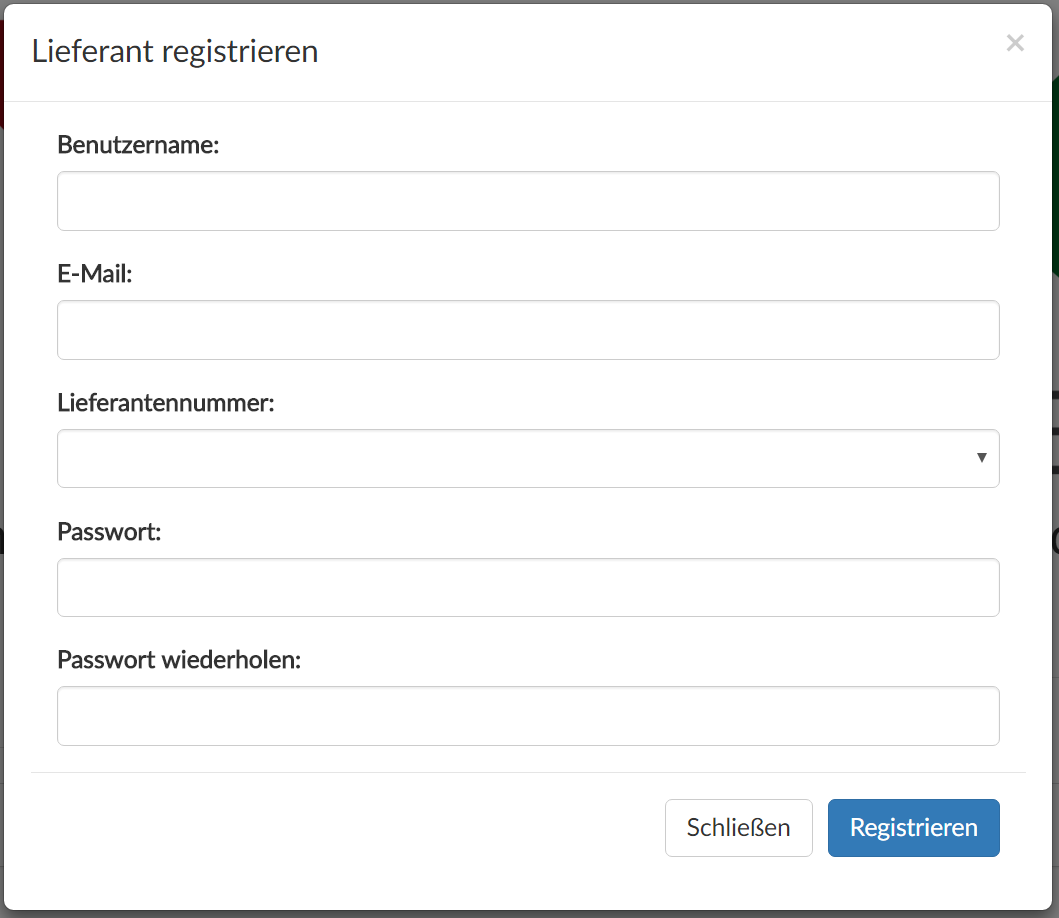
\includegraphics[width=17cm]{figures/registermock.png}
    \label{fig:takebill}
    \caption{Lieferant registrieren-Oberfläche}
\end{figure}

\newpage
In der unten stehenden Grafik ist das Ablaufdiagramm der Registrier-Funktion zu sehen.
\begin{figure}[!h]
    \centering
    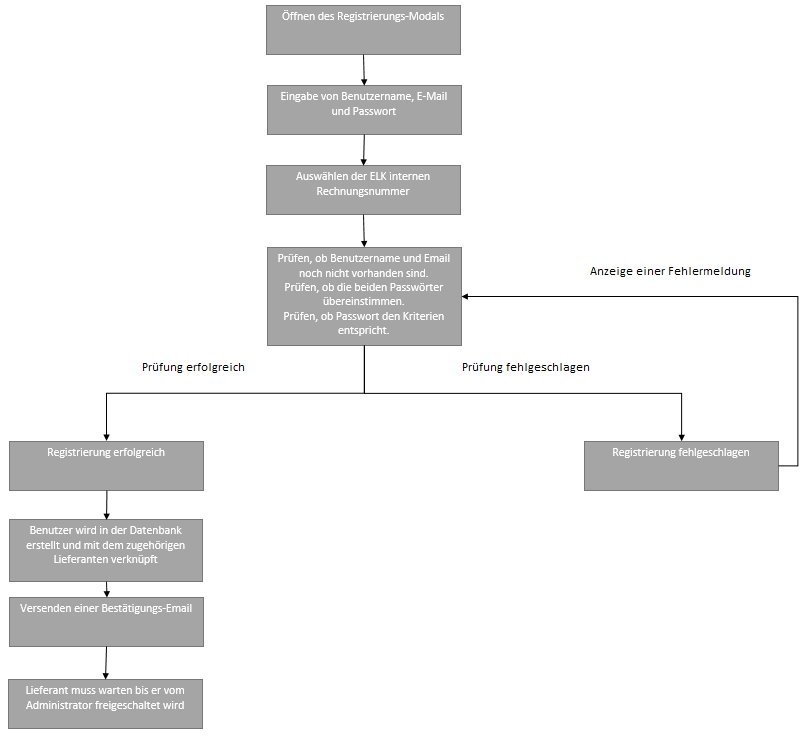
\includegraphics[width=17cm, height=18cm]{figures/register.png}
    \label{fig:register}
    \caption{Lieferant registrieren-Ablaufdiagramm}
\end{figure}
\newpage

\section{Login}
Die Plattform beinhaltet zwei unterschiedliche Login-Masken, wenn man die Startseite der elektronischen Rechnungsplattform betritt, zum einen den Lieferanten-Login und zum anderen den Buchhaltungs-/Administrator-Login. Wenn Benutzername und Passwort eingegeben wurden, wird auf deren Existenz und Gültigkeit mithilfe der Datenbank geprüft. Das Passwort wird zusätzlich verschlüsselt\footnote{\url{https://laravel.com/docs/5.2/hashing}} übertragen, um es mit dem aus der Datenbank vergleichen zu können. Danach wird untersucht, ob der Nutzer die jeweiligen Rechte für die Login-Maske besitzt, das bedeutet, dass der Lieferant den Lieferanten-Login benutzt. Beim Lieferant wird zusätzlich überprüft, ob seinem Benutzer ein Lieferant zugewiesen ist. Wenn eine der oben genannten Überprüfungen fehlschlägt, wird dem aktuellen Benutzer eine entsprechende Fehlermeldung angezeigt, die das aufgetretene Problem beschreibt. Falls der Login-Versuch erfolgreich durchgeführt wurde, wird eine Benutzer-Session erstellt und der Nutzer auf dessen jeweilige Seite weitergeleitet. (z.B.: Lieferant gelangt auf Lieferanten-Seite) Zudem wird überprüft, ob das Passwort des Benutzers geändert werden muss (z.B.: Passwortänderungsintervall wurde überschritten). Falls ja, wird der betreffende Nutzer direkt auf die Passwort ändern-Webseite weitergeleitet.

\newpage
Unten sehen Sie einen Ausschnitt aus der Login-Methode des Lieferanten. Es finden Überprüfungen statt, ob der Benutzer existiert, ob er gesperrt ist, ob er die Rechte eines Lieferanten besitzt. Dann wird das eingegebene Passwort verschlüsselt und mit dem Passwort aus der Datenbank verglichen. Wenn alle Prüfungen erfolgreich waren, wird eine Session erstellt und der Benutzer weitergeleitet. Wenn eine Prüfung fehlschlägt, wird dem Benutzer eine aussagekräftige Fehlermeldung angezeigt.

\lstset{language=PHP,caption={Login-Methode, für kompletten Ausschnitt siehe S. \pageref{logincode}},label=login}
\begin{lstlisting}
if (isset($user)) {
   if ($user->locked == 0) {
	   if ($user->rights == 'supplier') {
		  if (Hash::check($enteredpassword, $user->password)) {
			  Session::put('supplier', $user->id);
			  return redirect('supplier')->with('status', 'Sie haben sich erfolgreich als Lieferant angemeldet!');
		  } else {
			  return back()->with('status', 'Sie haben ein falsches Passwort eingegeben!')->withInput();
		  }
	  } else {
		  return back()->with('status', 'Sie besitzen nicht die benötigten Rechte um sich hier anzumelden!')->withInput();
	  }
  } else {
	  return back()->with('status', 'Der Benutzer wurde noch nicht freigeschaltet!')->withInput();
  }
}
\end{lstlisting}

\newpage
In den beiden Abbildungen sind die beiden Login-Masken für den Buchhalter und den Lieferanten zu sehen.
\begin{figure}[!h]
    \centering
    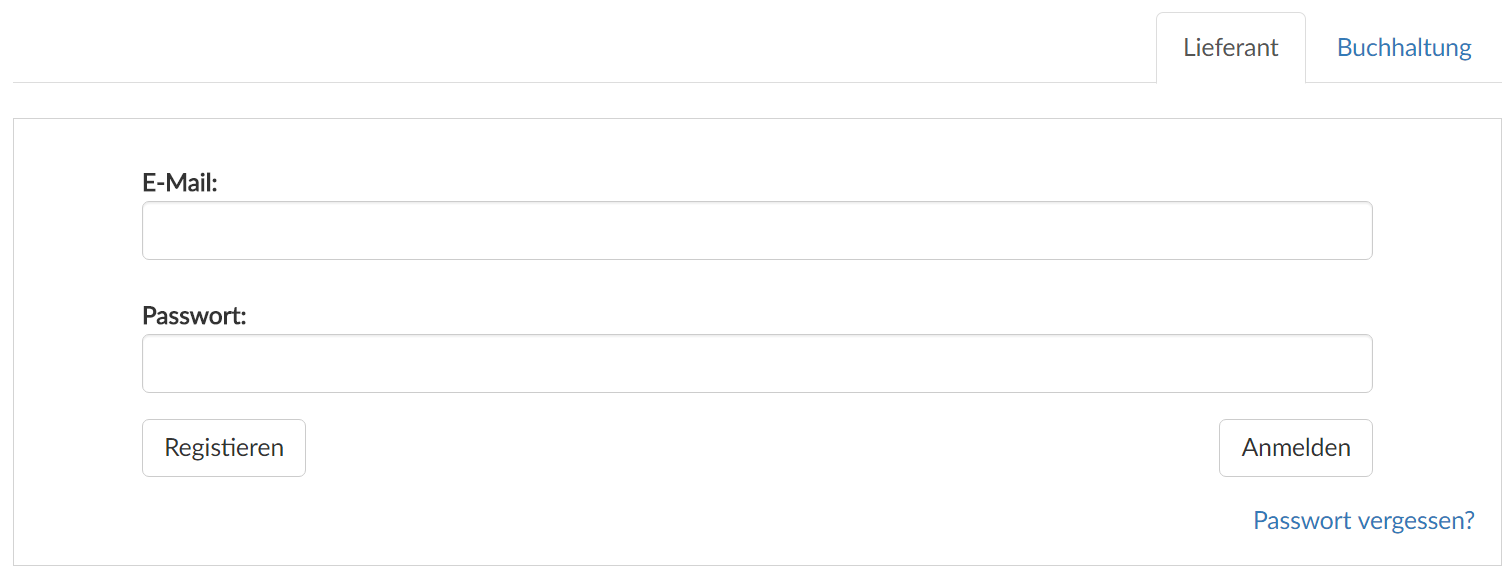
\includegraphics[width=17cm]{figures/loginmask.png}
    \label{fig:takebill}
    \caption{Login-Oberfläche Lieferant}
\end{figure}

\begin{figure}[!h]
    \centering
    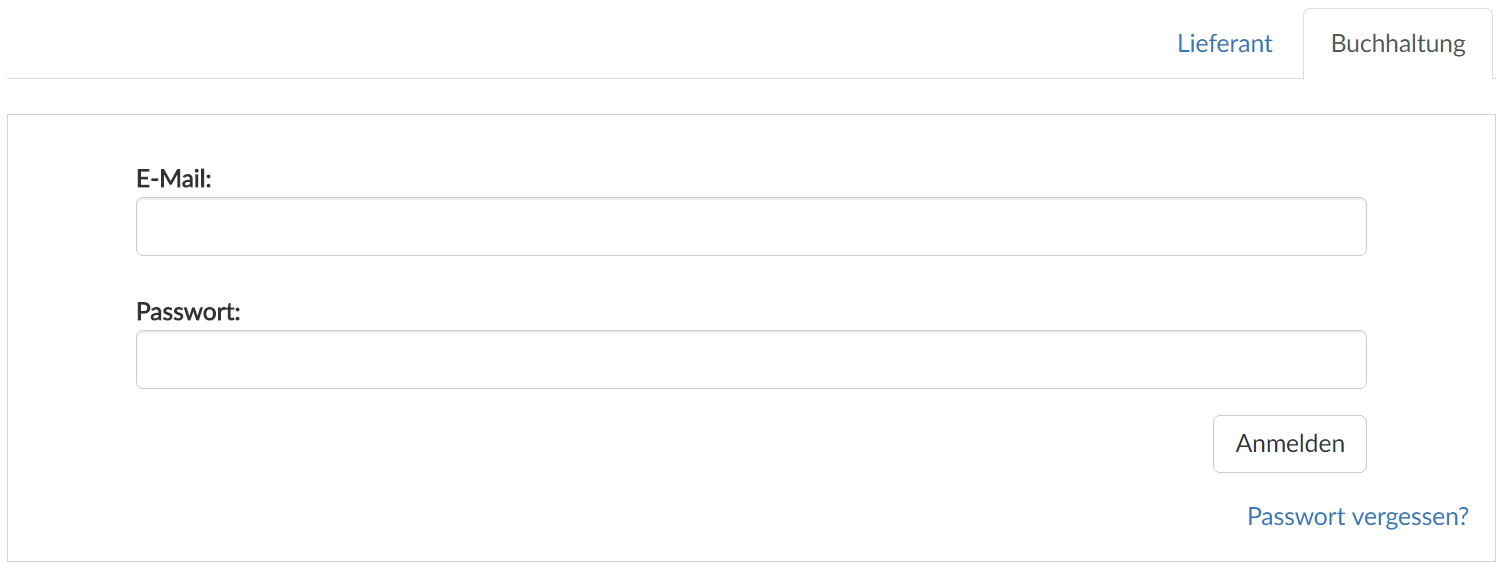
\includegraphics[width=17cm]{figures/loginbuchmock.png}
    \label{fig:takebill}
    \caption{Login-Oberfläche Buchhaltung}
\end{figure}


\newpage
In der unten stehenden Grafik ist das Ablaufdiagramm der Login-Funktion zu sehen.
\begin{figure}[!h]
    \centering
    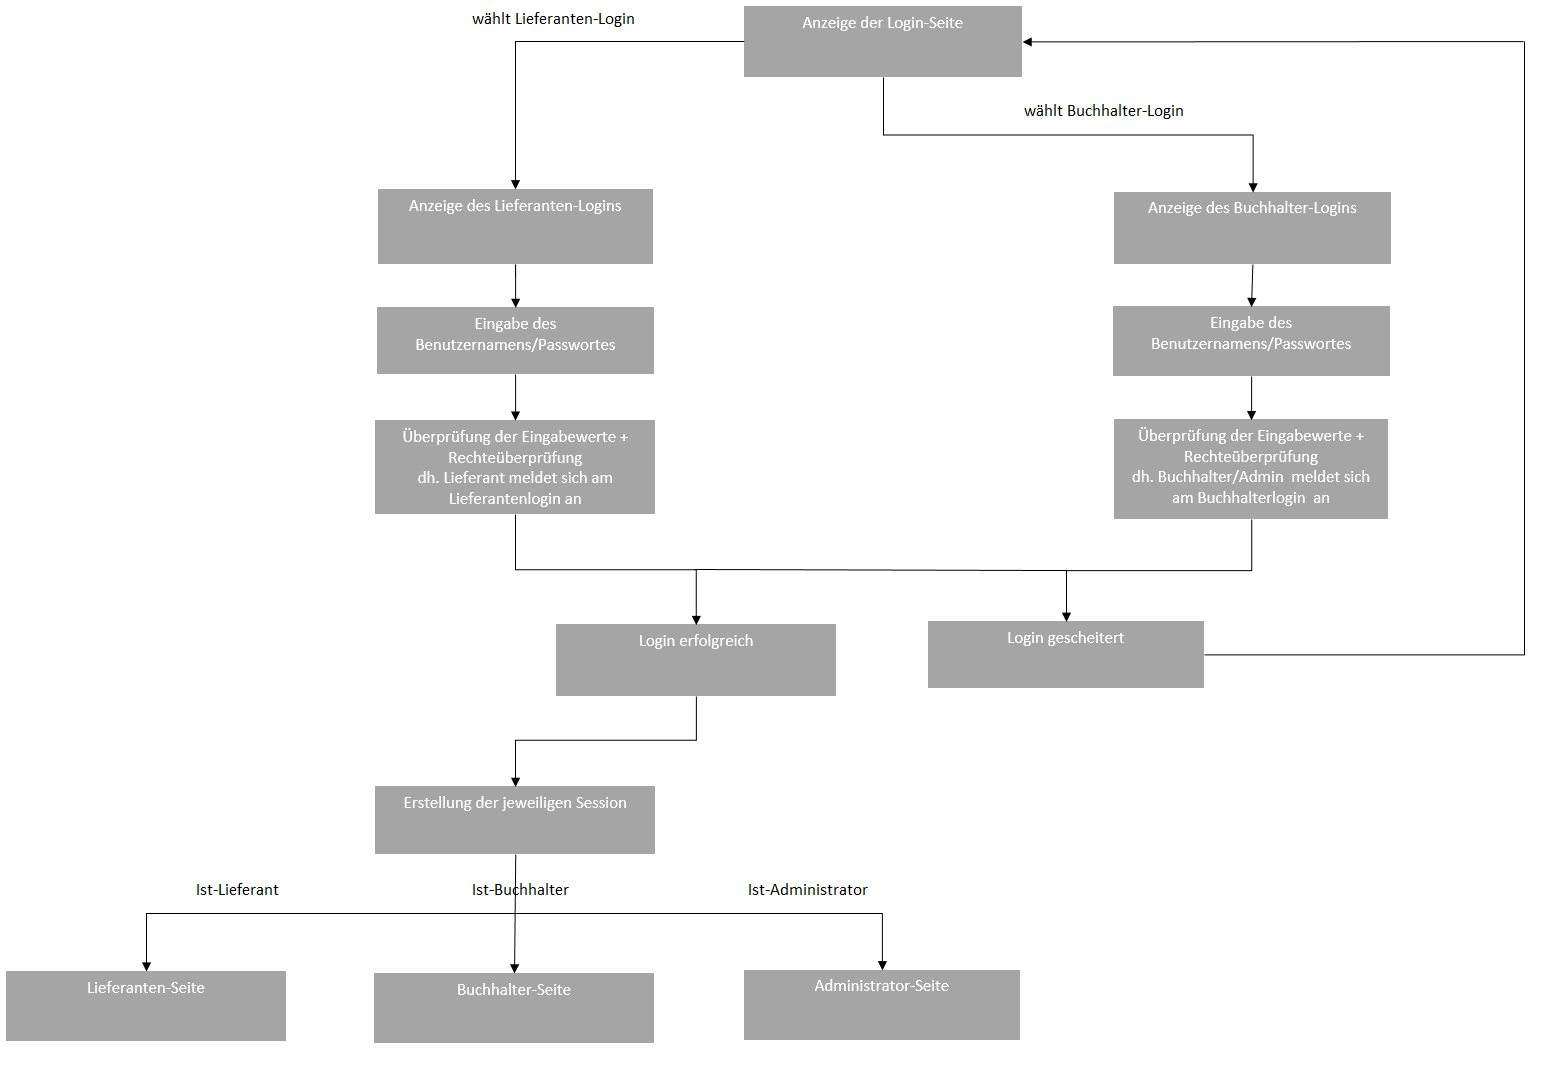
\includegraphics[width=17cm, height=15cm]{figures/login.jpg}
    \label{fig:login}
    \caption{Login-Ablaufdiagramm}
\end{figure}
\newpage

\section{Passwort vergessen}
Falls ein Benutzer (Lieferant, Buchhalter) sein Passwort vergisst, kann er dies ohne Probleme zurücksetzen. Dazu öffnet er die \glqq Passwort vergessen\grqq -Schaltfläche. Darin trägt er seine E-Mail-Adresse ein. Danach wird geprüft, ob die E-Mail-Adresse in der Datenbank existiert. Falls diese vorhanden ist, wird eine E-Mail mit einem Link zum Zurücksetzen an den jeweiligen Benutzer gesendet. Der Anwender öffnet danach seine E-Mails und gelangt auf eine Seite, auf der er sein Passwort verändern kann. Auch hier wird geprüft, ob die beiden Passwörter übereinstimmen und ob sie den Passwortkriterien der jeweiligen Benutzergruppe entsprechen. Wenn eine Überprüfung fehlschlägt, wird dem Benutzer eine entsprechende Fehlermeldung angezeigt. Falls alles erfolgreich durchgeführt wurde, wird der Anwender auf die Login-Seite weitergeleitet und er kann sich mit seinem neuen Passwort normal anmelden. 

Unten sehen Sie einen Ausschnitt aus der \glqq Passwort vergessen\grqq{} -Methode. Zuerst werden die Regeln festgelegt, denen die Eingabe entsprechen muss (Passwortkriterien, neues Passwort muss zweimal gleich eingegeben werden). Danach wird geprüft, ob die Angaben den Regeln entsprechen, wenn nicht, werden dem Benutzer die Fehler ausgegeben und falls sie stimmen wird der Benutzer zur Login-Seite weitergeleitet.

\lstset{language=PHP,caption={Passwort vergessen-Methode, für kompletten Ausschnitt siehe S. \pageref{vergessencode}},label=vergessen}
\begin{lstlisting}
$rules = array(
	'newpassword' => $criterias[0],
	'repeat_newpassword' => 'required|same:newpassword',
);

$validator = Validator::make(Input::all(), $rules, $messages);

if ($validator->fails()) {
	$messages = $validator->messages();
		return redirect()->back()->withErrors($validator);
} 
else {
	$password = $request->input('newpassword');
	User::find($id)->update(['password' => $password, 'has_changed' => 1]);
		return redirect('/');
}
\end{lstlisting}
\newpage
In den Abbildungen ist die E-Mail zu sehen, die der Benutzer erhält, wenn er sein Passwort zurücksetzen möchte, sowie die \glqq Passwort vergessen\grqq{} -Seite. 
\begin{figure}[!h]
    \centering
    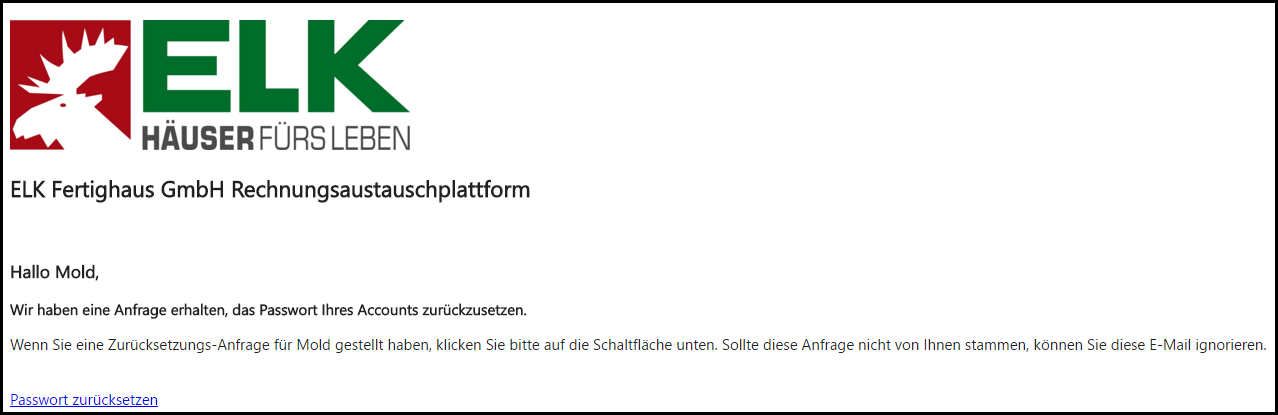
\includegraphics[width=17cm]{figures/mail.png}
    \label{fig:takebill}
    \caption{Passwort Vergessen E-Mail}
\end{figure}
\\ \\
\begin{figure}[!h]
    \centering
    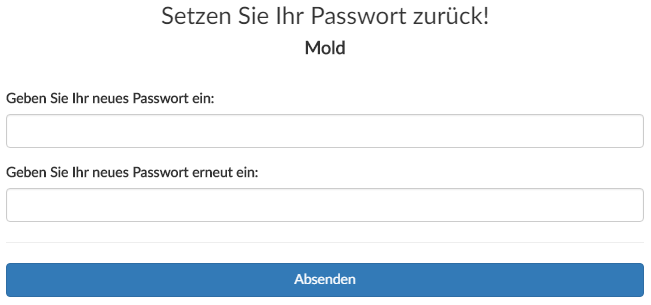
\includegraphics[width=17cm]{figures/vergessenmock.png}
    \label{fig:takebill}
    \caption{Passwort vergessen-Oberfläche}
\end{figure}

\newpage
In der unten stehenden Grafik ist das Ablaufdiagramm der \glqq Passwort vergessen\grqq{} -Funktion zu sehen.
\begin{figure}[!h]
    \centering
    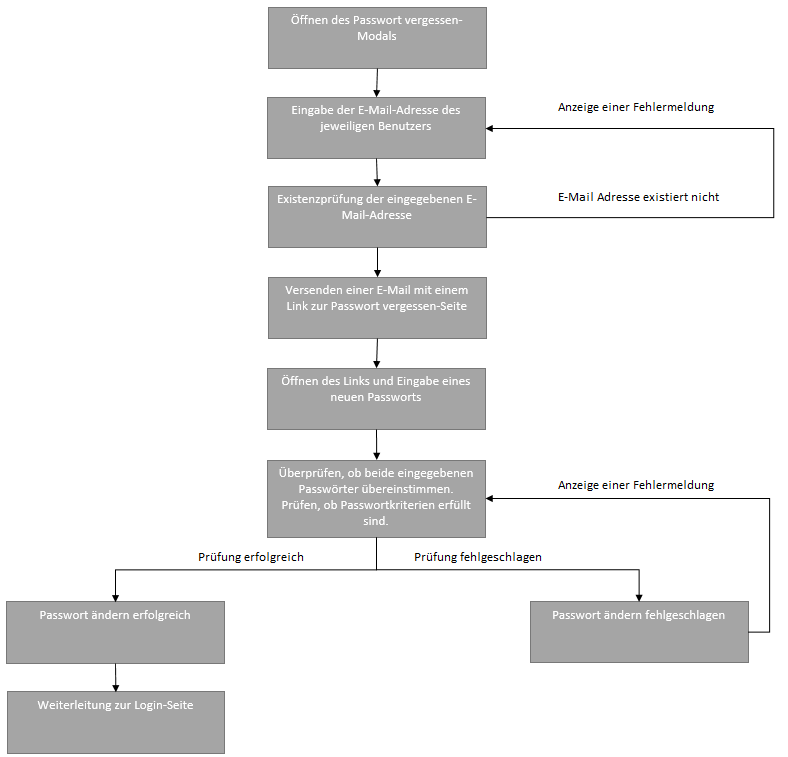
\includegraphics[width=17cm, height=15cm]{figures/vergessen.PNG}
    \label{fig:login}
    \caption{Passwort vergessen-Ablaufdiagramm}
\end{figure}
\newpage

\section{Rechnung hochladen}
Die \glqq Rechnung hochladen\grqq{}-Funktion steht nur einem Lieferanten zur Verfügung. Sie wird als zweites Tab angezeigt, neben den von ihm noch offenen Rechnungen. Zu Beginn füllt der Lieferant alle Felder des Formulars aus und wählt eine PDF, welche sich in seinem Dateiverzeichnis befinden muss, aus. Nach dem Klicken auf den Hochladen-Button werden die Größe der PDF-Datei und die eingetragenen Beträge überprüft. Erst wenn diese Felder die Kriterien erfüllen, wird die Rechnung in der Datenbank erstellt und die PDF-Datei in unserem Filesystem abgespeichert. Wenn der Vorgang erfolgreich durchgeführt wurde, wird ein weiterer Eintrag in die \glqq upload.log\grqq{} -Datei geschrieben und eine Erfolgsmeldung erscheint. Jedoch, wenn die Kriterien nicht erfüllt werden, wird eine Fehlermeldung angezeigt, die den Lieferanten bei der Fehlerausbesserung behilflich ist. \\

Ein Eintrag in der Log-Datei sieht wie folgt aus: \newline 
\textit{[2016-03-05] - [16:45:39] - [80536] - [46]}

\newpage
Hier folgt ein Code-Ausschnitt aus der \glqq Rechnung hochladen\grqq{}-Funktion. Am Beginn des Codes wird überprüft, ob alle Input-Felder ausgefüllt sind. Darauf folgt die Überprüfung, ob es sich bei der Datei um eine PDF-Datei handelt und nur dann wird der weitere Code ausgefüllt. Falls diese Kriterien erfüllt sind, wird die Rechnung in der Datenbank angelegt, die Datei hochgeladen und der PDF-Name zur Rechnung hinzugefügt. Das Loggen der Hochladen-Funktion und die Verweise auf die Seiten mit den anzuzeigenden Meldungen, die als Nächstes angezeigt werden, sind in dem Code-Fragment nicht vorhanden. Diese können im gesamten Code nachgeschlagen werden.



\lstset{language=PHP,caption={Rechnung hochladen-Funktion, für kompletten Ausschnitt siehe S. \pageref{hochladencode}},label=Rechnung-hochladen}
\begin{lstlisting}
// Die angelegten Rules nehmen und mit den Inputs prüfen
$validator = Validator::make(Input::all(), $rules, $messages);
// Wenn etwas fehlt oder fehlgeschlagen ist, dann komm ich zurück auf meine Seite mit den fehlenden Inputs
if ($validator->fails()) {
    return redirect('supplier#panel_uploadbill')->withInput()->withErrors($validator);
}

// Wenn Datei eine PDF ist
if ($pdf->getClientOriginalExtension() == 'pdf') {
    // Rechnung anlegen
    $bill = Bill::create(array(
        'amount' => $amount,
        'tax_amount' => $tax_amount,
        'document_date' => $document_date,
        'external_billnumber' => $external_billnumber,
        'billtype_id' => $billtype_id,
        'currency_id' => $currency_id,
        'company_id' => $company_id,
        'supplier_id' => $supplier_id,
        'status' => 'ready',
    ));

    // PDF-name bilden mit der ID der Rechnung
    $pdfName = $bill->id.'.'.$pdf->getClientOriginalExtension();
    // speichern der PDF
    $pdf->move('../storage/app/pdfs/', $pdfName);

    // PDF zur Rechnung hinzuspeichern
    $bill->pdf_name = $pdfName;
    $bill->save();
}
\end{lstlisting}

\newpage
In dem unten zu sehenden Formular kann ein Lieferant eine Rechnung hochladen. Dabei müssen alle Felder ausgefüllt sein.
\begin{figure}[!h]
    \centering
    \includegraphics[width=17cm]{figures/upload.png}
    \label{fig:takebill}
    \caption{Rechnung hochladen-Oberfläche}
\end{figure}

\newpage
Das nachfolgende Bild zeigt den Ablauf der \glqq Rechnung hochladen\grqq{}-Funktion.
\begin{figure}[!h]
    \centering
    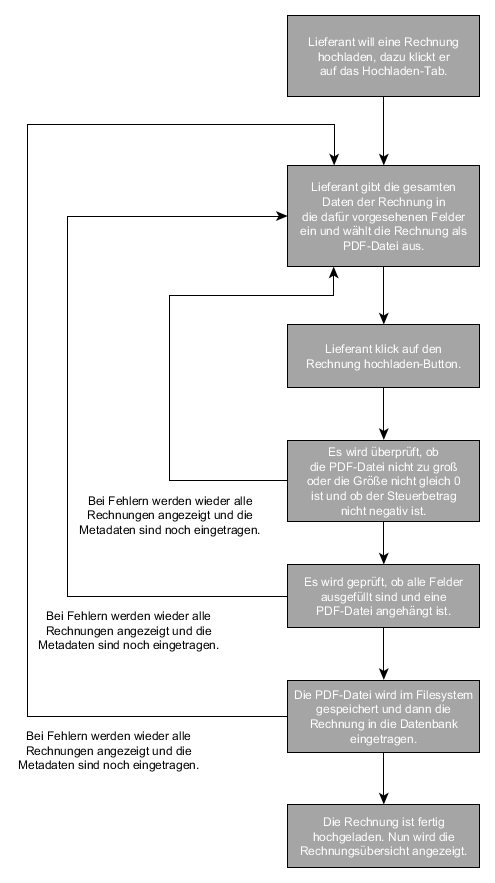
\includegraphics[width=12cm]{figures/rechnunghochladen.png}
    \label{fig:takebill}
    \caption{Rechnung hochladen-Ablaufdiagramm}
\end{figure}

\newpage

\section{Rechnung holen}
Die bereits hochgeladenen Rechnungen werden der Buchhaltung in absteigender Reihenfolge angezeigt. Wenn der Buchhalter den \glqq Rechnung holen\grqq{} -Button in der Rechnungstabelle klickt, wird zuerst eine XML-Datei aus den Metadaten der Rechnung mit den Informationen aus der Datenbank erstellt. Da die Plattform von mehreren Buchhaltern genutzt wird, wird überprüft ob die Rechnung, die geholt werden soll, bereits verarbeitet wurde. Danach wird eine E-Mail erstellt, die die XML-Datei sowie die Rechnung als PDF, die vom Lieferanten hochgeladen wurde, als Anhang besitzt. Die E-Mail wird in eine sogenannte Warteschlange geschoben und wird später versendet. Dies dient dazu, dass der aktuelle Benutzer nicht warten muss, bis die E-Mail an die rechnerunterstützte Buchhaltung versendet wurde, sondern gleich mit seiner Arbeit fortfahren kann. Alle zehn Sekunden wird eine E-Mail aus der Warteschlange entfernt und versendet. Eine Minute nachdem diejenige E-Mail mit den Anhängen versendet wurde, wird die Rechnungs PDF-Datei und die XML-Datei in ein Archiv-Verzeichnis verschoben. Außerdem wird in der Datenbank der Status \glqq geholt\grqq{} zugewiesen, daher wird diese auch nicht mehr in der Rechnungstabelle angezeigt. Des Weiteren wird ein Eintrag in der taken.log Datei erstellt. Dieser Eintrag beinhaltet das aktuelle Datum, die genaue Uhrzeit sowie die Rechnungsnummer und Lieferantennummer. Die weitere Verarbeitung der Eingangsrechnung übernimmt die computerunterstützte Buchhaltung der Firma ELK Fertighaus GmbH.
\newpage
Unten sehen Sie einen Ausschnitt aus der \glqq Rechnung holen\grqq{} -Methode. Die Methode erstellt die E-Mail und verschiebt sie in die Warteschlange. Außerdem wird der Job erstellt, der die XML-Datei und die Rechnungsdatei in ein Archiv-Verzeichnis verschiebt.

\lstset{language=PHP,caption={Rechnung holen, für kompletten Ausschnitt siehe S. \pageref{holencode}},label=holen}
\begin{lstlisting}
//Mail erstellen und Anhänge anhängen
Mail::later(10, 'mail.bill', ['billinfo' => $bill], function ($m) use ($bill, $filecontents) {
	$m->from(env('MAIL_SENDER', ''), env('MAIL_NAME', 'ELK_Rechnungsplattform'));
	$m->to($bill->email, $bill->username)->subject('Rechnungsnummer: '.$bill->id);
	$m->attach('public/pdfs/'.$bill->pdf_name);
	$m->attach('storage/app/'.$filecontents[0]);
});

//Dateien verschieben
$delete = (new SendBillEmail($bill, $filecontents))->delay(60);
$this->dispatch($delete); 
\end{lstlisting}

\vspace{1cm}
Ein Eintrag in der Log-Datei sieht wie folgt aus: \newline 
\textit{[2016-02-27] - [17:10:26] - [80536] - [5]}

\vspace{1cm}
In der Abbildung unten ist die Oberfläche zu sehen, wo der Buchhalter die Rechnung holen kann.
\begin{figure}[!h]
    \centering
    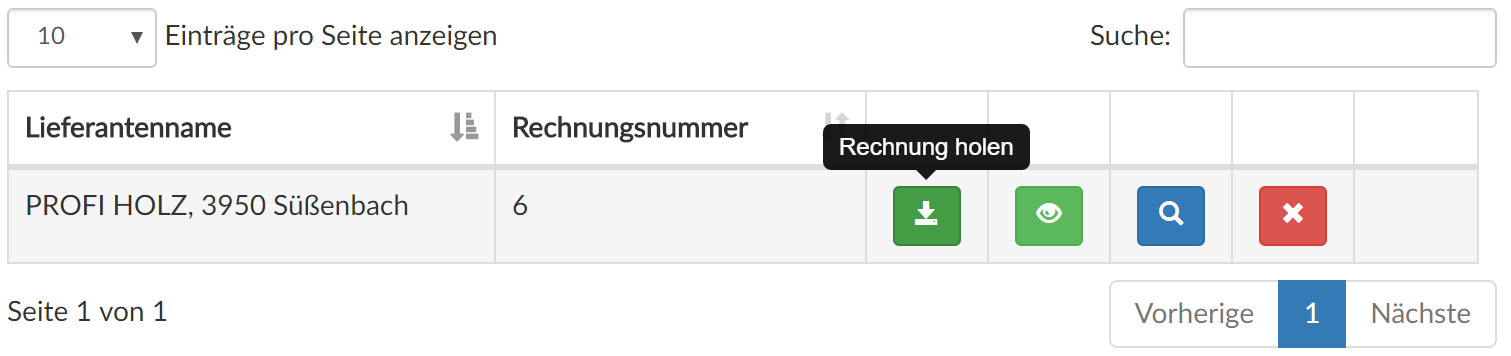
\includegraphics[width=15cm]{figures/holencode.png}
    \label{fig:takebill}
    \caption{Rechnung holen-Oberfläche}
\end{figure}

\newpage
Der folgende Ausschnitt zeigt und beschreibt den Aufbau der XML-Datei, die der Buchhaltung zugesendet wird. Weiters ist eine Beschreibung der einzelnen Elemente gegeben.
\lstset{
  language=XML,
  morekeywords={encoding,
    INVOIC02, IDOC, E1EDKA1, E1EDK03, E1EDK01, E1EDS01},
    caption={Generierte XML-Datei},label=billxml
}
\begin{lstlisting}
<?xml version="1.0" encoding="UTF-8" standalone="no"?>
<INVOIC02>
  <IDOC BEGIN="1">
    <E1EDKA1 SEGMENT="1">
      	<PARVW>RE</PARVW>	-> Rechnungsempfänger
      	<LIFNR>001</LIFNR> 	-> Standort (001 = ELK Österreich)
    </E1EDKA1>
    <E1EDKA1 SEGMENT="1">
      	<PARVW>BK</PARVW>	-> Rechnungssteller
      	<LIFNR>80536</LIFNR>	-> ELK Lieferantennummer
    </E1EDKA1>
    <E1EDK03 SEGMENT="1">
      	<IDDAT>012</IDDAT>	-> Datumsformat
      	<DATUM>20160305</DATUM>	-> Datum der Rechnung
    </E1EDK03>
    <E1EDK01 SEGMENT="1">
      	<CURCY>EUR</CURCY>	-> Währung
      	<BELNR>888</BELNR>	-> Belegnummer
      	<BSART>G</BSART>	-> Art der Rechnung z.B.: Gutschrift
    </E1EDK01>
    <E1EDS01 SEGMENT="1">
      	<SUMID>011</SUMID>	-> Art des Betrags z.B.: Steuerbetrag
      	<SUMME>88</SUMME>	-> Summe des Steuerbetrags
    </E1EDS01>
    <E1EDS01 SEGMENT="1">
      	<SUMID>005</SUMID>	-> Art des Betrags z.B.: Rechnungsbetrag
      	<SUMME>88</SUMME>	-> Summe des Rechnungsbetrags
    </E1EDS01>
  </IDOC>
</INVOIC02>
\end{lstlisting}
\newpage
In der unten stehenden Grafik ist das Ablaufdiagramm der \glqq Rechnung holen\grqq{} -Funktion zu sehen.
\begin{figure}[!h]
    \centering
    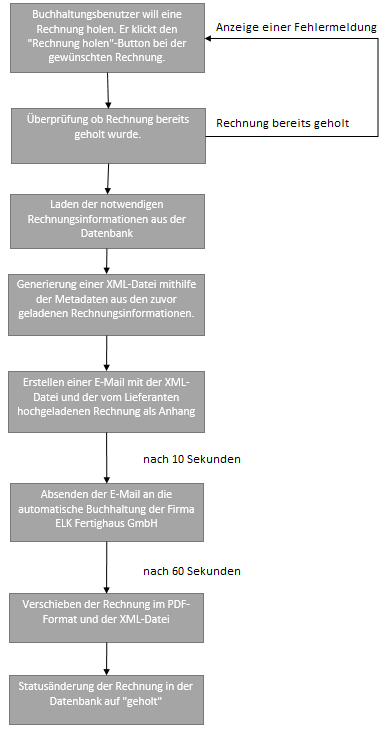
\includegraphics[width=10cm]{figures/billtaken.png}
    \label{fig:takebill}
    \caption{Rechnung holen-Ablaufdiagramm}
\end{figure}
\newpage

\section{Datenbank-Synchronisation}
Die Datenbank-Synchronisation wird automatisch durch einen Cronjob aufgerufen.

Den Cronjob selbst führt das System jede Minute aus, doch die Datenbank synchronisiert sich nur um Mitternacht. Laravel stellt ein Feature zur Verfügung, das durch einen Cronjob aufgerufen wird. In diesem Feature gibt man an, zu welcher Uhrzeit eine ausprogrammierte Funktion (z.B.: Datenbank-Synchronisation) aufgerufen werden soll.

Durch die Datenbank-Synchronisation werden die Lieferanten-Daten der Rechnungsplattform-Datenbank mit er Datenbank der Firma ELK abgeglichen und gleichgestellt. Die Excel-Datei, in der die Lieferanten-Daten der Firma ELK gespeichert sind, muss von den Datenbankexperten des Unternehmens jeden Tag erneuert werden, um eine Gleichheit der Datenbanken zu gewährleisten. Falls während der Synchronisation ein Fehler auftritt, wird der Vorgang abgebrochen und die Datenbank auf den zuvor herrschenden Stand zurückgesetzt.

Zu Beginn der Durchführung werden alle Lieferanten-Daten der Datenbank in eine Variable gespeichert und danach gelöscht. Die Benutzer, welche über Lieferanten-Rechte verfügen, werden von der Plattform gesperrt und die Excel-Datei wird eingelesen. Danach durchläuft die Funktion jeden einzelnen Eintrag der Excel-Datei und fügt diesen in die Datenbank ein. Falls einer der Lieferanten bereits einen Benutzer zugewiesen hat, wird dieser ebenfalls eingetragen und der Gesperrt-Status auf den, der vorher eingetragen war, geändert.

\newpage
Hier folgt ein Ausschnitt aus dem Code. Vor diesem Teil werden alle Lieferanten in eine Variable gespeichert und gelöscht. Außerdem speichert man die Benutzer ebenfalls ab und sperrt diese. Im Codestück wird die Excel-Datei mit den Lieferanten-Daten ausgelesen und verarbeitet. Danach legt die Funktion die einzelnen Lieferanten an und weist einen Benutzer zu, falls einer für diesen Lieferanten vorhanden ist. Nach dem Ausschnitt werden noch alle nicht gebrauchten Lieferanten-Benutzer aus der Datenbank gelöscht.
\lstset{language=PHP,caption={Datenbank-Synchronisation, für kompletten Ausschnitt siehe S. \pageref{datenbanksynchronisationcode}},label=Datenbank-Synchronisation}
\begin{lstlisting}
$file = storage_path('app').'\xlsxs\lieferanten.xlsx'; //Dateiname angeben
// Excel-Datei mithilfe des Plugins "Excel-Laravel" auslesen
$results = Excel::selectSheetsByIndex(0)->load($file, 'UTF-8')->get(array('adr_nr', 'adr_name', 'adr_uid'));
// Alle Einträge der Datei durchlaufen
foreach ($results as $row) {
    $supplier = new Supplier();
    $supplier->id = $row->adr_nr;
    $supplier->adr_name = $row->adr_name;
    $supplier->adr_uid = $row->adr_uid;

    if ($oldSup->contains('id', $row->adr_nr) == true) {
        // die alten Lieferanten durchgehen
        foreach ($oldSup as $item) {
            // schauen, wo die ADR_NR der alten Lieferanten gleich dem neuen ADR_NR ist
            if ($item->id == $row->adr_nr) {
                $supplier->user_id = $item->user_id;
                $supplier->newRegistered = $item->newregistered;

                // alle LieferantenUser durchgehen
                foreach($oldUser as $item2){
                    // Wenn die ID vom Benutzer gleich der ist, zu welchen er gehört
                    if($item2->id == $item->user_id){
                        // Benutzer sperren oder freischalten
                        User::where('id', $item->user_id)->update(['locked' => $item2->locked]);
                    }
                }
            }
        }
    }
    $supplier->save();
}
\end{lstlisting}
\newpage
Unten ist noch die Fehlerbehandlung ersichtlich. Diese wird ausgeführt, falls ein Fehler während des Auslesevorgangs, der Erstellung der Lieferanten oder der Bearbeitung der Benutzer auftritt. Im Allgemeinen dient dieser Code dazu, dass die Datenbank wieder den vorher herrschenden Stand zurückerlangt.
\lstset{language=PHP,caption={Datenbank-Synchronisation Fehlerbehandlung, für kompletten Ausschnitt siehe S. \pageref{datenbanksynchronisationfehlerbehandlungcode}},label=Datenbank-Synchronisation Fehlerbehandlung}
\begin{lstlisting}
// Falls etwas fehlschlägt
User::where('rights', 'supplier')->delete();
foreach($oldUser as $item){
    User::where('id', $item->id)->update(['locked' => $item->locked]);
}
Supplier::whereNotNull('id')->delete();
foreach($oldSup as $item){
    $item->save();
}
$this->error('Die Datenbank wurde nicht synchronisiert, da ein Fehler aufgetreten ist.');
\end{lstlisting}

\newpage
Hier ist das Ablaufdiagramm der oben beschriebenen Datenbanksynchronisation angeführt.
\begin{figure}[!h]
    \centering
    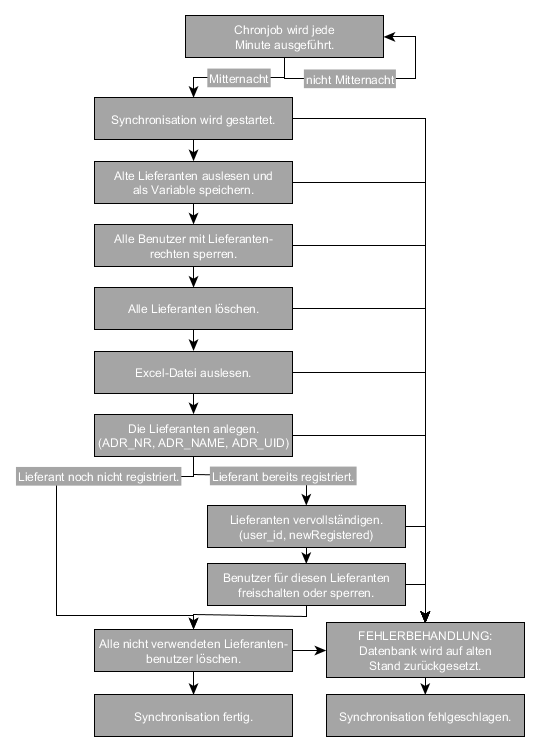
\includegraphics[width=15cm]{figures/DatenbankSynchronisieren.png}
    \label{fig:datenbanksynchronisation}
    \caption{Datenbanksynchronisation-Ablaufdiagramm}
\end{figure}
\newpage

\section{Backend-Administratoransicht}
Das Backend dient dazu, die gesamte Plattform zu verwalten. Man kann es auch als Administrator-Bereich ansehen, da das Backend nur für eine Person bestimmt ist. Der Benutzer, welcher in diesen Bereich gelangt, ist in der Datenbank bereits vorhanden und wird so mit ausgeliefert. Diese Ansicht kann erreicht werden, indem sich der Mitarbeiter mit den Anmeldedaten des Administrators am Buchhalter-Login anmeldet. Durch diese Anmeldung wird er sofort zur Administration umgeleitet.

Der Bereich beinhaltet folgende Komponenten:
\subsection{Startseite}
Wenn der Benutzer in den Administrator-Bereich gelangt, wird eine Startseite angezeigt. Auf dieser Seite werden die vier wichtigsten Daten der Plattform angezeigt. Bei den wichtigsten Daten handelt es sich um die Anzahl der registrierten Lieferanten, die Anzahl der freigeschalteten Lieferanten, die Anzahl der neuen Lieferanten und die Anzahl der offenen Rechnungen.
\begin{figure}[!h]
    \centering
    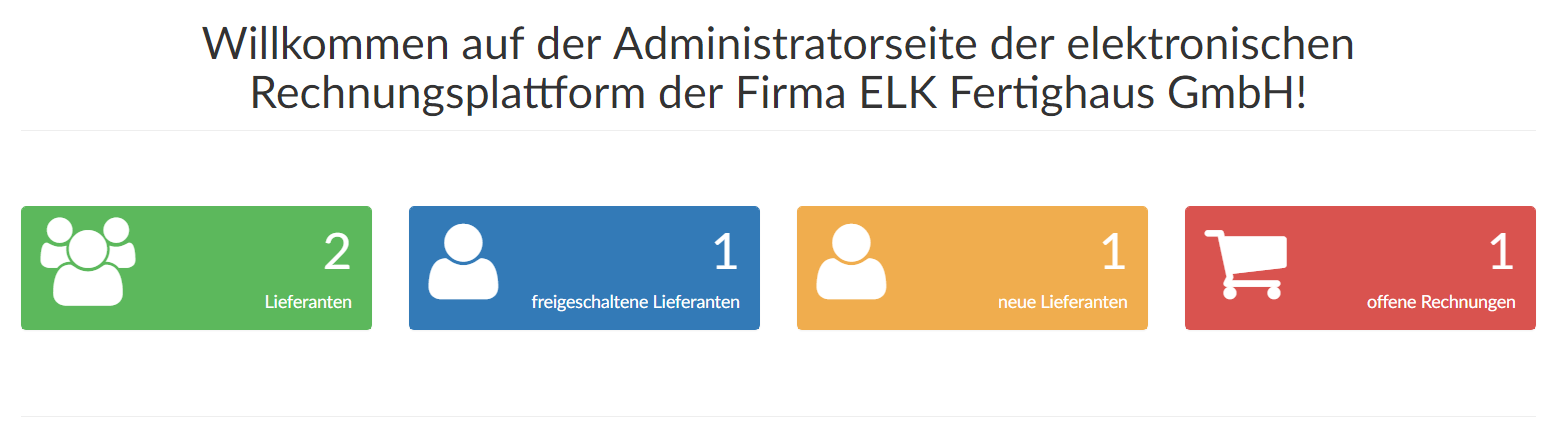
\includegraphics[width=15cm]{figures/backend.png}
    \label{fig:backendstartseite}
    \caption{Backend-Startseite}
\end{figure}
\newpage
\subsection{Lieferanten-Verwaltung}
In der Lieferanten-Verwaltung werden alle neu registrierten, registrierten und freigeschalteten Lieferanten angezeigt. Der Administrator besitzt die Rechte, dass er Lieferanten freischaltet, sperrt oder ganz löscht. Wenn der Administrations-Benutzer eine der Funktionen ausführt, wird der dazugehörige Lieferant über diese Durchführung informiert. Die Information erfolgt über eine E-Mail.
\begin{figure}[!h]
    \centering
    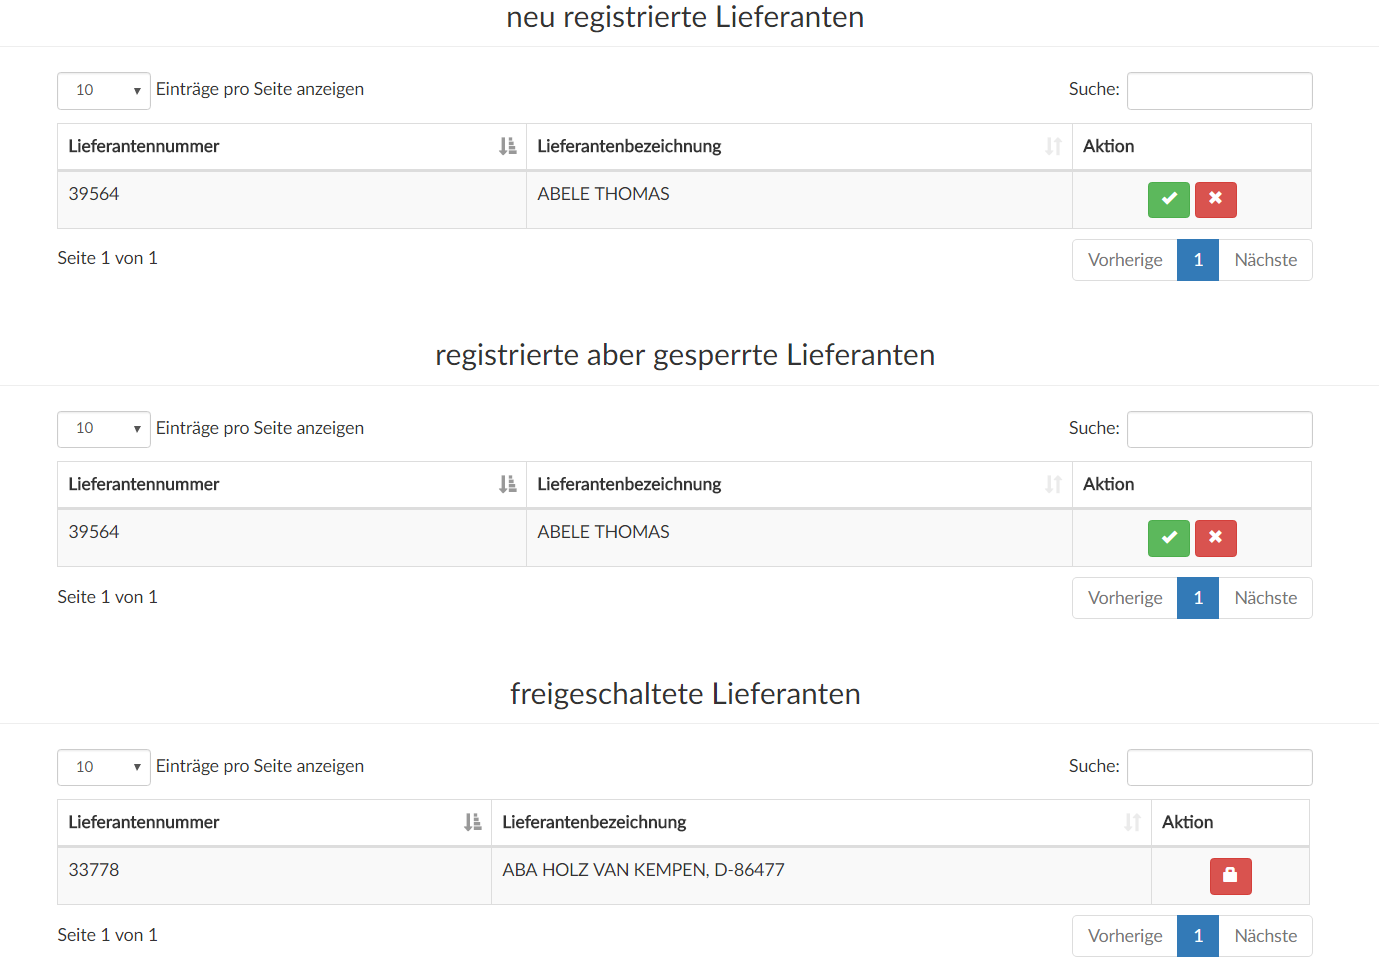
\includegraphics[width=17cm]{figures/lieferant.png}
    \label{fig:lieferantenverwaltung}
    \caption{Lieferanten-Verwaltung}
\end{figure}
\newpage
\subsection{Buchhaltungs-Verwaltung}
Die Buchhaltungs-Verwaltung dient dazu, mehrere Buchhalter für die Rechnungsplattform zu erstellen. (Im Gegensatz zur ursprünglichen Zielsetzung eines gemeinsamen Buchhalter-Nutzers.) Die einzelnen Buchhalter benötigen einen Benutzernamen und eine E-Mail. Über die angegebene E-Mail werden sie über das Erstellen benachrichtigt. Ebenfalls ist es dem Administrator möglich, die Buchhalter zu verwalten, das bedeutet, dass er die erstellten Benutzer freischalten, sperren und auch wieder löschen kann. Bei einem solchen Ereignis wird wieder eine Benachrichtigungs-E-Mail versendet.
\begin{figure}[!h]
    \centering
    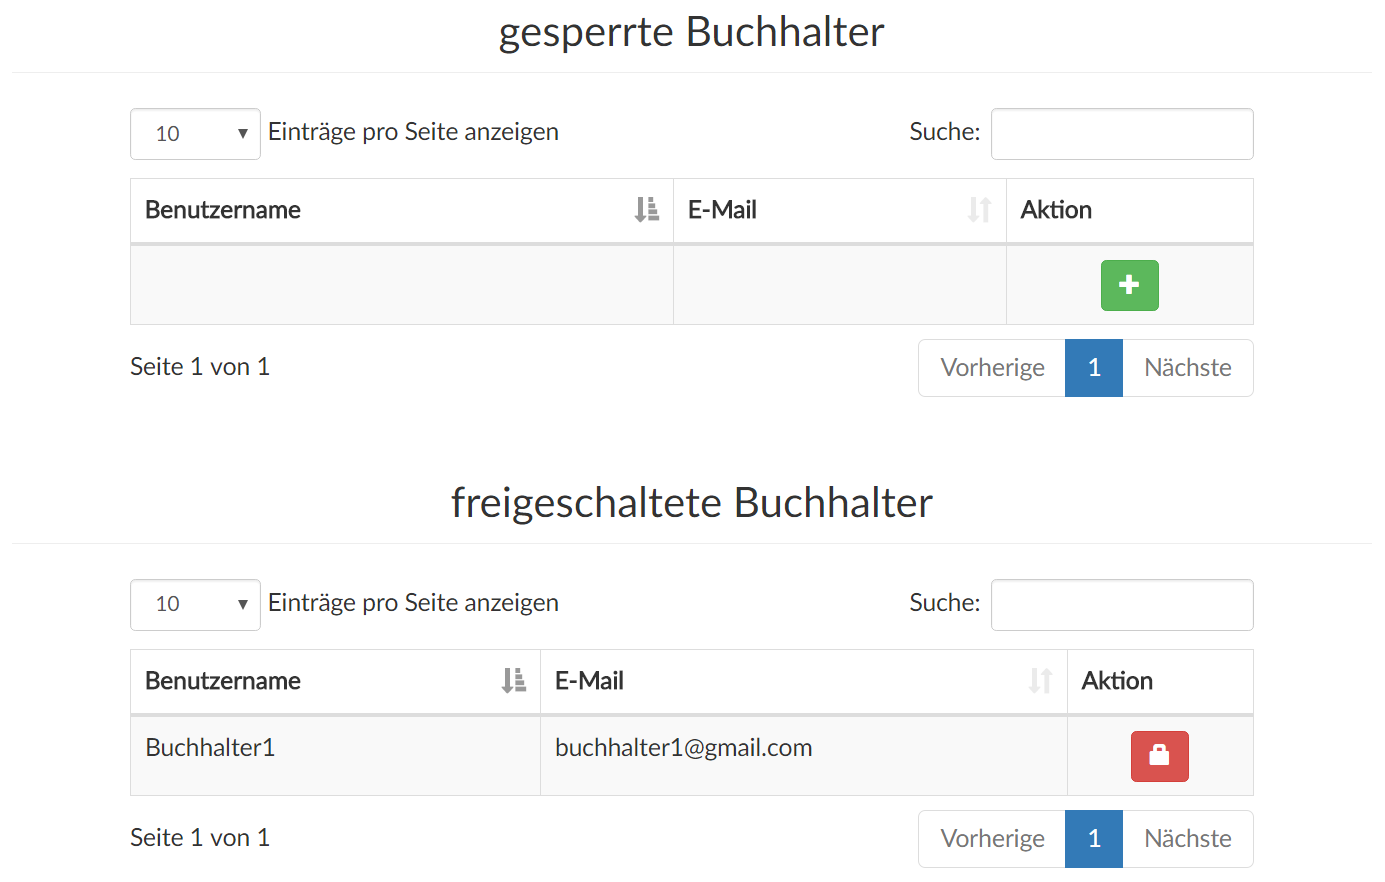
\includegraphics[width=17cm]{figures/buchhalter.png}
    \label{fig:buchhaltungsverwaltung}
    \caption{Buchhaltungs-Verwaltung}
\end{figure}
\newpage
\subsection{Passwort-Verwaltung}
Bei der Passwort-Verwaltung ist dem Administrator freigestellt, welche der vordefinierten Kriterien die Passwörter erfüllen müssen. Es ist auch möglich, die Vorgaben für die Buchhaltung, die Lieferanten und den Administrator getrennt zu definieren, wodurch eine unterschiedliche Sicherheitsstufe der Passwörter erreicht werden kann. Außerdem kann das Intervall, in welchem die Passwörter geändert werden müssen, festgelegt werden. Der Wert für die regelmäßige Änderung erstreckt sich von einer Woche bis zu höchstens fünf Wochen.
\begin{figure}[!h]
    \centering
    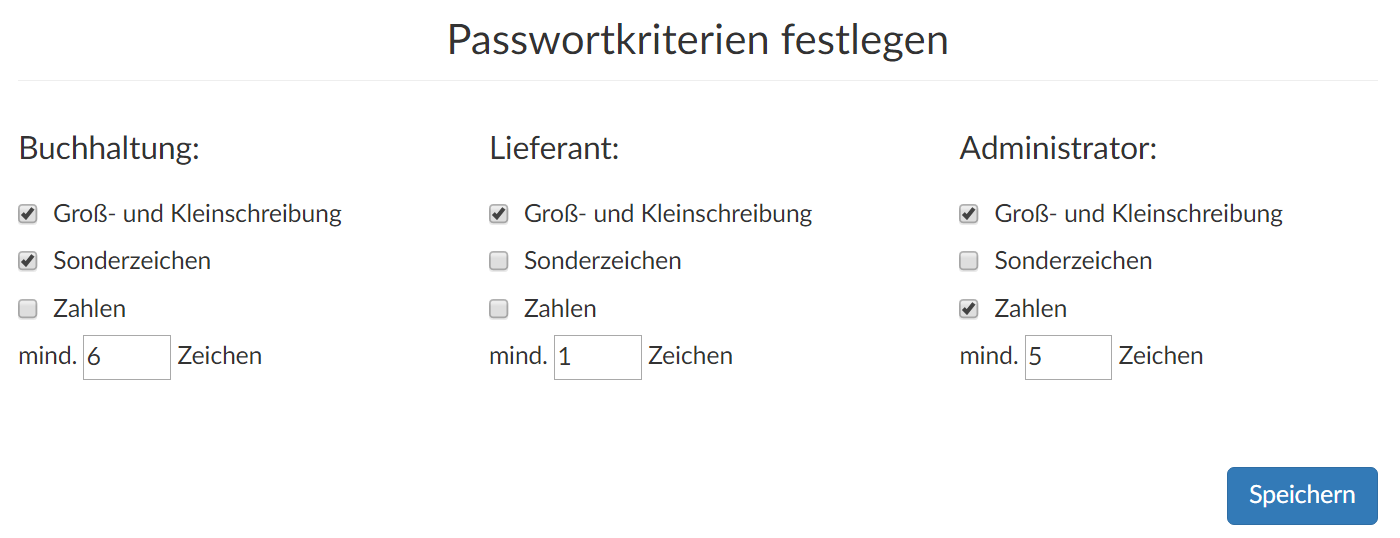
\includegraphics[width=15cm]{figures/kriterien.png}
    \label{fig:passwortkriterien}
    \caption{Passwortkriterien}
\end{figure}
\begin{figure}[!h]
    \centering
    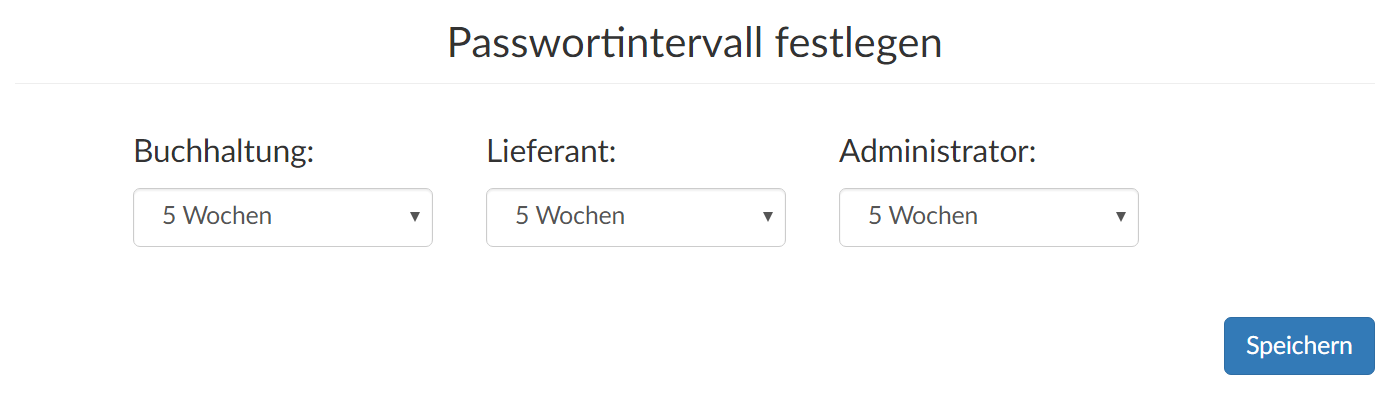
\includegraphics[width=15cm]{figures/intervall.png}
    \label{fig:passwortintervall}
    \caption{Passwort-Änderungsintervall}
\end{figure}
\newpage
\subsection{Standorte-Verwaltung}
Mit der Standorte-Verwaltung können neue Standorte der Firma hinzugefügt oder die bestehenden bearbeitet werden. Nach dem Erstellen eines Standortes ist es nicht möglich die Standort-Nummer zu verändern, sondern nur die Firmenbezeichnung. Löschen kann man keine Firma, denn sonst würden vielleicht Rechnungsdaten fehlen.
\begin{figure}[!h]
    \centering
    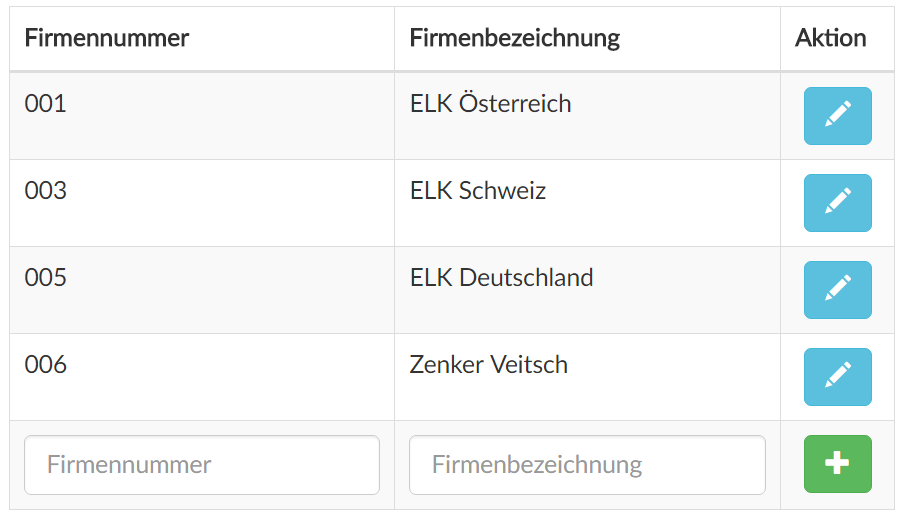
\includegraphics[width=15cm]{figures/standorte.png}
    \label{fig:standorteverwaltung}
    \caption{Standorte-Verwaltung}
\end{figure}
\newpage
\subsection{Währungs-Verwaltung}
Hier verwaltet der Administrator die Währungen, die eine Rechnung, Gutschrift und so weiter, aufweisen darf. Die verschiedenen Währungen können nur erstellt und bearbeitet werden.
\begin{figure}[!h]
    \centering
    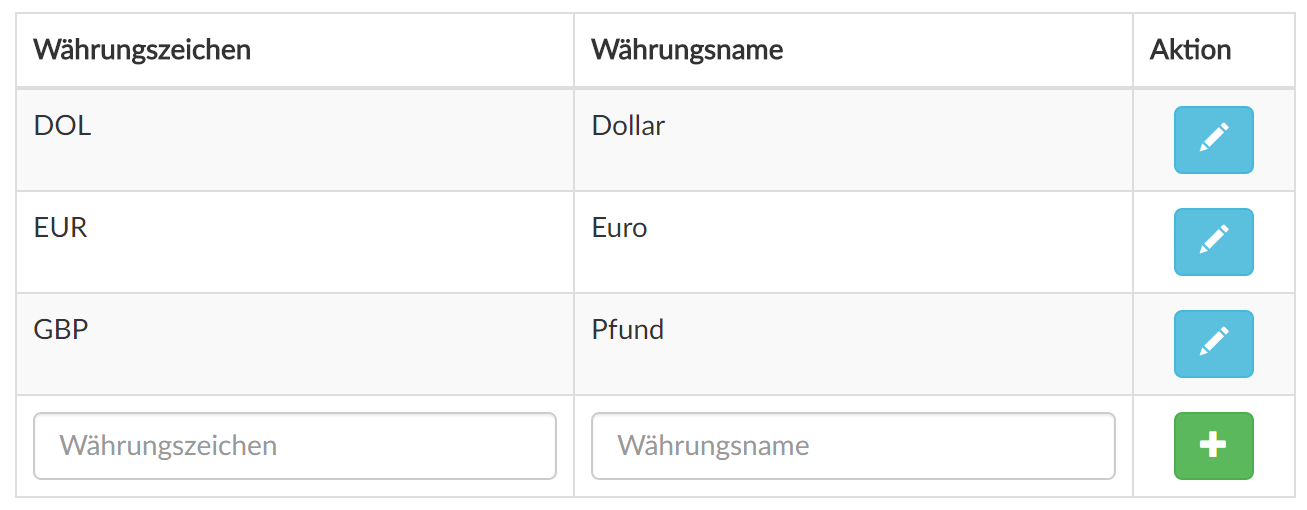
\includegraphics[width=15cm]{figures/waehrungen.png}
    \label{fig:waehrungsverwaltung}
    \caption{Währungs-Verwaltung}
\end{figure}

\subsection{Rechnungsarten-Verwaltung}
Auf dieser Ansicht können die Rechnungsarten erstellt und bearbeitet werden. Jede Art, die in dieser Übersicht angezeigt wird, kann beim Erstellen einer Rechnung vom Lieferanten ausgewählt werden. Die Löschen-Funktion ist nicht vorhanden, da beim Löschen Daten bei den bereits hochgeladenen Rechnungen fehlen könnten.
\begin{figure}[!h]
    \centering
    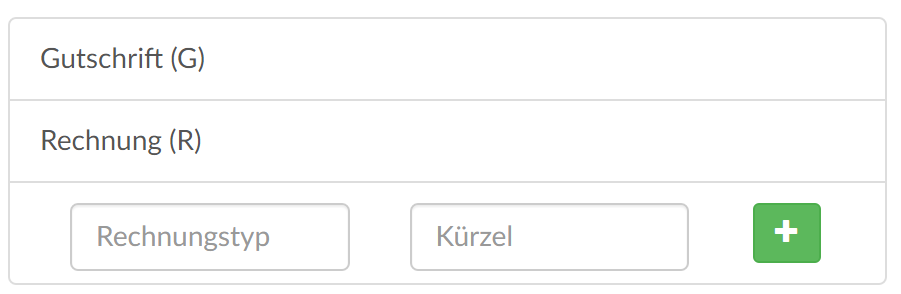
\includegraphics[width=15cm]{figures/rechnungsarten.png}
    \label{fig:rechnungsartenverwaltung}
    \caption{Rechnungsarten-Verwaltung}
\end{figure}
\newpage
\subsection{E-Mail-Verwaltung}
Mit der E-Mail-Verwaltung ist es dem Administrator möglich, die Benachrichtigungs-E-Mails zu verändern. An dieser Oberfläche gibt es drei Adressen zu verwalten. Die erste ist die wichtigste der gesamten Plattform, nämlich die des automatisierten Rechnungssystems. Auf diese E-Mail werden alle geholten Rechnungen gesendet. Die zweite wird benötigt, um die Buchhaltung über fehlerhafte Rechnungen zu informieren. Jedoch ist die Benachrichtigung auch in der Buchhalter-Oberfläche bei der Rechnungsübersicht erkennbar. Bei der dritten E-Mail handelt es sich um die, auf welche der Administrator zugreift. Auf diese E-Mail wird eine Benachrichtigung gesendet, wenn sich ein neuer Lieferant registriert.
\begin{figure}[!h]
    \centering
    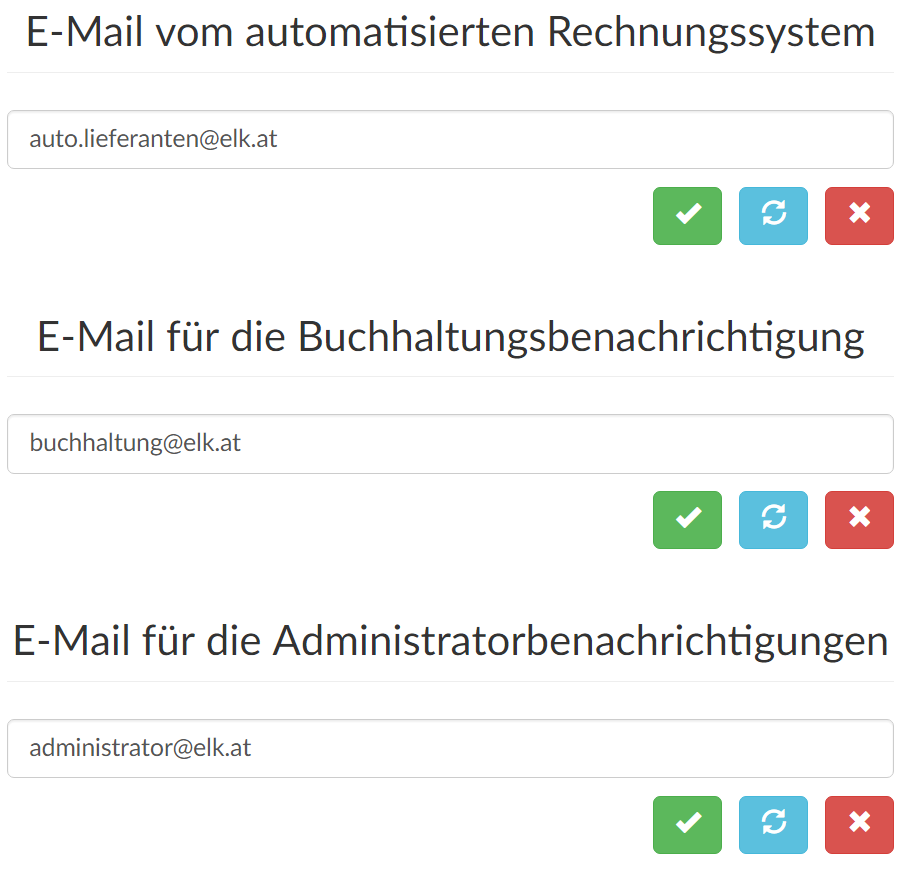
\includegraphics[width=15cm]{figures/emails.png}
    \label{fig:emailsverwaltung}
    \caption{E-Mail-Verwaltung}
\end{figure}ft. Auf diese E-Mail wird eine Benachrichtigung gesendet, wenn sich ein neuer Lieferant anmeldet.
\begin{figure}[!h]
    \centering
    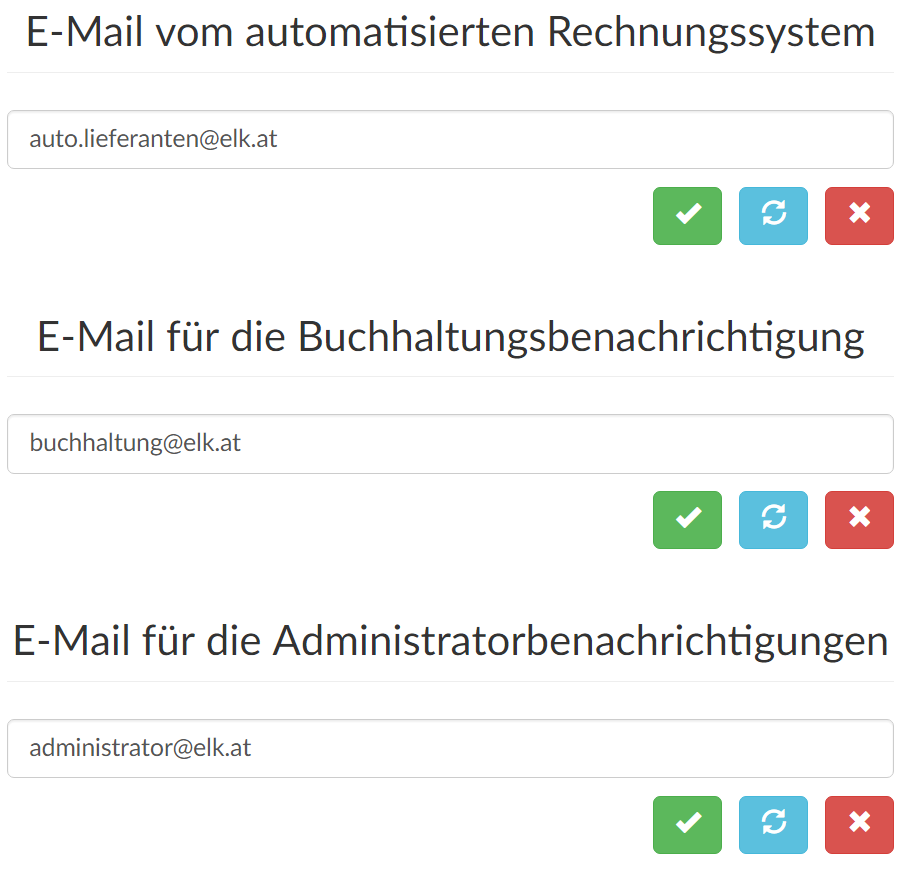
\includegraphics[width=15cm]{figures/emails.png}
    \label{fig:emailsverwaltung}
    \caption{E-Mails-Verwaltung}
\end{figure}
\chapter{Testfälle}
Nach Fertigstellung der Anwendung wurden von jedem Teammitglied Testfälle für seinen Aufgabenbereich verfasst (siehe \ref{tab:Testfaelle}). Die Testung erfolgte dann vom jeweilig anderen Projektpartner, um mögliche Denkfehler, die bereits beim Entwickeln auftraten und sich auch durch die Erstellung der Tests zogen, zu verhindern. Bei der Anwendung wurden die kritischen Teile der Anwendung genauestens getestet (Login, Rechnung holen, Registrieren, Rechnung hochladen). Die anderen Funktionen wurden aufgrunddessen, dass diese nicht so komplex sind, nur grundlegend getestet. 

\chapter{Ergebnisse \& Ausblick}
Das Projekt \glqq Webplattform für Rechnungserfassung\grqq{} wurde im Rahmen der Diplomarbeit erfolgreich fertiggestellt.

Das Projekt-Team hat alle MUSS- und OPTIONALEN Ziele erreicht und sogar noch vereinzelte Ziele, die für ein besseres Benutzen der Plattform förderlich sind, realisiert. Trotz Änderungen, die kurz vor dem Fertigstellungs-Termin von Herrn Ferkl angegeben wurden, ist das Projekt abgeschlossen und kann vollständig verwendet werden.

Wenn die Arbeit auf dem Webserver der Firma ELK GmbH lauffähig ist, entlastet sie die Buchhaltung der Firma ELK GmbH und ist so ein voller Erfolg. Falls im Laufe der Benutzung noch etwaige Fehler zum Vorschein kommen, werden diese außerhalb der Diplomarbeit korrigiert und zählen so nicht mehr zur eigentlichen Diplomarbeit. 
\chapter{Fazit}
Zusammenfassend hat es dem Projektteam viel Spaß gemacht hat, diese Arbeit zu erstellen und dann umzusetzen. Während des Projektes stieß das Team oftmals an seine Grenzen. Jedoch durch Zusammenhalt und gemeinsame Arbeitsstunden konnte jede Problematik gelöst werden. Interessant war auch die neue Anwendung von dem Framework Laravel, das vom Team zuvor noch nie benutzt wurde. Gott sei Dank verfügt dieses Framework über eine ausführliche Dokumentation, woraus die beiden viel erfahren konnten. Die größten Schwierigkeiten gab es mit der Oracle-Datenbank, denn diese wurde im Unterricht kurz durchgenommen, jedoch konnte diese lange Zeit nicht auf den Computern, auf welchen die Anwendung entwickelt wurde, installiert werden, wodurch das Projekt erst spät startete.

Das Projekt zeigte dem Team auf, dass es schwierig ist, die Zeit gut einzuteilen und dass man größere Puffer bei den Meilenstein-Vereinbarungen einrechnen sollte.

Auch die erstmalige Erfahrung, ein Projekt in Kooperation mit einer Firma abzuwickeln, war sehr interessant und oftmals eine große Umstellung gegenüber einem schulinternen Projekt, denn in der Schule fragte man einfach schnell die Professoren, wie diese es haben möchten. Doch bei Projekten mit einer echten Firma herrscht ein reger E-Mail-Verkehr, in dem alle Fragen gestellt und bestmöglich beantwortet werden.

Alles im allen sind Florian Mold und Michael Vogler sehr zufrieden mit dem Verlauf ihrer Arbeit und konnten viel neues Wissen und neue Erfahrungen sammeln.

%Römische Nummerierung im Inhaltsverzeichnis
\renewcommand\thechapter{\Roman{chapter}} 
%Beginnen der Römischen Nummerierung bei I
\setcounter{chapter}{0} 
%bindet Literatur-, Abbildungs-, Tabellen- und Abkürzungsverzeichnis ein
%
% Literatur-, Abbildungs-, Tabellen- und Abkürzungsverzeichnis
%


% Literaturverzeichnis ===>>>> siehe DA.bib
\nocite{*} %alle Einträge aus DA.bib werden übernommen, auch diese, die nicht im Text vorkommen
\bibliographystyle{babunsrt} %sortiere Verzeichnis nach Reihenfolge im Text
\bibliography{DA} %erstelle Verzeichnis





% erstellt ein File mit der Liste aller Bilder (Endung: *.lof)
\listoffigures



% erstellt ein File mit der Liste aller Tabellen (Endung: *.lot)
\listoftables

\renewcommand\lstlistlistingname{Quellcodeverzeichnis} 
\lstlistoflistings 

\chapter{Quellcodeverweise}
\markboth{Quellcodeverweise}{}
\begin{bfscript}{Platzhalter}

\item [Login-Methode\label{logincode}] CD "/Rechnungsplattform/app/Controllers/LoginController.php"

\item [Registrier-Methode \label{regiscode}] CD "/Rechnungsplattform/app/Controllers/LoginController.php"

\item [Rechung holen-Methode \label{holencode}] CD "/Rechnungsplattform/app/Controllers/AccountingController.php"

\item [Passwort vergessen-Methode \label{vergessencode}] CD "/Rechnungsplattform/app/Controllers/LoginController.php"

\item [Rechnung hochladen-Methode \label{hochladencode}] CD "/Rechnungsplattform/app/Controllers/SupplierController.php"

\item [Datenbank-Synchronisations-Funktion \label{datenbanksynchronisationcode}] CD "/Rechnungsplattform/app/Console/Commands/SynchronizeDatabase.php"

\item [Datenbank-Synchronisations-Fehlerbehanldungs-Funktion \label{datenbanksynchronisationfehlerbehandlungcode}] CD "/Rechnungsplattform/app/Console/Commands/SynchronizeDatabase.php"

\end{bfscript}

\chapter{Abkürzungsverzeichnis}
%\thispagestyle{empty}
\markboth{Abkürzungsverzeichnis}{}
%
\begin{bfscript}{Platzhalter}
% Hier die verwendeten Abkürzungen einfügen !
\item[XML] Extensible Markup Language
\item[HTML] Hypertext Markup Language
\item[PHP] Hypertext Preprocessor
\item[SQL] Structured Query Language
\item[PDF] Portable Document Format
\item[IDE] Integrierte Entwicklungsumgebung
\item[HTTP] Hyper Text Transfer Protocol
\item[AJAX] Asynchronous JavaScript and XML
\item[LATEX] Lamport TeX
\item[CLI] Command Line Interface
\end{bfscript}
%

%Beginn des Anhangs
\begin{appendix}
\chapter{Anhang}
\section{Pflichtenheft}
\subsection{Projektbeschreibung}

Die Firma ELK wünscht sich ein System mit dem es möglich sein soll,
die Eingangsrechnungen der Lieferanten über eine Internetplattform
zu managen. Die Lieferanten sollen sich anmelden können und so im
Stande sein, ihre Rechnungen als PDF mit Beschlagwortung hochzuladen.
Sobald eine Rechnung hochgeladen wurde, wird die Buchhaltung der Firma
ELK via E-Mail darüber informiert. Die Buchhaltung kann über eine
eigene Internetplattform die Rechnungen herunterladen. Zugestellt
werden sie in Form einer E-Mail, wie diese aussieht, folgt weiter unten.
Die ganzen Vorgänge auf den Plattformen sollen mitprotokolliert werden,
wie zum Beispiel das Löschen einer Rechnung, Holen einer Rechnung oder wenn jemand
eine Benachrichtigung sendet.


\subsection{Zielbestimmungen}


\subsubsection{Muss-Ziele}
\begin{itemize}
\item Lieferantenplattform 

\begin{itemize}
\item Der Lieferant kann sich mit seiner Lieferantennummer registrieren
und wartet bis er vom Administrator freigeschaltet wird. Nach der
Freischaltung erhält er eine Benachrichtigung per E-Mail. 
\item Nur freigeschaltete Lieferanten können sich auf der Plattform anmelden. 
\item Der Lieferant muss angemeldet sein, um Rechnungen hochladen zu können. 
\item Rechnung hochladen: 

\begin{itemize}
\item Rechnungen im PDF-Format hochladen 
\item Beschlagwortung der Rechnungen, vordefinierte Form muss ausgefüllt
werden. Die Vorgaben für die Beschlagwortung werden von der Firma
ELK an uns genauestens übergeben. 
\end{itemize}
\end{itemize}
\item Buchhaltungsplattform: 

\begin{itemize}
\item Es gibt einen gemeinsamen Buchhaltungsbenutzer, wodurch man das Holen
der Rechnungen nicht für die einzelnen Nutzer mitprotokollieren kann. 
\item Wenn der Buchhaltungsbenutzer angemeldet ist, kann dieser: 

\begin{itemize}
\item Rechnungen herunterladen 
\item Rechnungen einsehen 
\item Rechnungen löschen 
\end{itemize}
\item Pro Rechnung wird eine E-Mail versendet. 
\item E-Mail: 

\begin{itemize}
\item Sie enthält die Rechnung als PDF und die Beschlagwortung als XML-Datei,
welche von Herr Ferkl vorgegeben wird. 
\item Dies wird durch einen von uns generierten Job erledigt. 
\end{itemize}
\end{itemize}
\item Administratoransicht: 

\begin{itemize}
\item Der Administrator kann das Intervall festlegen, wann die Passwörter
geändert werden müssen. 

\begin{itemize}
\item Das Intervall kann für Lieferanten und Buchhalter getrennt festgelegt
werden. 
\end{itemize}
\item Der Administrator kann die Lieferanten freischalten sowie auch sperren. 
\item Nur der Administrator kann den Buchhaltungsbenutzer erstellen. 
\item Der Administrator kann \textbf{\small{}KEINE} Rechnungen holen! 
\item Der Administrator kann Kriterien für Passwörter festlegen. Wenn Passwortkriterien
geändert werden, müssen alle Benutzer bei der nächsten Anmeldung ihr
Passwort ändern.
\end{itemize}
\item Loggen: 

\begin{itemize}
\item Lieferanten: 

\begin{itemize}
\item Wenn ein Lieferant eine Rechnung hochlädt 
\item Wenn ein Lieferant einer Rechnung eine Benachrichtigung hinzufügt. 
\item Ob eine Benachrichtigung hinzugefügt oder eine Rechnung hochgeladen
wird, wird jeweils in einer eigenen Logdatei mitgeschrieben. 
\item Ein Eintrag in der Logdatei sieht so aus: {[}Datum{]}-{[}Uhrzeit{]}-{[}Lieferantnummer{]}-{[}Rechnungsnummer{]} 
\end{itemize}
\item Buchhaltung: 

\begin{itemize}
\item Wann und welche Rechnung gelöscht oder geholt wird. 
\item Beide Fälle, gelöscht oder geholt, werden in einer eigenen Logdatei
gespeichert. 
\item Ein Eintrag im Log sieht so aus: {[}Datum{]}-{[}Uhrzeit{]}-{[}Rechnungsnummer{]} 
\end{itemize}
\item Lieferant freischalten/sperren: 

\begin{itemize}
\item Wenn ein Lieferant freigeschaltet oder gesperrt wird. 
\item Ein Eintrag im Log sieht so aus: {[}Datum{]}-{[}Uhrzeit{]}-{[}Lieferantennummer{]}-{[}freigeschaltet/gesperrt{]} 
\end{itemize}
\end{itemize}
\end{itemize}

\subsubsection{Optionale-Ziele}
\begin{itemize}
\item Lieferantenplattform: 

\begin{itemize}
\item Lieferant sieht, welche seiner Rechnungen noch nicht geholt wurden,
kann aber diese nicht mehr ändern. 
\item Falls der Lieferant eine fehlerhafte Rechnung hochlädt, kann er die
Buchhaltung durch Drücken eines Benachrichtungsbuttons informieren. 

\begin{itemize}
\item Die Benachrichtigung erfolgt via E-Mail. In der E-Mail stehen die
Rechnungsnummer und eine Beschreibung des Fehlers. 
\item In der Datenbank wird die Beschreibung des Fehlers zur Rechnung hinzugespeichert. 
\item Buchhaltungsplattform: Falls eine Beschreibung hinzugefügt wurde,
wird diese gekennzeichnet und die Buchhaltung kann sich die Beschreibung
des Fehlers durchlesen.
\end{itemize}
\end{itemize}
\end{itemize}

\subsubsection{Nicht-Ziele}
\begin{itemize}
\item Die bestehende automatische Rechnungsverwaltung der Firma ELK soll
nicht verändert werden. 
\item Die Lieferantendatenbank der Firma ELK besteht schon und soll nicht
verändert werden, sondern nur mit unserer Datenbank synchronisiert
werden. 
\item Nach Versenden der E-Mail, welche die Rechnung und die Metadaten enthält,
ist der Aufgabenbereich unserer Diplomarbeit beendet. 
\end{itemize}

\subsection{Produkteinsatz}


\subsubsection{Anwendungsbereich}

Das Endprodukt wird verwendet, um den Rechnungsaustausch zwischen den
Lieferanten und der Firma ELK elektronisch abzuwickeln, um so die Arbeit
der Buchhaltung der Firma ELK zu minimieren.


\subsubsection{Zielgruppen}

Das System wird hauptsächlich von der Buchhaltung und den Lieferanten
verwendet.


\subsubsection{Betriebsbedingungen}
\begin{itemize}
\item Für den Betrieb der Software ist ein Internetzugang für den Lieferanten
sowie für die Buchhaltung der Firma ELK notwendig. 
\item Der Zugriff auf den Webserver, wo die Webseite gespeichert ist und
die Datenbank muss gewährleistet sein. 
\end{itemize}

\subsection{Produktumgebung}


\subsubsection{Software}

Auf dem Zielsystem wird nur ein Browser gebraucht, da die Software
auf einem Server läuft.


\subsubsection{Hardware}

Zur Verwendung unseres Produktes benötigt man einen Webserver und
einen Rechner mit Internetzugang.


\subsubsection{Produktschnittstelle}
\begin{itemize}
\item Das Produkt wird in das bereits vorhandene automatische Rechnungsverwaltungssystem
der Firma ELK eingegliedert. 
\item Unser Produkt erhält täglich die Lieferantenstammdaten des bereits
bestehenden Oracle Datenbanksystems der Firma ELK. 
\end{itemize}

\subsection{Produktfunktionen}


\subsubsection{Lieferantenansicht}
\begin{enumerate}
\item Der Lieferant registriert sich. 
\item Er wartet bis er freigeschaltet wird und wird durch ein E-Mail über
die Freischaltung informiert. 
\item Lieferant kann sich anmelden. 
\item Lieferant kann eine Rechnung nach der anderen hochladen. 
\item Falls eine Rechnung fehlerhaft ist, kann der Lieferant die Buchhaltung
benachrichtigen. 
\item Kann seine offenen Rechnungen ansehen. 
\end{enumerate}

\subsubsection{Buchhaltungsansicht}
\begin{enumerate}
\item Der Buchhaltungsbenutzer kann sich anmelden. 
\item Buchhaltungsbenutzer kann eine Rechnung einsehen. 
\item Buchhaltungsbenutzer kann Rechnungen via E-Mail holen. 
\item Buchhaltungsbenutzer kann Rechnungen löschen. 
\end{enumerate}

\subsubsection{Administratoransicht}
\begin{enumerate}
\item Administrator kann das Intervall für die Passwortänderung für Lieferanten
und Buchhaltungsmitarbeiter getrennt festlegen. 
\item Administrator kann Lieferanten freischalten, sowie sperren. 
\item Der Administrator kann den Buchhaltungsbenutzer erstellen. 
\item Administrator kann Kriterien für das Passwort festlegen. 
\end{enumerate}

\subsection{Benutzeroberfläche}

Das Design sollte dem von der Homepage der Firma ELK (\url{http://www.elk.at},
Stand: September 2015) ähneln.


\subsection{Qualitäts-Zielbestimmungen}
\begin{itemize}
\item Das Produkt sollte für jeden Benutzer nach einer Einschulung verwendbar
sein. 
\item Durch unseren passwortgesicherten Zugang wird sichergestellt, dass
keine privaten Daten der Firma ELK an die Öffentlichkeit gelangen. 
\end{itemize}

\subsection{Globale Testszenarien und Testfälle}
\begin{itemize}
\item Ein Lieferant kann sich ohne Freischaltung nicht anmelden. 
\item Beim Hochladen der Rechnung muss jedes Feld ausgefüllt werden und
eine PDF angehängt sein. 
\item Das Passwort muss den vorgegebenen Kriterien entsprechen. (Sonderzeichen,
Zahlen, Groß-Kleinbuchstaben) 
\item Das Passwort muss nach dem angegebenen Intervall geändert werden. 
\item Nach dem Hochladen einer Rechnung erhält die Buchhaltung eine E-Mail
und die Rechnung wird in der Buchhaltungsansicht angezeigt. 
\item Der von uns generierte Job, welcher die XML erstellt und XML und PDF
per E-Mail versendet, funktioniert einwandfrei. 
\item Unsere E-Mail wird von der automatischen Rechnungsverwaltung angenommen
und weiterverarbeitet 
\item Es sollen Prüfungen sowie Korrekturmöglichkeiten geben, damit bei
einem Absturz keine inkonsistenten Daten weggeschrieben werden. 
\end{itemize}

\subsection{Entwicklungsumgebung}


\subsubsection{Software}
\begin{itemize}
\item Das Produkt wird auf dem Betriebssystem Windows 10 entwickelt. 
\item Das Produkt wird auf Google Chrome und Mozilla Firefox getestet. 
\item Als Entwicklungsumgebung kommt JetBRAINS PhpStorm Version 9.xx zum
Einsatz. 
\item Zum lokalen Testen wird der Apache-Server von XAMPP verwendet mit
der Datenbankumgebung von Oracle. 
\end{itemize}

\subsubsection{Hardware}
\begin{itemize}
\item Zum Entwickeln werden zwei Laptops eingesetzt. 
\end{itemize}

\subsubsection{Entwicklungsschnittstelle}

Die bereits bestehende Datenbank der Firma ELK dient als Schnittstelle
für unsere neu hinzukommende Datenbank.


\subsection{Ergänzungen}

Die zum Entwickeln notwendige Oracle-Lizenz bekommen wir von der Firma
ELK zur Verfügung gestellt. 

\newpage
\subsection{Use-Case-Diagramm}
\begin{figure}[h]
\centering
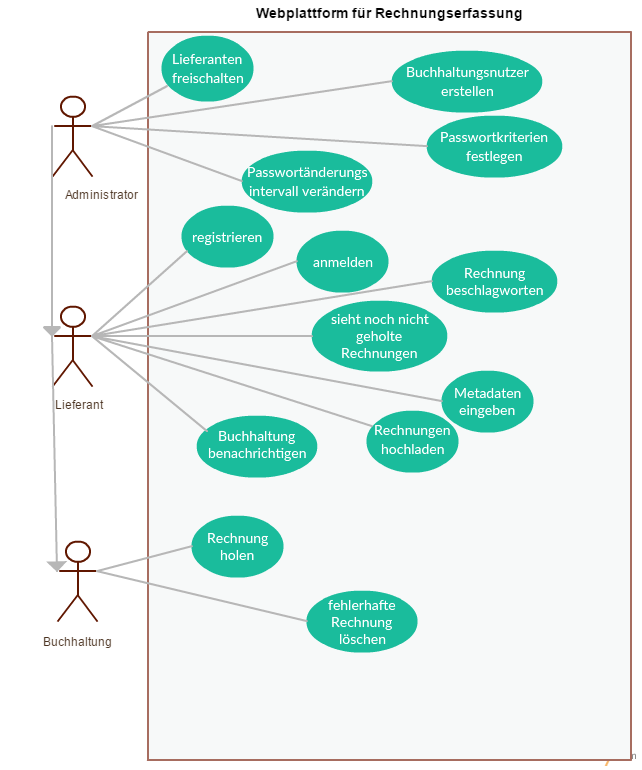
\includegraphics[width=13cm]{figures/Use-Case-Diagramm}
\caption{Use-Case-Diagramm}
\end{figure}

\newpage
\subsection{Quellen}

Dieses Pflichtenheft ist angelehnt an diese Webseite: \\
 \url{http://www.infrasoft.at/downloads/Anleitung_zum_Pflichtenheft.pdf}


\subsection{Unterschriften}

Alle beteiligten Personen sind mit dem Pflichtenheft einverstanden
und das Projekt soll laut diesem Pflichtenheft entstehen. Für weitere
Fragen steht Herr Ferkl zur Verfügung.

\vspace{2cm}

\begin{labeling}{00.00.0000}
\item [{%
\begin{tabular}{>{\raggedright}p{7cm}}
\dotfill{}\tabularnewline
Michael Vogler\tabularnewline
\end{tabular}\hfill{}%
\begin{tabular}{>{\raggedright}p{7cm}}
\dotfill{}\tabularnewline
Florian Mold\tabularnewline
\end{tabular}}]~
\item [{\vspace{2cm}
}]~
\item [{\vspace{2cm}
}]~
\item [{%
\begin{tabular}{>{\raggedright}p{7cm}}
\dotfill{}\tabularnewline
Christopher Ferkl\tabularnewline
\end{tabular}\hfill{}%
\begin{tabular}{>{\raggedright}p{7cm}}
\dotfill{}\tabularnewline
Alexander Mestl\tabularnewline
\end{tabular}}]~\end{labeling}


\chapter{Testfälle}
\begin{longtable}[h]{| c | p{3.7cm} | p{3.8cm} | l | l | l | c |}
\caption{Testfälle}\label{tab:Testfaelle}\\ 
\toprule
* & Testfall & Erwartetes Resultat & Ersteller & Tester & Ergebnis \\          
\midrule
\endfirsthead
\caption[]{Testfälle \small(Fortsetzung)}\\
\toprule
* & Testfall & Erwartetes Resultat & Ersteller & Tester & Ergebnis \\
\midrule
\endhead
\midrule
\endfoot 
\bottomrule
\endlastfoot 
\hline
1 & Registrieren eines neuen Lieferanten mit Testdaten. \textbf{Benutzername:} Testlieferant \textbf{E-Mail:} eigene E-Mail \textbf{Passwort:} Secret!1 \textbf{Lieferantennummer:} 80536 & Lieferanten-Benutzer wird in der Datenbank erstellt. Die Buchhaltung sowie der Lieferant erhalten eine E-Mail, dass der Registriervorgang erfolgreich war. & Mold Florian & Vogler Michael & OK \\ \hline

2 & Ein Eingabefeld beim Registrieren nicht ausgefüllt. z.B.: Benutzername & Entsprechende Fehlermeldung wird angezeigt & Mold Florian  & Vogler Michael & OK \\ \hline

3 & Eingabe eines Passworts, dass nicht den Kriterien oder der Länge entspricht. z.B.: 123 & Eine Fehlermeldung mit den geforderten Passwortkriterien und der vorausgesetzten Länge wird ausgegeben. & Mold Florian & Vogler Michael & OK \\ \hline

4 & Absetzen einer Passwort-Vergessen Anfrage mit einer E-Mail, die in der Plattform enthalten ist. z.B.: v.m.diplomarbeit @gmail.com & Der Tester erhält eine E-Mail, die einen Link zum Zurücksetzen des Passworts beinhaltet. & Mold Florian & Vogler Michael & OK \\ \hline

5 & Link in der E-Mail abrufen. Dann gelangt der Benutzer auf die Passwort-Vergessen Seite. Danach wird ein neues Passwort eingegeben und das Formular abgeschickt & Das Passwort wird in der Datenbank verändert und der Benutzer gelangt zurück zur Login-Seite & Mold Florian & Vogler Michael & OK \\ \hline

6 & Login-Versuch mit folgenden Daten \textbf{E-Mail:} supplier@gmail.com \textbf{Passwort:} secret & Benutzer wird auf die Lieferantenseite weitergeleitet. & Mold Florian & Vogler Michael & OK \\ \hline

7 & Login-Versuch mit folgenden Daten \textbf{E-Mail:} adminmail@gmail.com \textbf{Passwort:} secret & Benutzer wird auf die Administratorseite weitergeleitet. & Mold Florian &  Vogler Michael & OK \\ \hline

8 & Login-Versuch mit folgenden Daten \textbf{E-Mail:} accounting@gmail.com  \textbf{Passwort:} secret & Benutzer wird auf die Buchhaltungsseite weitergeleitet. & Mold Florian &  Vogler Michael & OK \\ \hline

9 & Vergessen eines Eingabefeldes bei einem Login-Versuch. z.B.: Passwortfeld & Dem Benutzer wird eine Fehlermeldung angezeigt, die ihn darauf hinweist alles auszufüllen. & Mold Florian & Vogler Michael & OK \\ \hline

10 & In der Lieferantenansicht einer Rechnung eine Benachrichtigung hinzufügen. & Die Benachrichtigung kann direkt nach dem Absenden betrachtet werden und die Buchhaltung erhaelt eine E-Mail, die die Benachrichtigung aufweist. Weiters wird dem Rechnungseintrag in der Datenbank die Benachrichtigung hinzugefügt. & Mold Florian & Vogler Michael & OK \\ \hline

11 & In der Buchhaltungsansicht eine Rechnung löschen. & Die Rechnung soll nicht mehr angezeigt werden und in der Datenbank beim entsprechenden Eintrag soll der Status auf "deleted" gesetzt sein. Ein Eintrag in der "deleted.log" Datei wird zusaetzlich erstellt. Dem Benutzer wird eine Erfolgsmeldung angezeigt. & Mold Florian &  Vogler Michael & OK \\ \hline

12 & In der Buchhaltungsansicht eine Rechnung "holen". & In der Datenbank wird der Status der Rechnung auf "taken" gesetzt. Desweiteren wird die Rechnung nicht mehr angezeigt und die Rechnung sowie die Metadaten per E-Mail an die computerunterstützte Buchhaltung weitergeleitet. Zusätzlich wird ein Eintrag in der "taken.log" Datei erstellt. & Mold Florian &  Vogler Michael & OK \\ \hline

13 & In der Buchhaltungsansicht alle Rechnungen gleichzeitig verarbeiten. & In der Datenbank wird der Status aller Rechnungen, die keine Benachrichtigung haben auf "taken" gesetzt. Die Rechnungen sollen auch nicht mehr in der Tabelle angezeigt werden und die computerunterstützte Buchhaltung der Firma ELK Fertighaus GmbH erhält die Rechnungen und die Metadaten per E-Mails. Zusätzlich werden Einträge für jede Rechnung in der "taken.log" Datei erstellt. & Mold Florian & Vogler Michael & OK \\ \hline

14 & In der Buchhaltungsansicht alle Rechnungen gleichzeitig verarbeiten. & In der Datenbank wird der Status aller Rechnungen, die keine Benachrichtigung haben auf "taken" gesetzt. Die Rechnungen sollen auch nicht mehr in der Tabelle angezeigt werden und die computerunterstützte Buchhaltung der Firma ELK Fertighaus GmbH erhält die Rechnungen und die Metadaten per E-Mails. Zusätzlich werden Einträge für jede Rechnung in der "taken.log" Datei erstellt. & Mold Florian & Vogler Michael & OK \\ \hline

15 & Passwort ändern beim \textbf{Benutzer:} Testuser \textbf{Passwort:} secret. Das alte Passwort soll falsch eingegeben werden. & Dem Benutzer wird eine Fehlermeldung angezeigt, dass das aktuelle Passwort nicht richtig war. & Mold Florian & Vogler Michael & OK \\ \hline

16 & Passwort ändern beim \textbf{Benutzer:} Testuser \textbf{Passwort:} secret. Neues Passwort entspricht nicht den geforderten Passwortkriterien. & Dem Benutzer wird eine Fehlermeldung mit den vorausgesetzten Passwortkriterien angezeigt. & Mold Florian & Vogler Michael & OK \\ \hline

17 & Passwort ändern beim \textbf{Benutzer:} Testuser \textbf{Passwort:} secret. Passwort soll erfolgreich geändert werden. Dazu das aktuelle Passwort eingeben (secret) und neues Passwort festlegen (Secret!1) & Das Passwort wird in der Datenbank verändert und der Benutzer gelangt zurück zu seiner Hauptseite. & Mold Florian & Vogler Michael & OK \\ \hline

18 & Passwort ändern beim \textbf{Benutzer:} Testuser \textbf{Passwort:} secret. Das beiden neuen Passwörter, die eingegeben wurden, sollen nicht übereinstimmen. & Dem Benutzer wird eine Fehlermeldung angezeigt, dass die beiden Passwörter nicht übereinstimmen. & Mold Florian & Vogler Michael & OK \\ \hline

19 & In der Lieferansicht eine Rechnung hochladen. Dazu eine PDF-Datei in das Feld ziehen und dazu die Metadaten angeben. & Rechnungseintrag mit den Metadaten wird in der Datenbank erstellt, zusätzlich wird die PDF-Datei auf dem Dateisystem abgelegt. Dem Lieferanten wird anschließend die Rechnung in der "Rechnungen-Tabelle" angezeigt. & Vogler Michael & Mold Florian & OK \\ \hline

20 & Ein Eingabefeld beim Rechnung-hochladen vergessen. z.B.: Betrag, PDF-Datei & Der Benutzer bekommt eine Fehlermeldung angezeigt, dass alle Felder ausgefüllt werden müssen, bevor der Vorgang abgeschlossen werden kann. & Vogler Michael & Mold Florian & OK \\ \hline

21 & Als Administrator anmelden. & Auf der Startseite des Administratorbereichs werden die bestehenden Daten (Anzahl der Lieferanten, der freigeschalteten Lieferanten, der neuen Lieferanten und der offenen Rechnungen) angezeigt. & Vogler Michael & Mold Florian & OK \\ \hline

22 & Die Lieferantenverwaltung aufrufen. & Es werden alle registrierten und freigeschalteten Lieferanten in der dazugehörigen Tabelle angezeigt. & Vogler Michael & Mold Florian & OK \\ \hline

23 & Ein Lieferant registriert sich auf der Plattform. & Dieser Lieferant wird in der Lieferantenverwaltung in einer dritten Tabelle angezeigt. Dort werden die Lieferanten nur angezeigt, solange Sie noch nie freigeschaltet wurden. & Vogler Michael & Mold Florian & OK \\ \hline

24 & Auf den grünen Button mit dem Häkchen klicken. & Der Lieferant wird freigeschaltet. Er wird mithilfe einer E-Mail über die Freischaltung benachrichtigt. Ab diesen Zeitpunkt kann er sich auf der Plattform anmelden und Rechnungen hochladen. & Vogler Michael & Mold Florian & OK \\ \hline

25 & Auf den roten Button mit dem Schloss klicken. & Der Lieferant wird gesperrt. Er wird mithilfe einer E-Mail über die Sperrung benachrichtigt und kann sich ab diesen Zeitpunkt nicht mehr auf der Plattform anmelden. & Vogler Michael & Mold Florian & OK \\ \hline

26 & Bei den Lieferanten auf den roten Button mit dem Kreuz klicken. & Man muss das Löschen des Lieferanten bestätigen und dann wird dieser mit einer E-Mail über den Löschvorgang benachrichtigt. Seine Rechnungen bleiben weiter bestehen. & Vogler Michael & Mold Florian & OK \\ \hline

27 & Die Buchhalter-Seite aufrufen. & Die gesperrten und freigeschalteten Buchhalter werden in der richtigen Tabelle angezeigt. & Vogler Michael & Mold Florian & OK \\ \hline

28 & Einen Buchhalter erstellen und eines der Felder leer lassen. & Eine rote Box mit einer Fehlermeldung erscheint. & Vogler Michael & Mold Florian & OK \\ \hline

29 & Einen Buchhalter freischalten, sperren oder löschen. & Dieser wird mit einer E-Mail benachrichtigt. & Vogler Michael & Mold Florian & OK \\ \hline

30 & Die Passwortkriterien für einen Buchhalter ändern. & Es ist möglich die Passwortkriterien für die Buchhalter, Lieferanten und Administratoren getrennt festzulegen. & Vogler Michael & Mold Florian & OK \\ \hline

31 & Neue Passwortkriterien festlegen. & Beim nächsten Mal anmelden müssen die Benutzer deren Passwort an die neuen Kriterien anpassen. & Vogler Michael & Mold Florian & OK \\ \hline

32 & Das Intervall, in welchem das Passwort geändert werden muss, ändern. & Beim Anmelden wird auf das neue Intervall überprüft. & Vogler Michael & Mold Florian & OK \\ \hline

33 & Standort ändern, dazu auf den blauen Button mit dem Stift klicken. & Es ist nur die Bezeichnung des Standortes änderbar. Die Nummer ist nur lesbar. & Vogler Michael & Mold Florian & OK \\ \hline

34 & Ein Standort anlegen und alle Felder ausfüllen. & Es wird eine Erfolgsnachricht am Beginn der Seite angezeigt. & Vogler Michael & Mold Florian & OK \\ \hline

35 & Standort löschen. & Es ist keine Möglichkeit verfügbar, mit welcher ein Standort gelöscht werden kann, da ansonst Daten bei vorhandenen Rechnungen fehlen könnten. & Vogler Michael & Mold Florian & OK \\ \hline

36 & Beim Hinzufügen von einer neuen Währung ein Feld nicht befüllen. & Ein rotes Kästchen mit einer Fehlermeldung erscheint am Beginn der Seite. & Vogler Michael & Mold Florian & OK \\ \hline

37 & Währung ändern. & Nach dem Speichern der geänderten Währungen werden die aktuellen Daten angezeigt. & Vogler Michael & Mold Florian & OK \\ \hline

38 & Währung probieren zu Löschen. & Währungen kann man nicht löschen, da diese vielleicht bei vorhandenen Rechnungen gebraucht werden. & Vogler Michael & Mold Florian & OK \\ \hline

39 & Seite der Rechnungsarten aufrufen. & Alle Rechnungsarten werden angezeigt. & Vogler Michael & Mold Florian & OK \\ \hline

40 & Bei den Rechnungsarten wird der ausgeschriebene Name und das dazugehörige Kürzel geändert und alle beiden Felder sind ausgefüllt. & Eine grüne Bestätigungsbenachrichtigung erscheint und die Daten sind aktualisiert. & Vogler Michael & Mold Florian & OK \\ \hline

41 & Eine neue Rechnungsart hinzufügen, aber nicht alle Felder ausfüllen und auf den grünen Button mit dem Plus klickt. & Eine rote Fehlermeldung erscheint am Beginn der Seite. & Vogler Michael & Mold Florian & OK \\ \hline

42 & Die E-Mails für das automatische Rechnungssystem, die Buchhaltungsbenachrichtigungen und die Administratorbenachrichtigungen sind eingetragen. Für eine dieser drei ist keine E-Mail in der Datenbank vorhanden. & Es erscheint über diesem Textfeld eine rote Warnung. & Vogler Michael & Mold Florian & OK \\ \hline

43 & Eine der drei E-Mails ändern und dabei die Textbox leer lassen. & Es erscheint eine rote Fehlermeldung am Anfang der Seite. & Vogler Michael & Mold Florian & OK \\ \hline
\end{longtable}

\clearpage
\section{Stundenaufzeichnung}
In folgendem Abschnitt finden Sie die aufgewendeten Stunden der jeweiligen Projektpartner.
\subsection{Florian Molds Stunden}
\begin{longtable}[h]{| c | p{11.6cm} | l | l |}
\caption{Stundenaufzeichnung Florian}\label{tab:stundenaufzeichnung}\\ 
\toprule
* & Tätigkeit & Dauer (h) & Datum \\
\midrule
\endfirsthead
\caption[]{Stundenaufzeichnung Florian \small(Fortsetzung)}\\
\toprule
* & Tätigkeit & Dauer (h) & Datum \\
\midrule
\endhead
\midrule
\endfoot 
\bottomrule
\endlastfoot 
\hline

1 & 1. Besprechung mit Auftraggeber & 2 & 22.04.2015 \\ \hline

2 & 1. Besprechung mit Herrn Mestl & 1,25 & 25.04.2015 \\ \hline

3 & 2. Besprechung mit Auftraggeber & 1,5 & 29.05.2015 \\ \hline

4 & 2. Besprechung mit Herrn Mestl & 1 & 19.06.2015 \\ \hline

5 & Pflichtenheft schreiben & 6 & 28.08.2015 \\ \hline

6 & Pflichtenheft schreiben & 6 & 28.08.2015 \\ \hline

7 & Design mit Herrn Mestl besprochen & 2 & 20.09.2015 \\ \hline

8 & Einlesen in Oracle Datenbanktechnologie & 3 & 25.09.2015 \\ \hline

9 & Designentwicklung der Login-Seite in HTML & 2 & 02.10.2015 \\ \hline

10 & Designentwicklung der Lieferanten-Seite in HTML & 2,5 & 05.10.2015 \\ \hline

11 & EWA: Einführung in wissenschaftliches Arbeiten & 3 & 05.10.2015 \\ \hline

12 & Designentwicklung der Buchhalter-Seite in HTML & 3 & 10.10.2015 \\ \hline

13 & ER-Modell Entwurf der Datenbank & 1,5 & 15.10.2015 \\ \hline

14 & 3. Besprechung mit Herrn Mestl & 0,4 & 16.10.2015 \\ \hline

15 & Auswahl des geeigneten Entwicklerframeworks für das Projekt & 2 &  20.10.2015 \\ \hline

16 & Installation des Laravel-Frameworks & 1 &  30.10.2015 \\ \hline

17 & Einarbeiten in das Laravel-Framework & 3 & 02.11.2015 \\ \hline

18 & EWA: Einführung in wissenschaftliches Arbeiten & 3 & 03.11.2015 \\ \hline

19 & Bereits vorhandene Seiten in die Laravel Template Engine integrieren. & 4 & 27.11.2015 \\ \hline

20 & EWA: Einführung in wissenschaftliches Arbeiten & 3 & 10.11.2015 \\ \hline

21 & 4. Besprechung mit Herrn Mestl & 0,3 & 20.11.2015 \\ \hline

22 & EWA: Einführung in wissenschaftliches Arbeiten & 4 & 15.12.2015 \\ \hline

23 & Installation des Oracle Express Edition Datenbanksystems & 2 & 12.01.2016 \\ \hline

24 & Login-Funktionalität für Lieferanten umsetzen & 3 & 20.01.2016 \\ \hline

25 & 5. Besprechung mit Herrn Mestl & 0,5 & 29.01.2015 \\ \hline

26 & Registrierung für Lieferanten realisiert & 3 & 29.01.2016 \\ \hline

27 & Verfassen eines groben Inhaltsverzeichnisse für die Diplomarbeit & 2 &  29.01.2016 \\ \hline

28 & Registrierung fertiggestellt & 1 & 30.01.2016 \\ \hline

29 & Implementierung einer Passwort-Vergessen Form & 2 & 31.01.2016 \\ \hline

30 & Passwortkriterien müssen beim Regisitrieren beachtet werden & 2 & 01.02.2016 \\ \hline

31 & Passwort-Vergessen Mail-Benachrichtigung funktioniert &  3 & 02.02.2016 \\ \hline

32 & Beim Login wird für jede Benutzergruppe eine Session erstellt & 1 & 03.02.2016 \\ \hline

33 & Rechnungen werden aus der Datenbank ausgelesen und in die Tabellen geschrieben & 2 & 03.02.2016 \\ \hline

34 & Login-Fehler behoben + Erfolgs- / Fehlermeldungen & 1 & 03.02.2016 \\ \hline

35 & Passwort-Ändern Buchhalter, Lieferant und Administrator & 3 & 05.02.2016 \\ \hline

36 & Passwort-Ändern Fehlerbehebung & 0,5 & 08.02.2016 \\ \hline

37 & 404 Fehlerseite erstellt & 1 & 08.02.2016 \\ \hline

38 & Prüfen ob z.B.: Benutzer die Lieferantenseite betrachten darf & 1 & 08.02.2016 \\ \hline

39 & Rechnung löschen & 1 & 08.02.2016 \\ \hline

40 & Rechnung im Browser betrachten & 0,5 & 08.02.2016 \\ \hline

41 & Abfrage ob die Rechnung wirklich gelöscht werden soll & 0,5  & 09.02.2016 \\ \hline

42 & Metadaten für jede einzelne Rechnung ausgelesen um im zugehörigen Modal angezeigt & 1 & 09.02.2016\\ \hline

43 & Benachrichtigung für jede Rechnung ausgelesen & 0,5 & 09.02.2016 \\ \hline

44 & Logging Funktionaltität begonnen & 1 & 09.02.2016 \\ \hline

45 & Design-Verbesserung der Backend-Seite & 1 & 09.02.2016 \\ \hline

46 & Weitere Verbesserung der Backend Seite & 2 & 10.02.2016 \\ \hline

47 & Mail wird bereits mit Rechnung als Anhang versendet & 1 & 10.02.2016 \\ \hline

48 & Zusätzlich zur Benachrichtigungsspeicherung in der Datenbank wird die Benachrichtigung als Mail an die Buchhaltung versendet. & 1,5 & 11.02.2016 \\ \hline

49 & Das Intervall, wann das Passwort geändert werden muss, greift beim Login vom Administrator, Buchhalter und Lieferant & 2,5 & 12.02.2016 \\ \hline

50 & XML-Datei lässt sich bereits generieren, allerdings fehlen noch die richtigen Elemente & 1 & 12.02.2016 \\ \hline

51 & Die Mails die absgesendet werden müssen, werden nicht sofort verschickt, sondern in eine Warteschlange geschoben und später versendet. Dies verbessert die Response-Zeit der Anwendung, da die Benutzer nicht warten müssen, bis die Mail verschickt ist, sondern sie können gleich weiterarbeiten & 2 & 12.02.2016 \\ \hline

52 & Direkt nach dem Versenden kann der Lieferant, seine Benachrichtigungen betrachten. & 0,5 & 12.02.2016 \\ \hline

53 & 403 Fehlerseite erstellt & 0,5  & 12.02.2016 \\ \hline

54 & Code-Dokumentation der Loginklasse, Buchhaltungsklasse, Lieferantenklasse, Methodsklasse zum selbst erstellten Programmcode & 2 & 12.02.2016 \\ \hline

55 & Die Registrierform wird nach der Registrierung geleert, vorher blieben alle Werte darin enthalten & 0,5 & 13.02.2016 \\ \hline

56 & Code-Dokumentation der HTML-Seiten, Datenbanktabellen, Migrations & 3 & 13.02.2016 \\ \hline

57 & Fehlerbehebung bei der Lieferantenansicht. & 0,25 & 13.02.2016 \\ \hline

58 & Anpassung der Login-Seite für mobile Desktops & 1,5 & 13.02.2016 \\ \hline

59 & Anpassung der Buchhaltungs- / Lieferantenseite für mobile Desktops & 1 & 14.02.2016 \\ \hline

60 & Anpassung der Passwort-Vergessen und Passwort-Ändern Seite für mobile Desktops & 0,5 & 14.02.2016 \\ \hline

61 & Jeden Tag um 24 Uhr werden bereits geholte Rechnungen + xmls gelöscht & 1 & 16.02.2016 \\ \hline

62 & Sicherung des Standes der kompletten Datenbank wird jeden Tag um 24 Uhr durchgeführt & 1 & 16.02.2016 \\ \hline

63 & Tabellen der Buchhaltungsseite / Lieferantenseite und Administratorseite für mobile Auflösungen optimiert & 1 & 17.02.2016 \\ \hline

64 & Ablaufdiagramm für den Login erstellt & 1 & 18.02.2016 \\ \hline

65 & Ablaufdiagramm für die Registrierung erstellt & 1 & 18.02.2016 \\ \hline

66 & Ablaufdiagramm für das Rechnung holen erstellt & 1 & 18.02.2016 \\ \hline

67 & Ablaufdiagramm für den Passwort-Vergessen erstellt & 1 & 18.02.2016 \\ \hline

68 & EWA: Einführung in wissenschaftliches Arbeiten & 3 & 23.02.2016 \\ \hline

69 & 3. Besprechung mit Auftraggeber & 2 & 24.02.2016 \\ \hline

70 & 6. Besprechung mit Herrn Mestl & 1 & 26.02.2016 \\ \hline

71 & XML-Datei mit den richtigen Elementen, Attributen und Werten wird erstellt & 1,5 & 24.02.2016 \\ \hline

72 & Logging Funktion für alle geforderten Funktionen implementiert & 2 & 25.02.2016 \\ \hline

73 & Erweiterung der Datenbank um einen Rechnungsstatus wie z.B.: gelöscht, geholt, ... & 0,5 & 25.02.2016 \\ \hline

74 & Kleine Fehlerbehebung beim Benachrichtigung anzeigen / senden & 0,5 & 25.02.2016 \\ \hline

75 & Alle offenen Rechnungen ohne Benachrichtigung lassen sich von der Buchhaltung gleichzeitig holen & 1,5 & 27.02.2016 \\ \hline

76 & Überprüfung, ob eine zu holende Rechnung bereits von einem anderen Buchhaltungsbenutzer geholt wurde & 1 & 27.02.2016 \\ \hline

77 & Fehlerbehebung bei den Datatables. Diese werden nun automatisch vergrößert/verkleinert wenn sich die Auflösung der Seite ändert. Nachdem die Seite aktualisiert wurde, kommt man wieder auf den richtigen Tab beim Tabcontrol, wo man zuvor war. & 2,5 & 28.02.2016 \\ \hline

78 & Rechnung können nun nicht mehr von allen Benutzern gelesen werden, sondern nur noch von authentifizierten Anwendern. & 2 & 28.02.2016 \\ \hline

79 & Verfassen der Einleitung der Diplomarbeit & 2 & 29.02.2016 \\ \hline

80 & Schreiben des ersten Kapitels & 4 & 29.02.2016 \\ \hline

81 & Umsetzung des aktuellen Standes der Stunden in das Dokument & 1,5 & 29.02.2016 \\ \hline

82 & Beginn des Verfassens von Testfällen & 2 & 29.02.2016 \\ \hline

83 & Vervollständigen der Testfälle & 2 & 31.02.2016 \\ \hline

84 & Beschreiben der Funktionen (Registrieren, Login) & 3 & 01.03.2016 \\ \hline

85 & Beschreiben der Funktionen (Rechnung holen, Passwort vergessen & 2 & 02.03.2016 \\ \hline

86 & Beschreiben von Laravel & 3 & 04.03.2016 \\ \hline

87 & Beschreiben von Composer, PHP, XML & 3 & 05.03.2016 \\ \hline

88 & Beschreiben von Latex, Phpstorm & 2 & 06.03.2016 \\ \hline

89 & Beschreiben von SQL Developer, XAMPP & 2 & 08.03.2016 \\ \hline

90 & Beschreiben von Chrome, Firefox & 1 & 10.03.2016 \\ \hline

91 & Beschreiben von Dropbox, Texmaker & 2 & 13.03.2016 \\ \hline

92 & Einfügen eines Bildes des Datenbankmodells + Beschreibung dieser & 3 & 14.03.2016 \\ \hline

93 & Einfügen einer Gender-Erklärung in das Dokument & 0,5 & 15.03.2016 \\ \hline

94 & Übersetzen der Einleitung ins Englische & 1,5 & 18.03.2016 \\ \hline

95 & Testfälle von Michael getestet & 4 & 19.03.2016 \\ \hline

96 & Testfälle allgemein verfasst & 0,5 & 20.03.2016 \\ \hline

97 & Einrichtung der Anwendung bei ELK Fertighaus GmbH & 2,5 & 21.03.2016 \\ \hline

98 & E-Mail wird auch an Administrator versendet, wenn sich ein Lieferant registriert & 2,5 & 26.03.2016 \\ \hline

\end{longtable}

\subsection{Michael Voglers Stunden}
\begin{longtable}[h]{| c | p{11.6cm} | l | l |}
\caption{Stundenaufzeichnung Michael}\label{tab:stundenaufzeichnung_michael}\\ 
\toprule
* & Tätigkeit & Dauer (h) & Datum \\
\midrule
\endfirsthead
\caption[]{Stundenaufzeichnung Michael \small(Fortsetzung)}\\
\toprule
* & Tätigkeit & Dauer (h) & Datum \\
\midrule
\endhead
\midrule
\endfoot 
\bottomrule
\endlastfoot 
\hline

1 & A\underline{\ }01 - Besprechung mit Herrn Ferkl & 1,75 & 22.04.2015 \\ \hline
2 & B\underline{\ }01 - Besprechung mit Herrn Mestl & 1,25 & 25.04.2015 \\ \hline
3 & A\underline{\ }02 - Besprechung mit Herrn Ferkl & 1,25 & 29.05.2015 \\ \hline
4 & B\underline{\ }02 - Besprechung mit Herrn Mestl & 1 & 19.06.2015 \\ \hline
5 & Pflichtenheft schreiben & 6 & 28.08.2015 \\ \hline
6 & Pflichtenheft für Abgabe überarbeiten & 1,5 & 13.09.2015 \\ \hline
7 & Design mit Herrn Mestl besprechen & 2,75 & 20.09.2015 \\ \hline
8 & Grobes Design der Login-Seite zeichnen & 1 & 21.09.2015 \\ \hline
9 & Freifach EWA -> Latex und Regeln lernen & 3 & 05.10.2015 \\ \hline
10 & in Oracle einlesen & 3 & 13.10.2015 \\ \hline
11 & Datenbankmodel erstellen & 1,5 & 15.10.2015 \\ \hline
12 & B\underline{\ }03 - Besprechung mit Herrn Mestl & 0,4 & 16.10.2015 \\ \hline
13 & Datenbankmodel überarbeiten & 1 & 29.10.2015 \\ \hline
14 & Freifach EWA -> Latex und Regeln lernen & 4 & 03.11.2015 \\ \hline
15 & Freifach EWA -> Latex und Regeln lernen & 3 & 10.11.2015 \\ \hline
16 & B\underline{\ }04 - Besprechung mit Herrn Mestl & 0,3 & 20.11.2015 \\ \hline
17 & Freifach EWA -> Latex und Regeln lernen & 3 & 15.12.2015 \\ \hline
18 & Admin-Backend neu gestalten & 4 & 21.01.2016 \\ \hline
19 & Laravel ORM einlesen & 3,5 & 24.01.2016 \\ \hline
20 & Datenbank in Laravel umsetzen & 3,25 & 24.01.2016 \\ \hline
21 & Seed-Daten für Datenbank erstellen & 1,75 & 24.01.2016 \\ \hline
22 & Admin-Backend weiter machen & 2 & 28.01.2016 \\ \hline
23 & B\underline{\ }05 - Besprechung mit Herrn Mestl & 0,5 & 29.01.2016 \\ \hline
24 & Admin-Backend weiter machen & 2,25 & 29.01.2016 \\ \hline
25 & Laravel Controller einlesen & 1 & 29.01.2016 \\ \hline
26 & Admin-Backend weiter machen & 0,75 & 29.01.2016 \\ \hline
27 & Inhaltsverzeichnis erstellen & 2 & 29.01.2016 \\ \hline
28 & Methodenaufrufe in php und speziell in Laravel anschauen & 2 & 30.01.2016 \\ \hline
29 & Datenbankänderung überlegen; umsetzen und Seed-Daten hinzufügen (aufgrund der speicherbaren und änderbaren E-Mail der Buchhaltung und des Administrators -> nicht im Pflichtenheft angegeben) & 2 & 31.01.2016 \\ \hline
30 & Admin-Backend weitermachen (Lieferanten) & 2,5 & 31.01.2016 \\ \hline
31 & Datenbankänderung (Passwortkriterien -> Feld, für wen diese Kriterien gelten, hinzufügen) & 0,25 & 31.01.2016 \\ \hline
32 & Admin-Backend weiter machen (Passwortkriterien) & 1,5 & 31.01.2016 \\ \hline
33 & Laravel einlesen (Verwendung einer Form) & 0,5 & 31.01.2016 \\ \hline
34 & Admin-Backend weiter machen (Passwortkriterien auf Formelemente von Laravel umschreiben; Intervall updaten anfangen) & 1,5 & 31.01.2016 \\ \hline
35 & Admin-Backend weiter machen (Passwortkriterien -> Intervall update fertig gemacht) & 0,5 & 04.02.2016 \\ \hline
36 & Admin-Backend weiter machen (Passwortkriterien -> Kriterien updaten angefangen) & 1,5 & 05.02.2016 \\ \hline
37 & Lieferanten-Ansicht (Rechnung-hochladen weiter machen -> auf Laravel-Form umschreiben) & 1,75 & 08.02.2016 \\ \hline
38 & Lieferanten-Ansicht (Rechnung-hochladen weiter machen -> umschreiben auf Laravel-Form [Fehler suche]) & 1,75 & 09.02.2016 \\ \hline
39 & Lieferanten-Ansicht (Rechnung-hochladen weiter machen -> Rechnung wird in Datenbank angelegt; PDF hochladen fehlt noch) & 1,25 & 09.02.2016 \\ \hline
40 & Lieferanten-Ansicht (Rechnung-hochladen weiter machen -> Rechnung in Datenbank gespeichert und PDF in Verzeichnis abgelegt; PDF-Größe begrenzen -> probiert) & 3,25 & 10.02.2016 \\ \hline
41 & Admin-Backend weiter machen (USERID und Anzeigewerte der Informationen übergeben -> große Probleme) & 1,75 & 10.02.2016 \\ \hline
42 & Admin-Backend weiter machen (Design responive machen) & 0,25 & 10.02.2016 \\ \hline
43 & Admin-Backend weiter machen (Standorte entwerfen, Datatables inlineedit anschauen [funktioniert noch nicht]) & 3 & 10.02.2016 \\ \hline
44 & Admin-Backend weiter machen (Standorte entwerfen -> Funktionen funktionieren noch nicht) & 1 & 12.02.2016 \\ \hline
45 & Admin-Backend weiter machen (Standort hinzufügen und bearbeiten) & 3,5 & 12.02.2016 \\ \hline
46 & Admin-Backend weiter machen (Standort hinzufügen [Benachrichtigung ob funktioniert hat]) -> Standorte fuktionieren & 1,25 & 12.02.2016 \\ \hline
47 & Admin-Backend weiter machen (Währungen designen, hinzufügen und bearbeiten) & 0,5 & 12.02.2016 \\ \hline
48 & Admin-Backend weiter machen (Rückmeldung -> wenn gelungen; Fragen, ob Lieferant wirklich löschen) & 0,75 & 12.02.2016 \\ \hline
49 & Admin-Backend weiter machen (E-Mail für Buchhaltungssystem und Adminbetreffliches änderbar) & 1,5 & 12.02.2016 \\ \hline
50 & Admin-Backend weiter machen (Rechnungsarten designen und Funktionen anfangen) & 1,5 & 13.02.2016 \\ \hline
51 & Admin-Backend weiter machen (Rechnungsarten fertig designen und Funktionen ausprogrammieren) & 1,25 & 13.02.2016 \\ \hline
52 & Laravel einlesen (E-Mail versenden) & 0,5 & 13.02.2016 \\ \hline
53 & Admin-Backend weiter machen (E-Mail-Benachrichtigungen -> bei Buchhaltung- und Administrator-E-Mail) & 1,25 & 13.02.2016 \\ \hline
54 & Admin-Backend weiter machen (E-Mail-Benachrichtigungen -> bei Lieferanten-Verwaltung [wenn gesperrt/freigeschaltet/gelöscht werden]) & 2,5 & 13.2.2016 \\ \hline
55 & Admin-Backend weiter machen (Design responsive machen) & 0,5 & 14.02.2016 \\ \hline
56 & Laravel Cronjob anschauen & 1 & 14.02.2016 \\ \hline
57 & Teile vom Controller kommentieren & 0,5 & 14.02.2016 \\ \hline
58 & Laravel Cronjob anschauen; mit der Vorbereitung/Implementierung beginnen & 1,25 & 15.02.2016 \\ \hline
59 & Datenbanksynchronisation (CSV-Import suchen) & 1,75 & 16.02.2016 \\ \hline
60 & Datenbanksynchronisation (CSV-Import suchen; Implementierung beginnen) & 2,75 & 16.02.2016 \\ \hline
61 & Datenbanksynchronisation (CSV-Import nochmal verscuhen -> entscheiden, dass was anderes genommen wird) & 0,5 & 17.02.2016 \\ \hline
62 & Datenbanksynchronisation (neuen Import anschauen) & 1 & 18.02.2016 \\ \hline
63 & Datenbanksynchronisation (entschieden für Excel einlesen mit "laravel-excel") & 2,5 & 18.02.2016 \\ \hline
64 & Datenbanksynchronisation (fertigstellen) & 3 & 18.02.2016 \\ \hline
65 & Admin-Backend-Controller kommentieren & 1 & 22.02.2016 \\ \hline
66 & Freifach EWA -> Latex und Regeln lernen & 3 & 23.02.2016 \\ \hline
67 & A\underline{\ }03 - Besprechung mit Herrn Ferkl & 1,2 & 24.02.2016 \\ \hline
68 & B\underline{\ }06 - Besprechung mit Herrn Mestl & 1 & 26.02.2016 \\ \hline
69 & Lieferanten Rechnung-hochladen (loggen) & 0,5 & 28.02.2016 \\ \hline
70 & Admin-Backend Buchhaltungs-E-Mail änderbar machen & 1,75 & 29.02.2016 \\ \hline
71 & Lieferanten Rechnung-hochladen (Betrag und Steuerbetrag nicht negativ) & 1 & 29.02.2016 \\ \hline
72 & Admin-Backend (Buchhalter-Verwaltung -> Vorgaben änderten sich) & 1,5 & 01.03.2016 \\ \hline
73 & Admin-Backend weiter machen (Buchhalter-Verwaltung) & 2,25 & 01.03.2016 \\ \hline
74 & Admin-Backend weiter machen (Rechnungstypen -> Abkürzung hinzufügen und änderbar machen) & 1 & 03.03.2016 \\ \hline
75 & Admin-Backend weiter machen (Forms[Placeholder] und Texte ausbessern) & 0,5 & 03.03.2016 \\ \hline
76 & Admin-Backend weiter machen (validation bei allen Forms und alle Funktionen testen und überprüfen) & 2,25 & 03.03.2016 \\ \hline
77 & Dokumentation (Besprechungsprotokolle[Mestl und Ferkl] schreiben) & 3,5 & 05.03.2016 \\ \hline
78 & Dokumentation (Ablaufdiagramm für Rechnung-hochladen) & 1,25 &05.03.2016 \\ \hline
79 & Datenbank synchronisieren weiter machen & 1,75 & 06.03.2016 \\ \hline
80 & Oracle Datenbank läuft nicht mehr -> reparieren (erfolglos) & 1,25 & 07.03.2016 \\ \hline
81 & Oracle Datenbank läuft nicht mehr -> reparieren (Lösung suchen -> erfolglos) & 0,5 & 08.03.2016 \\ \hline
82 & Oracle Datenbank läuft nicht mehr -> reparieren (neu installieren -> erfolglos) & 0,75 & 09.03.2016 \\ \hline
83 & Oracle-Datenbank läuft nicht mehr -> reparieren (Problem -> Umgebungsvariable fehlt) -> funktioniert wieder & 0,75 & 10.03.2016 \\ \hline
84 & Datenbank synchronisieren weiter machen & 1,5 & 10.03.2016 \\ \hline
85 & Dokumentation (Latex alle Packages nachinstallieren) & 0,5 & 11.03.2016 \\ \hline
86 & Dokumenation (Ablaufdiagramm für Datenbank-Synchronisation) & 1,25 & 11.03.2016 \\ \hline
87 & Dokumentation (Aufgabenaufteilung; Laravel Excel; Bootstrap; jQuery) & 2,25 & 11.03.2016 \\ \hline
88 & Dokumentation (Ajax; HTML; JavaScript; CSS; Oracle SQL Developer) & 3,5 & 12.03.2016 \\ \hline
89 & Dokumenation (Testfälle; zitieren; Rechnung hochladen beginnen) & 6,5 & 14.03.2016 \\ \hline
90 & Dokumentation schreiben (zitieren; Rechnung hochladen fertigstellen); Datenbanksynchronisation; Rechnungsart kann nicht doppelt vorkommen & 4 & 16.03.2016 \\ \hline
91 & Admin-Bereich (Fehler ausgebessert; Datenbanksynchronisation fertigstellen) & 6,75 & 20.03.2016 \\ \hline
92 & Dataseeder umschreiben, dass richtige Werte in Anfangstabelle stehen & 0,25 & 20.03.2016 \\ \hline
93 & Rechnungsplattform auf Webserver der Firma ELK installiert (funktioniert nicht, haben veraltete Version) & 2,25 & 21.03.2016 \\ \hline
94 & Dokumentation(Datenbanksynchronisation fertigstellen; Protokolle mit Ferkl anfügen) & 3,25 & 22.03.2016 \\ \hline
95 & Dokumentation (Cronjob; Backend beginnen) & 3 & 23.03.2016 \\ \hline
96 & Dokumentation (Backend fertigstellen) & 1,5 & 24.03.2016 \\ \hline
97 & E-Mail-Versand anschauen (funktioniert nicht -> gelöst) & 0,5 & 24.03.2016 \\ \hline
98 & Zeiten von Besprechung nachtragen; Dokumentation (Arbeitsliste in Latex übernehmen; Fazit; Ergebnis) & 3,5 & 25.03.2016 \\ \hline
99 & Admin-Bereich testen -> Tests erfolgreich & 0,5 & 27.03.2016 \\ \hline
100 & Dokumentation noch einmal durchlesen und Fehler korrigieren & 1,5 & 27.03.2016 \\ \hline
101 & Dokumentation (Arbeitsliste vervollständigt) & 0,75 & 29.03.2016 \\ \hline

\end{longtable}
\chapter{Besprechungsprotokolle}
\section{Protokolle mit Betreuungslehrer}
Nachfolgend sind alle Protokolle, die bei Besprechungen mit unserem Betreuungslehrer Herrn Mestl entstanden sind, angeführt. Anhand dieser Mitschriften kann man erkennen, wieweit fortgeschritten unsere Arbeit in den einzelnen Zeiträumen war und ob und in wie fern wir die besprochenen Punkte erfüllt haben.
\begin{figure}[!h]
    \centering
    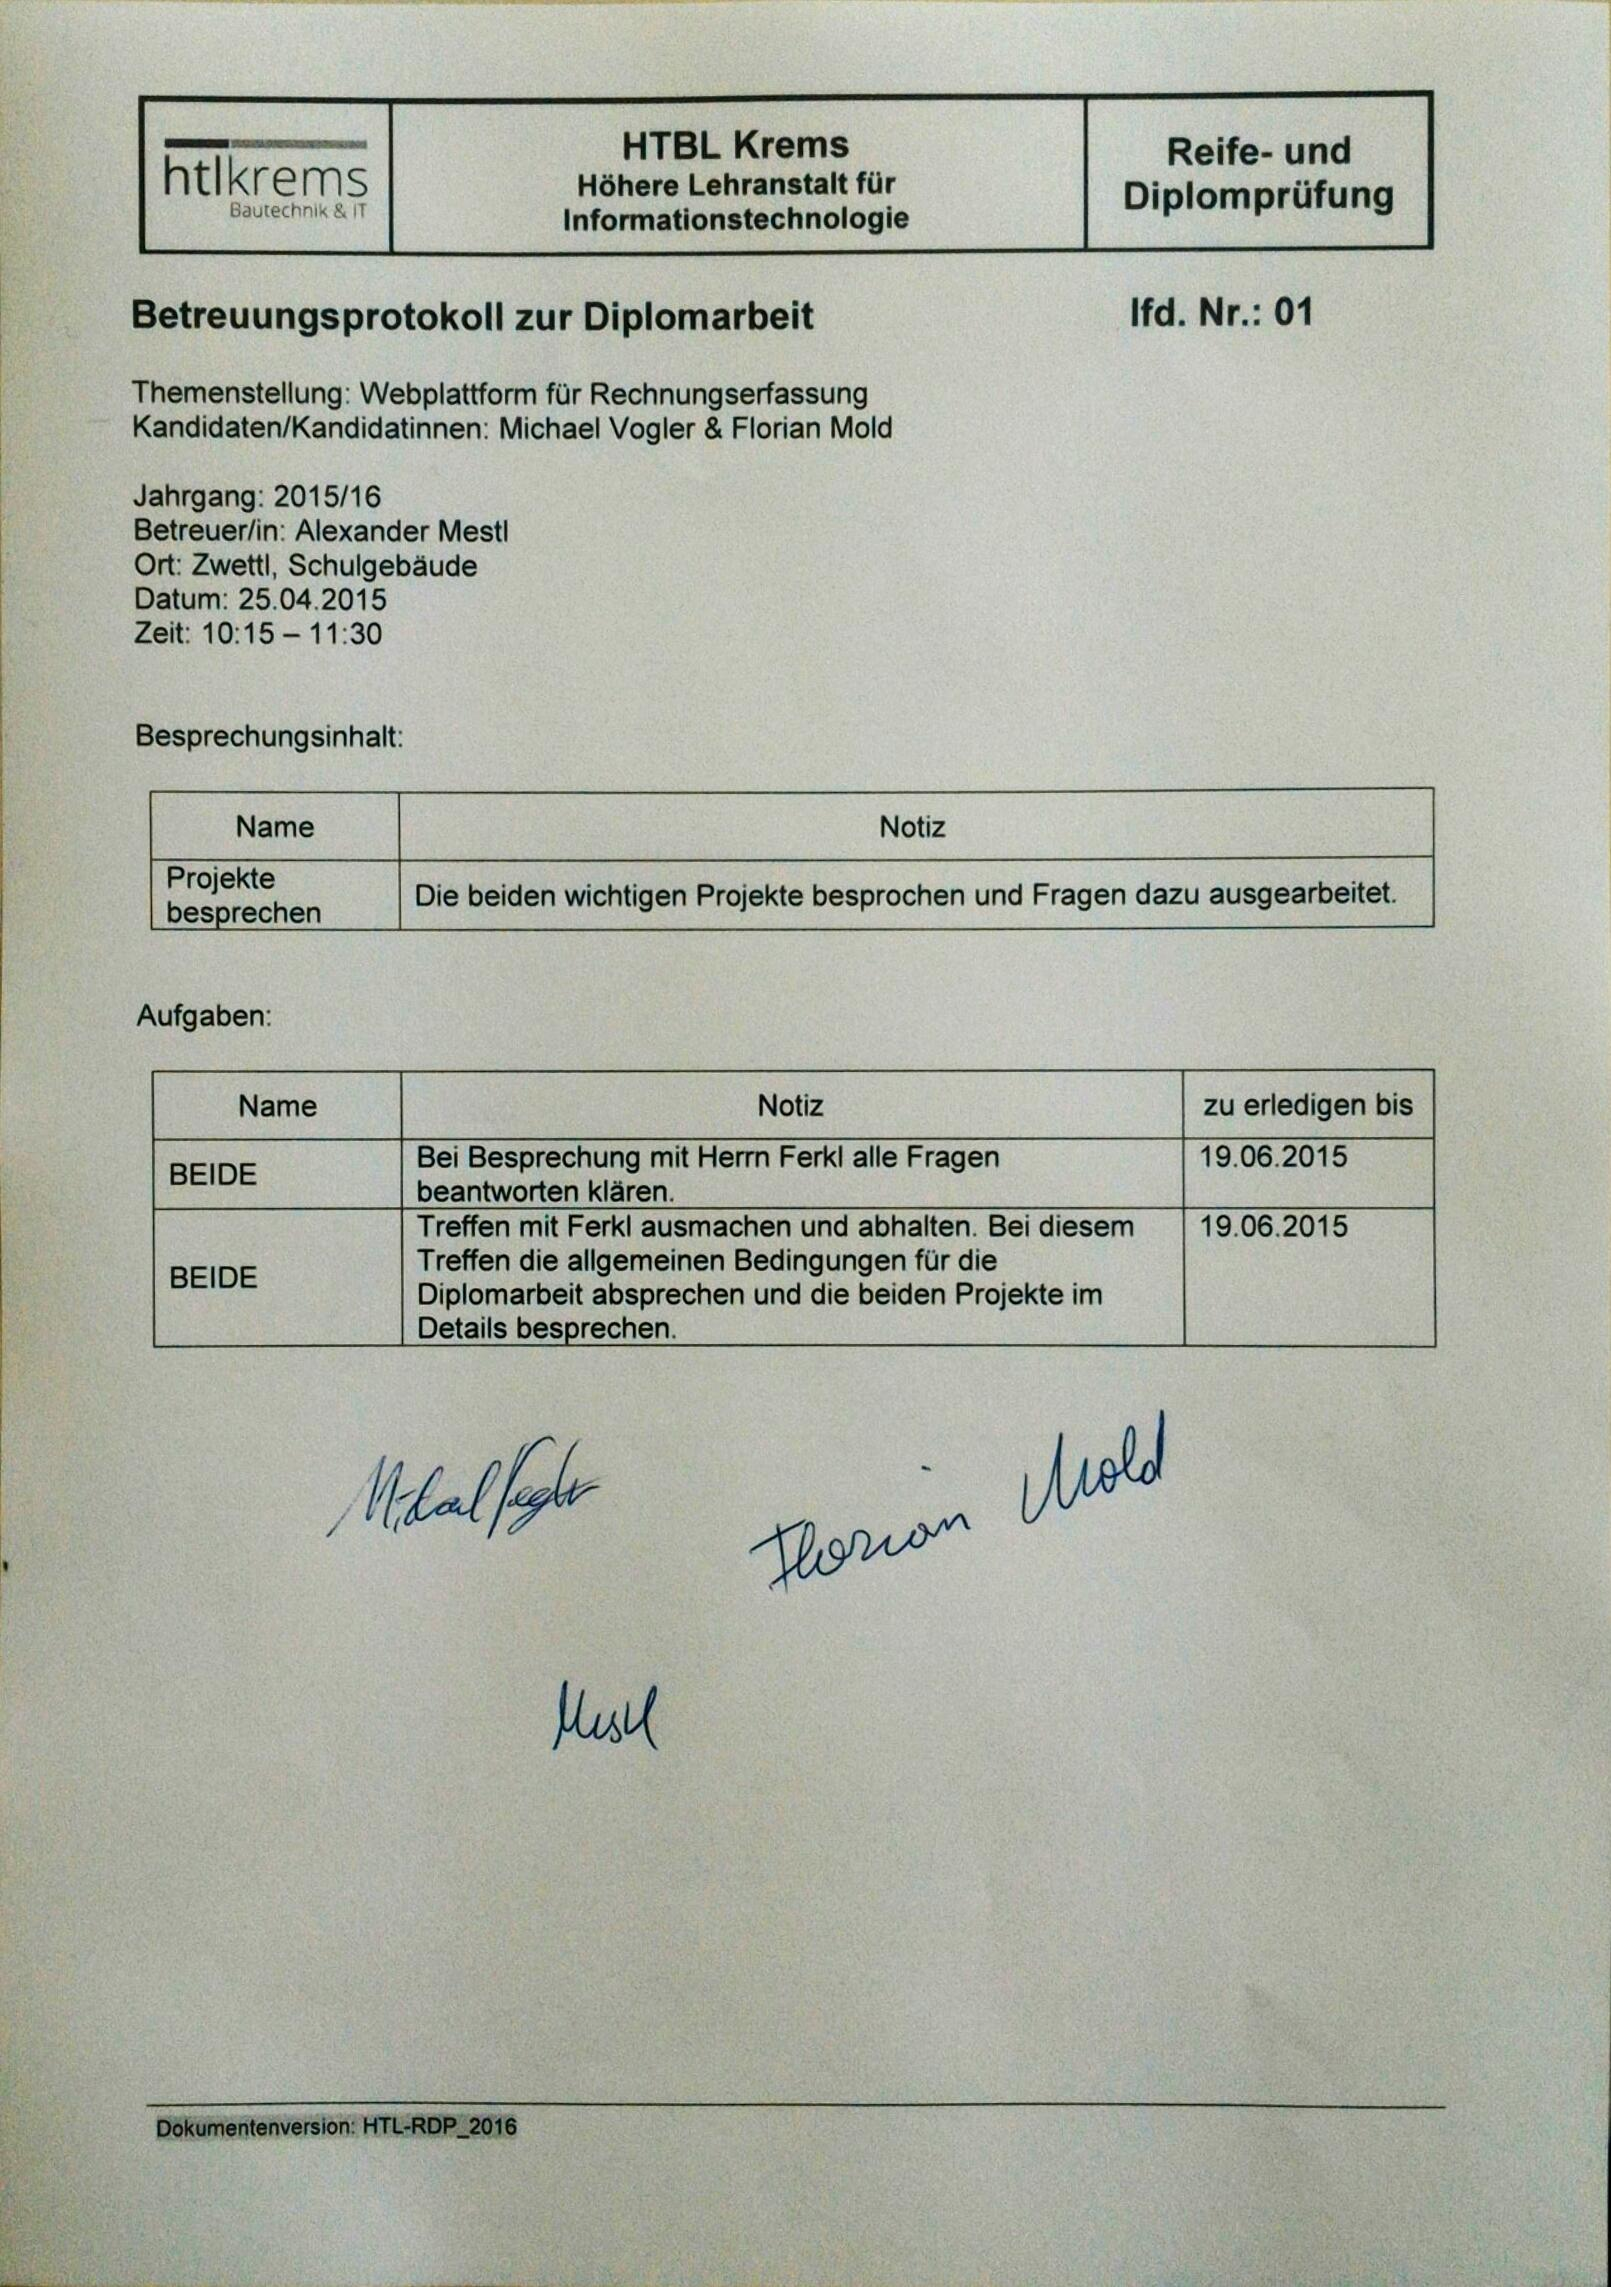
\includegraphics[width=13cm]{figures/Mestl_01.jpg}
    \label{fig:01_Protokoll_Betreuungslehrer}
    \caption{01 Protokoll mit Betreuungslehrer}
\end{figure}
\newpage
\begin{figure}[!h]
    \centering
    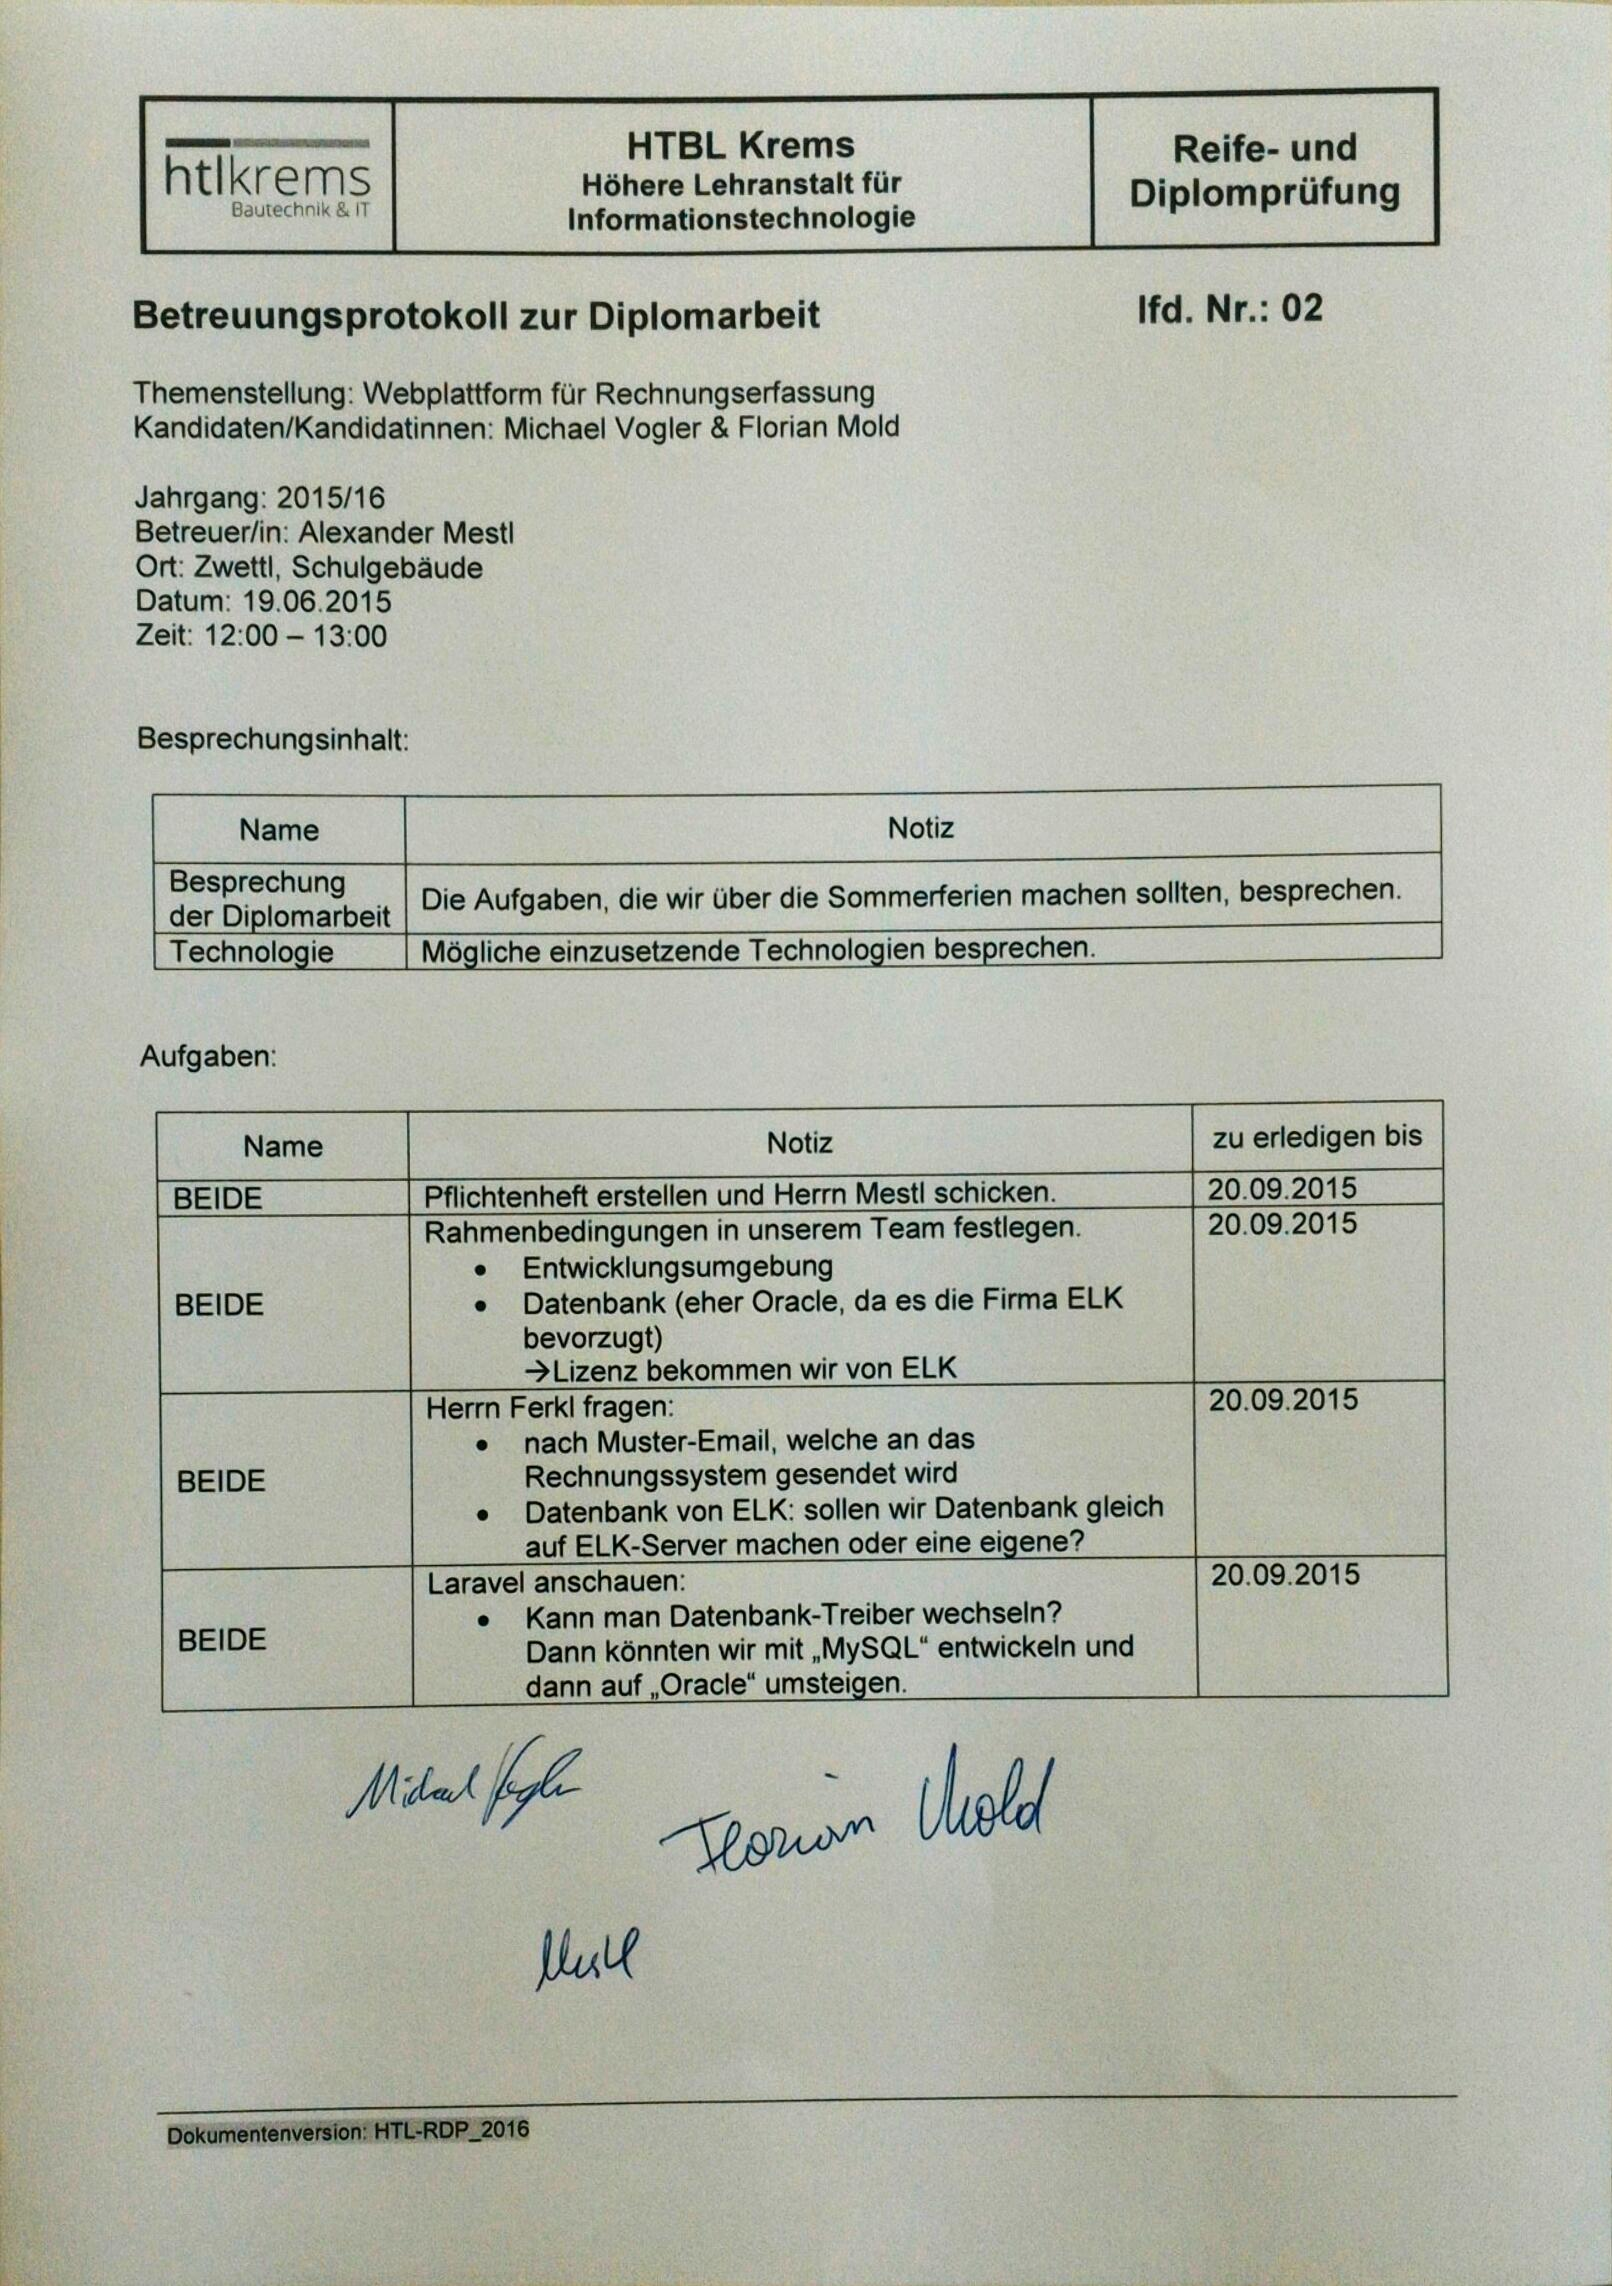
\includegraphics[width=13cm]{figures/Mestl_02.jpg}
    \label{fig:02_Protokoll_Betreuungslehrer}
    \caption{02 Protokoll mit Betreuungslehrer}
\end{figure}
\newpage
\begin{figure}[!h]
    \centering
    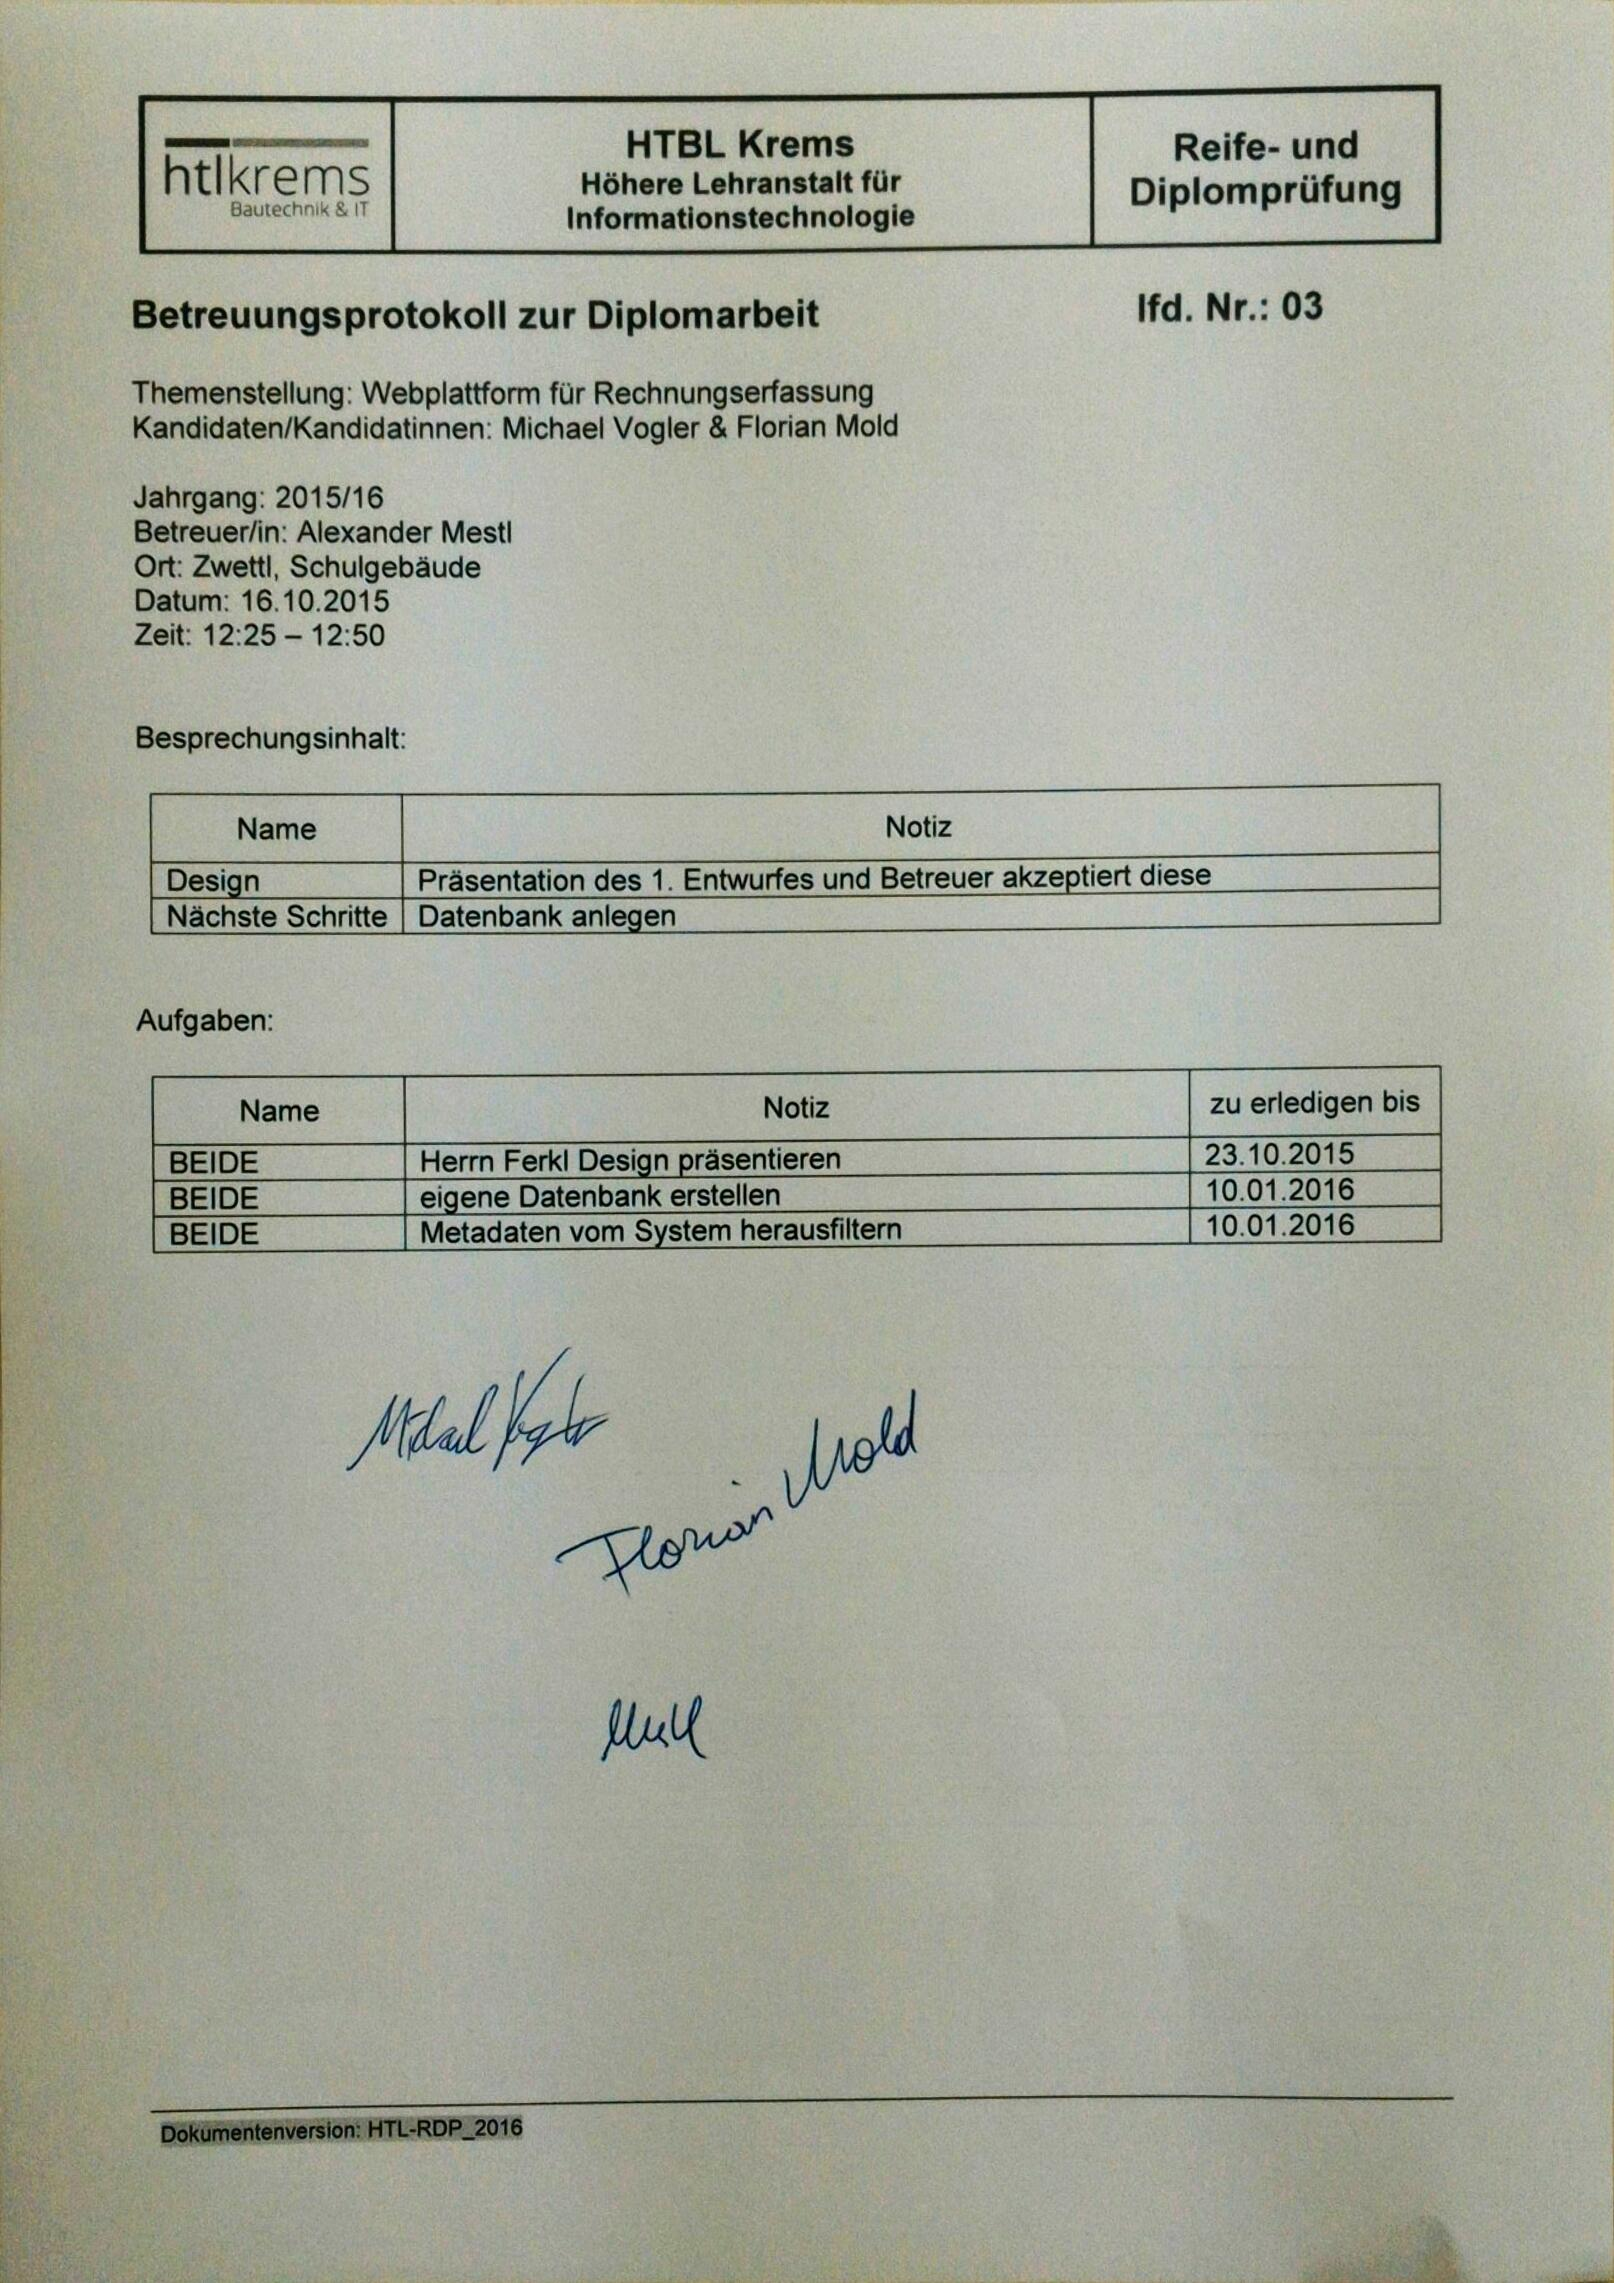
\includegraphics[width=13cm]{figures/Mestl_03.jpg}
    \label{fig:03_Protokoll_Betreuungslehrer}
    \caption{03 Protokoll mit Betreuungslehrer}
\end{figure}
\newpage
\begin{figure}[!h]
    \centering
    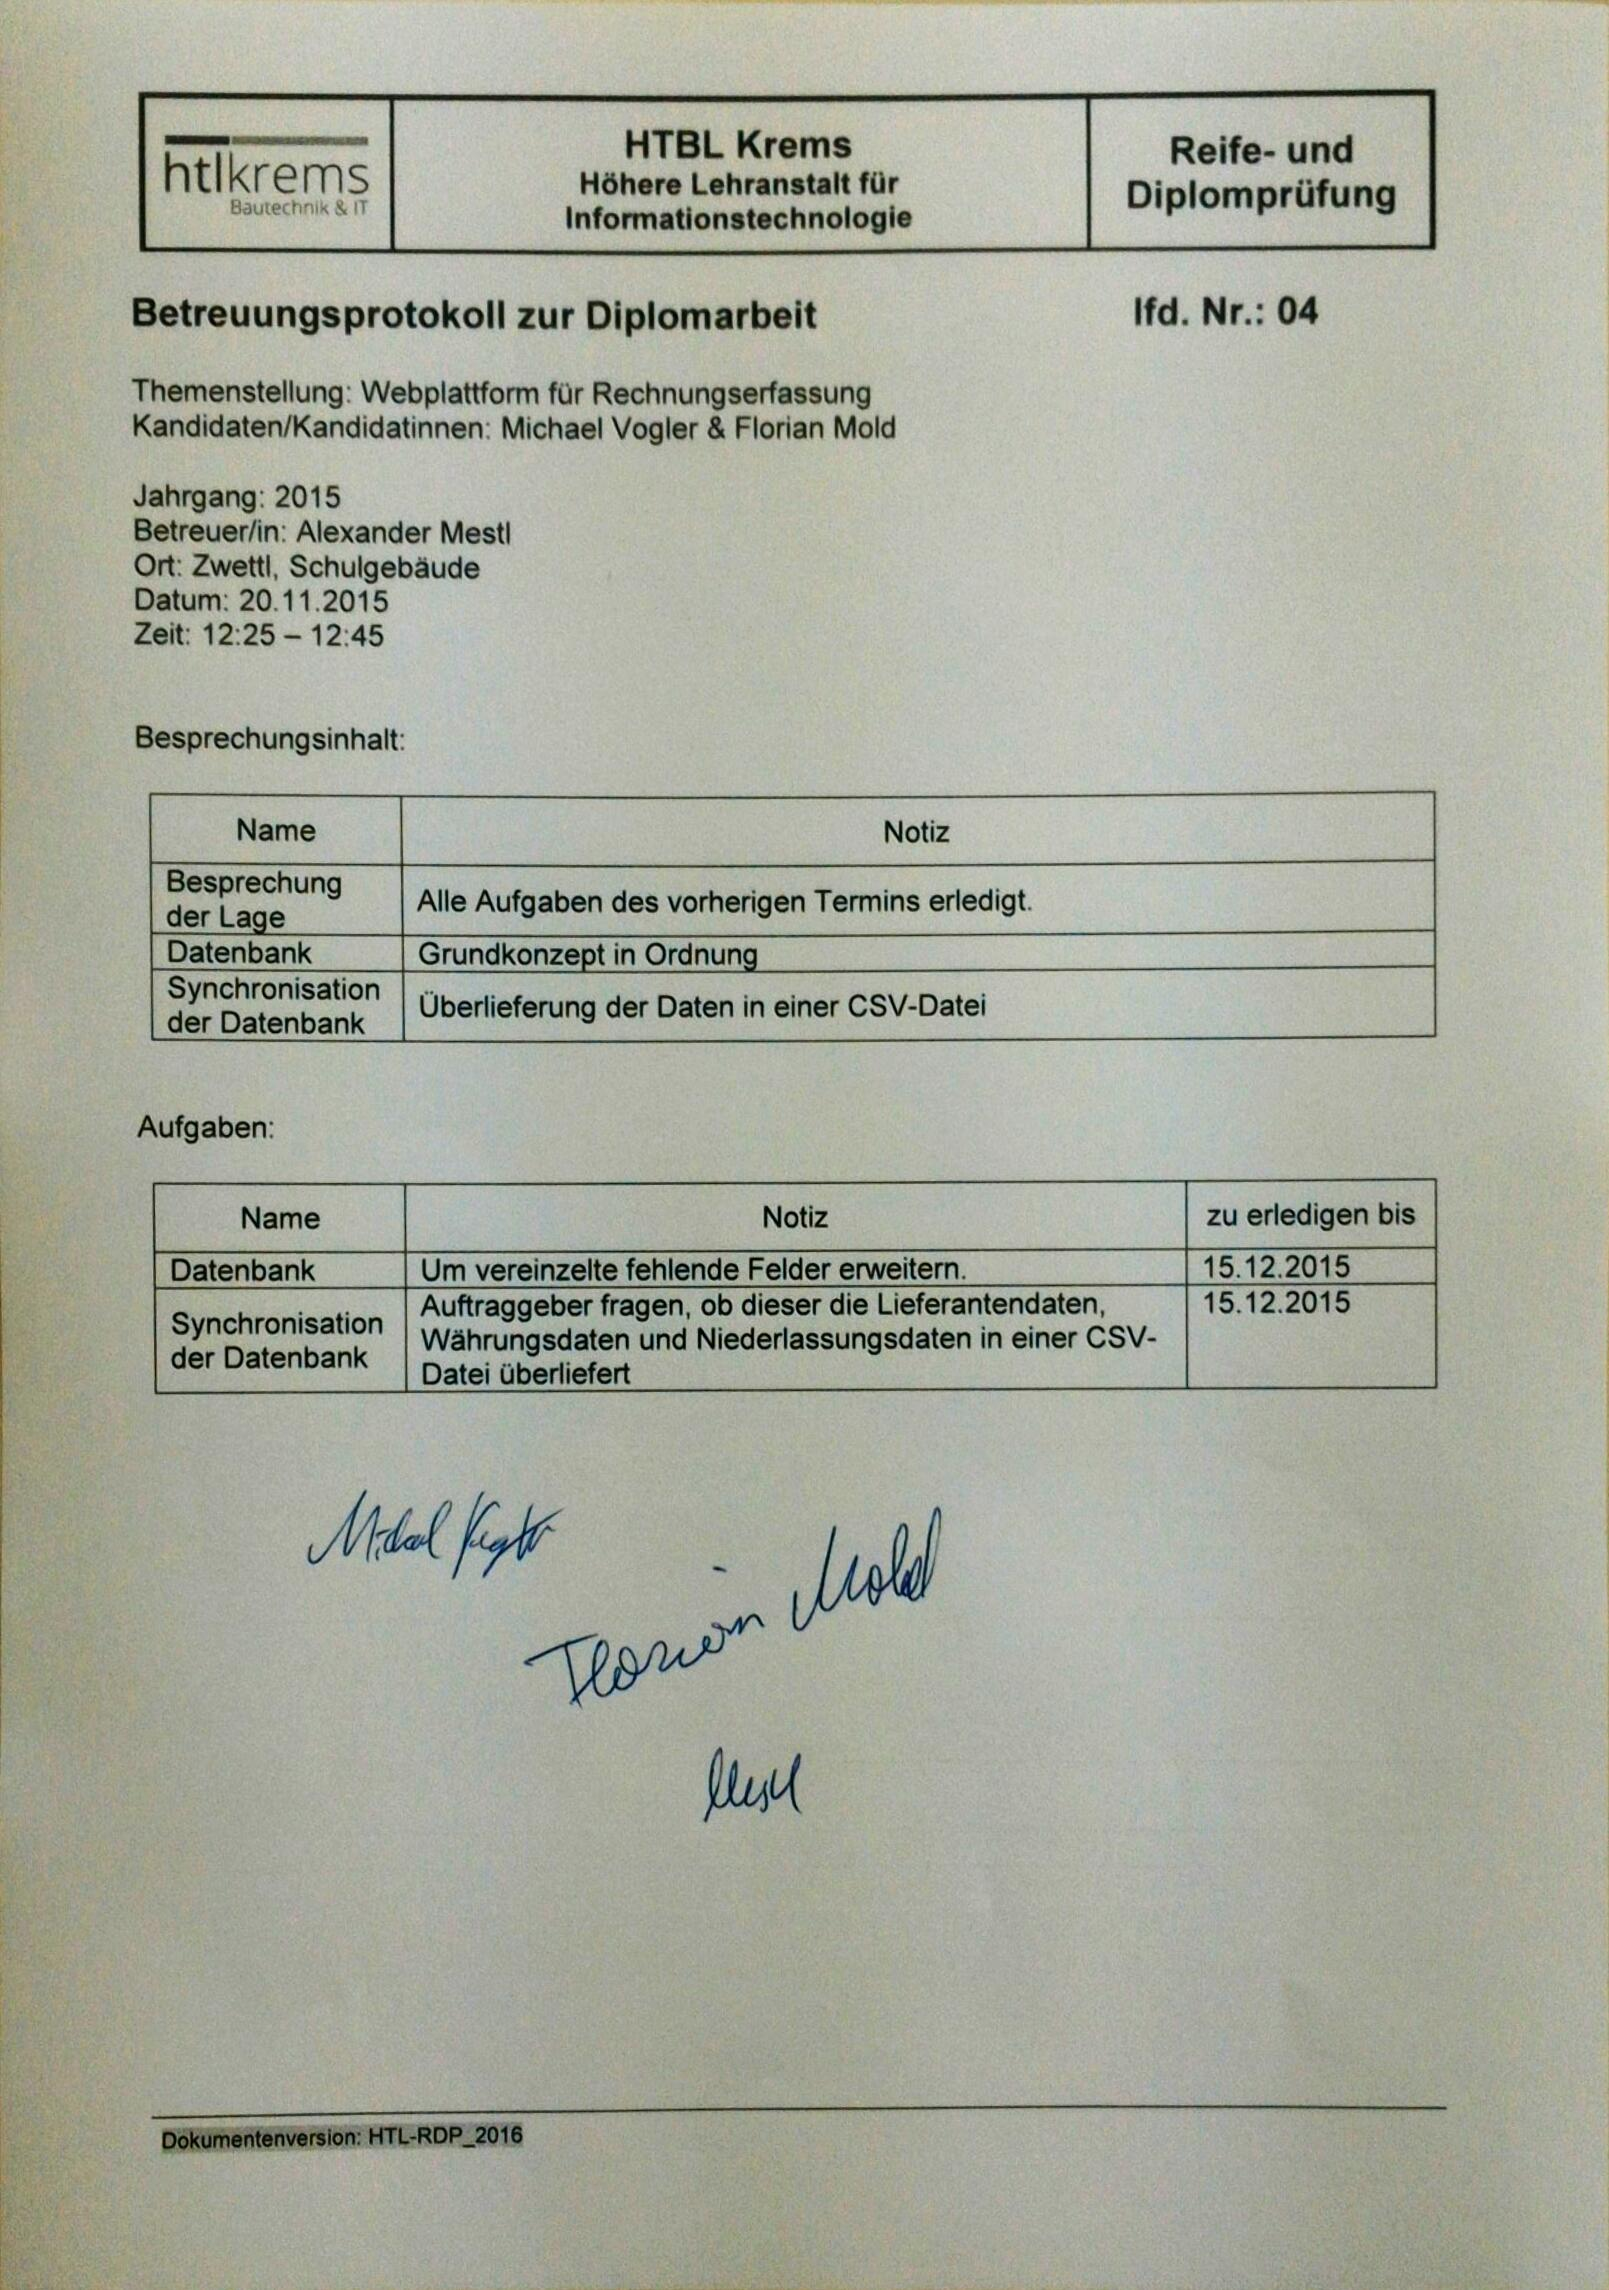
\includegraphics[width=13cm]{figures/Mestl_04.jpg}
    \label{fig:04_Protokoll_Betreuungslehrer}
    \caption{04 Protokoll mit Betreuungslehrer}
\end{figure}
\newpage
\begin{figure}[!h]
    \centering
    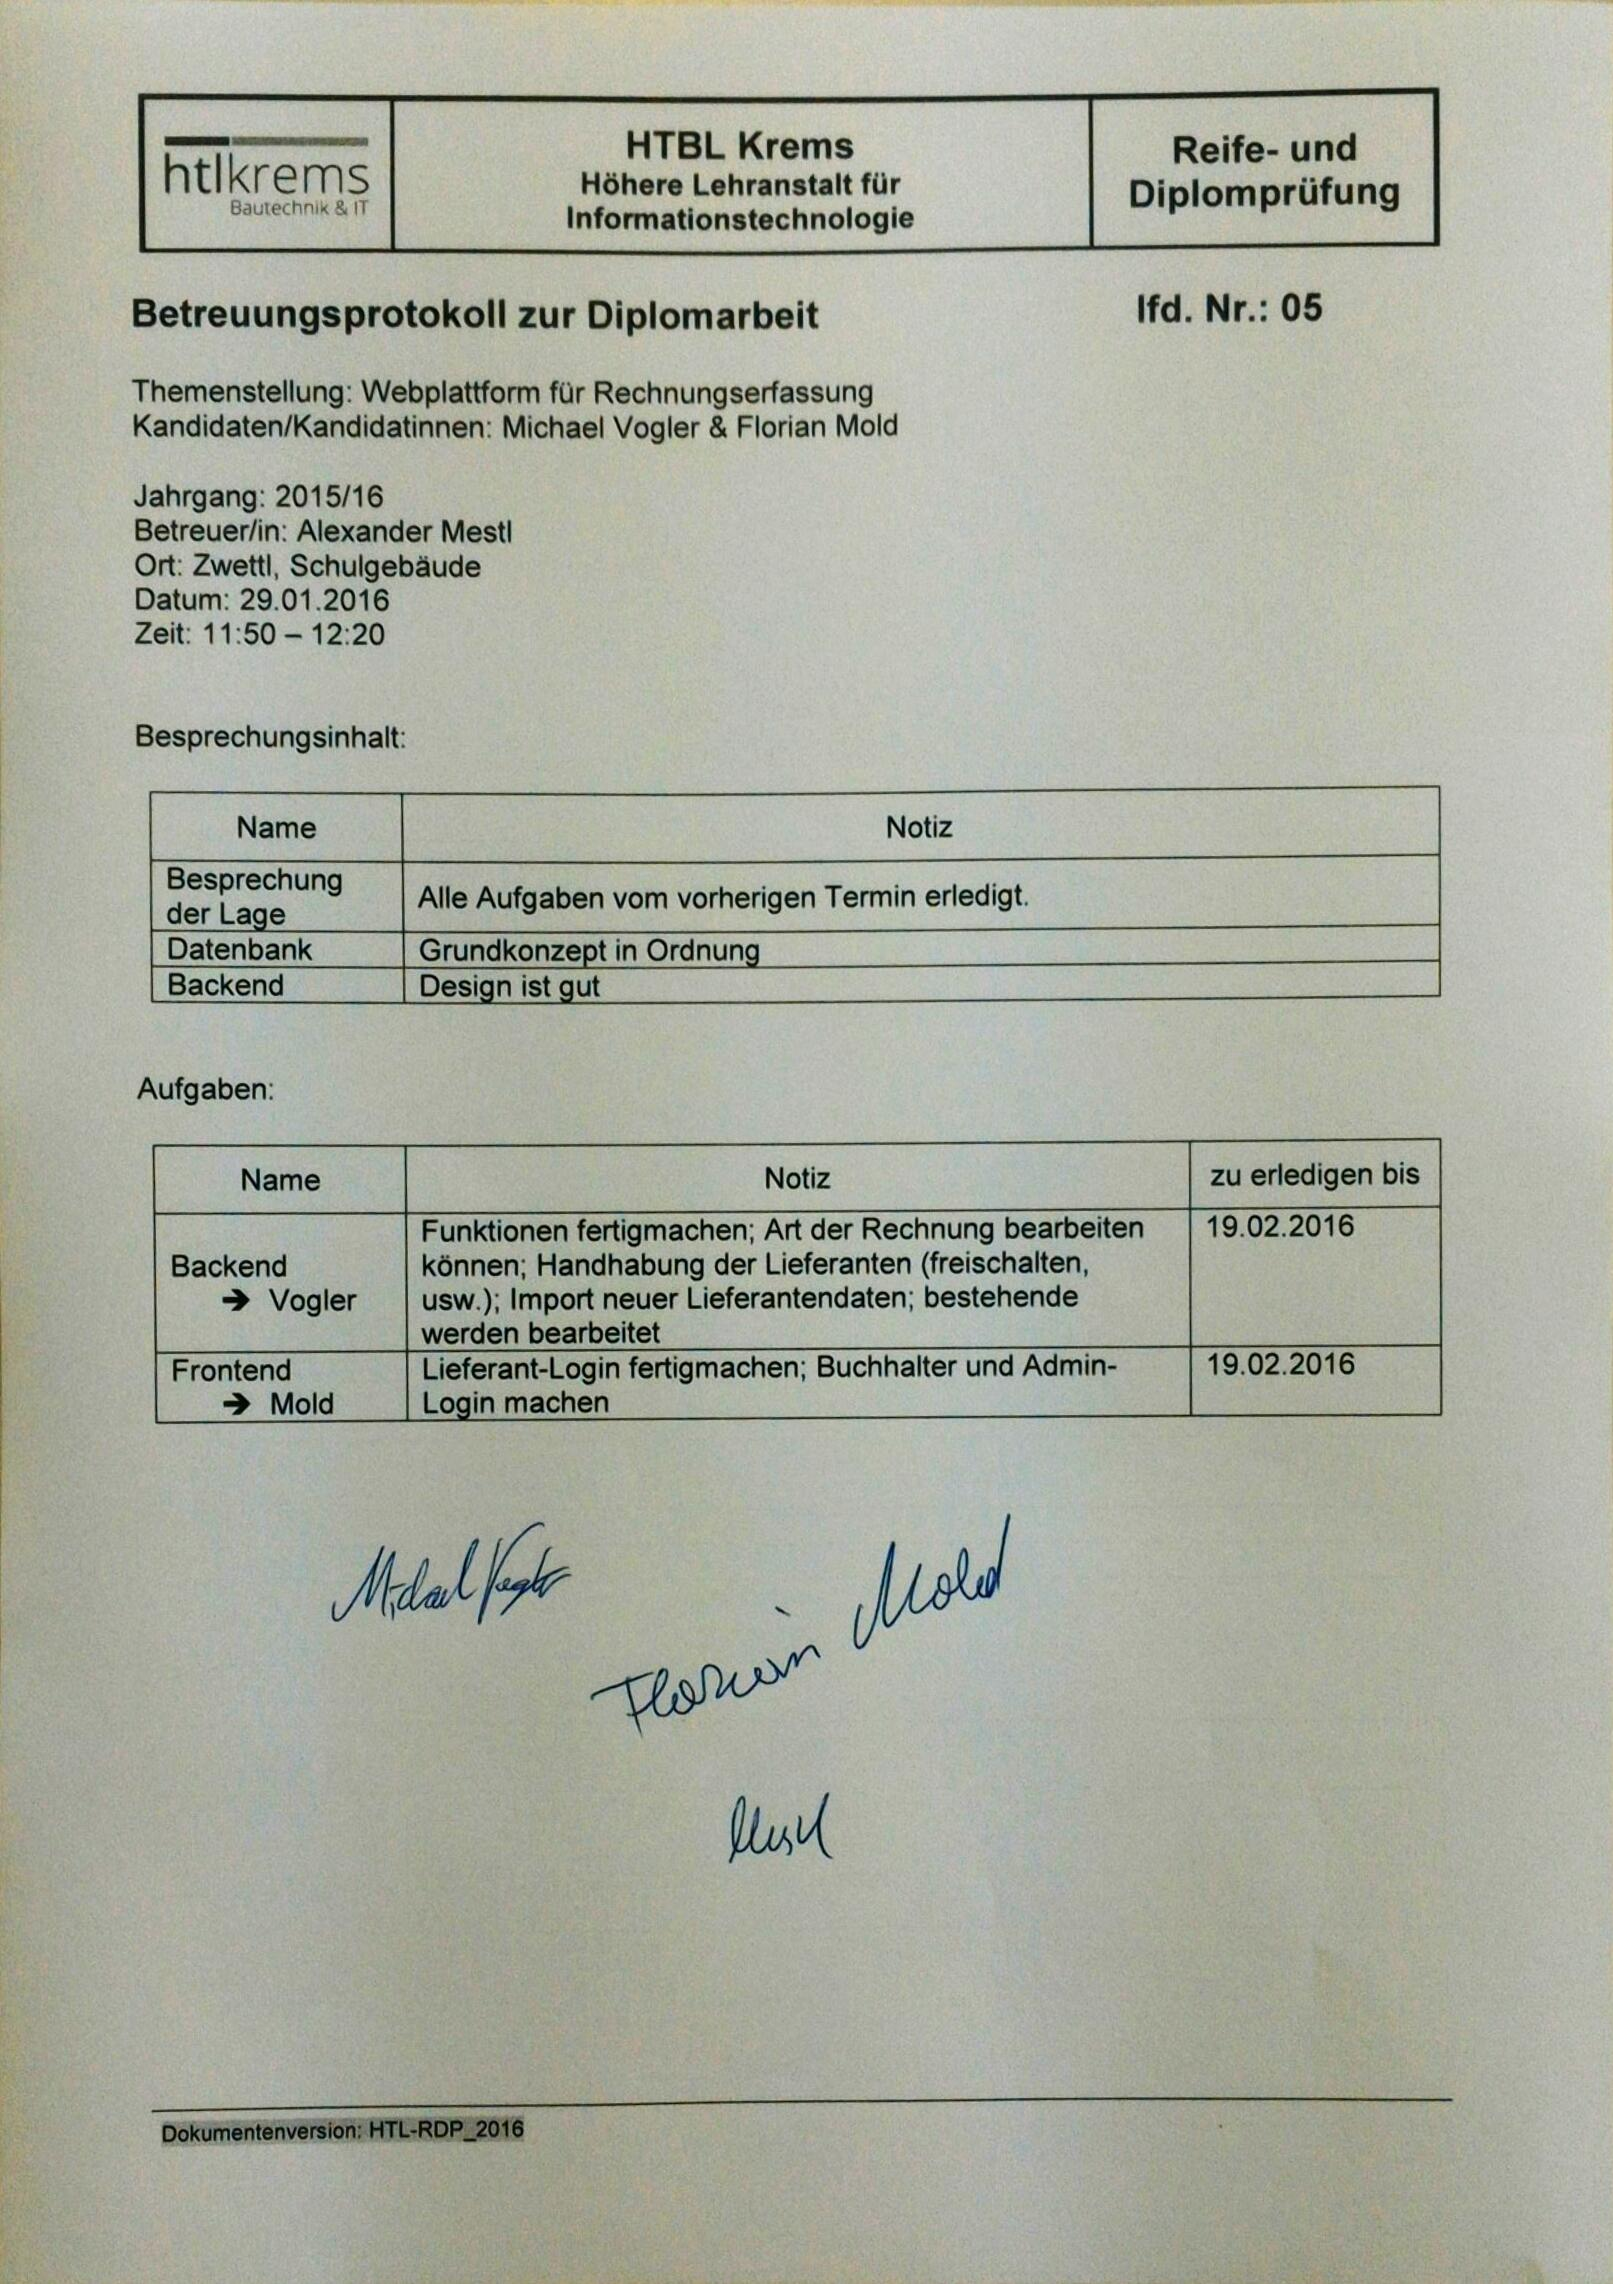
\includegraphics[width=13cm]{figures/Mestl_05.jpg}
    \label{fig:05_Protokoll_Betreuungslehrer}
    \caption{05 Protokoll mit Betreuungslehrer}
\end{figure}
\newpage
\begin{figure}[!h]
    \centering
    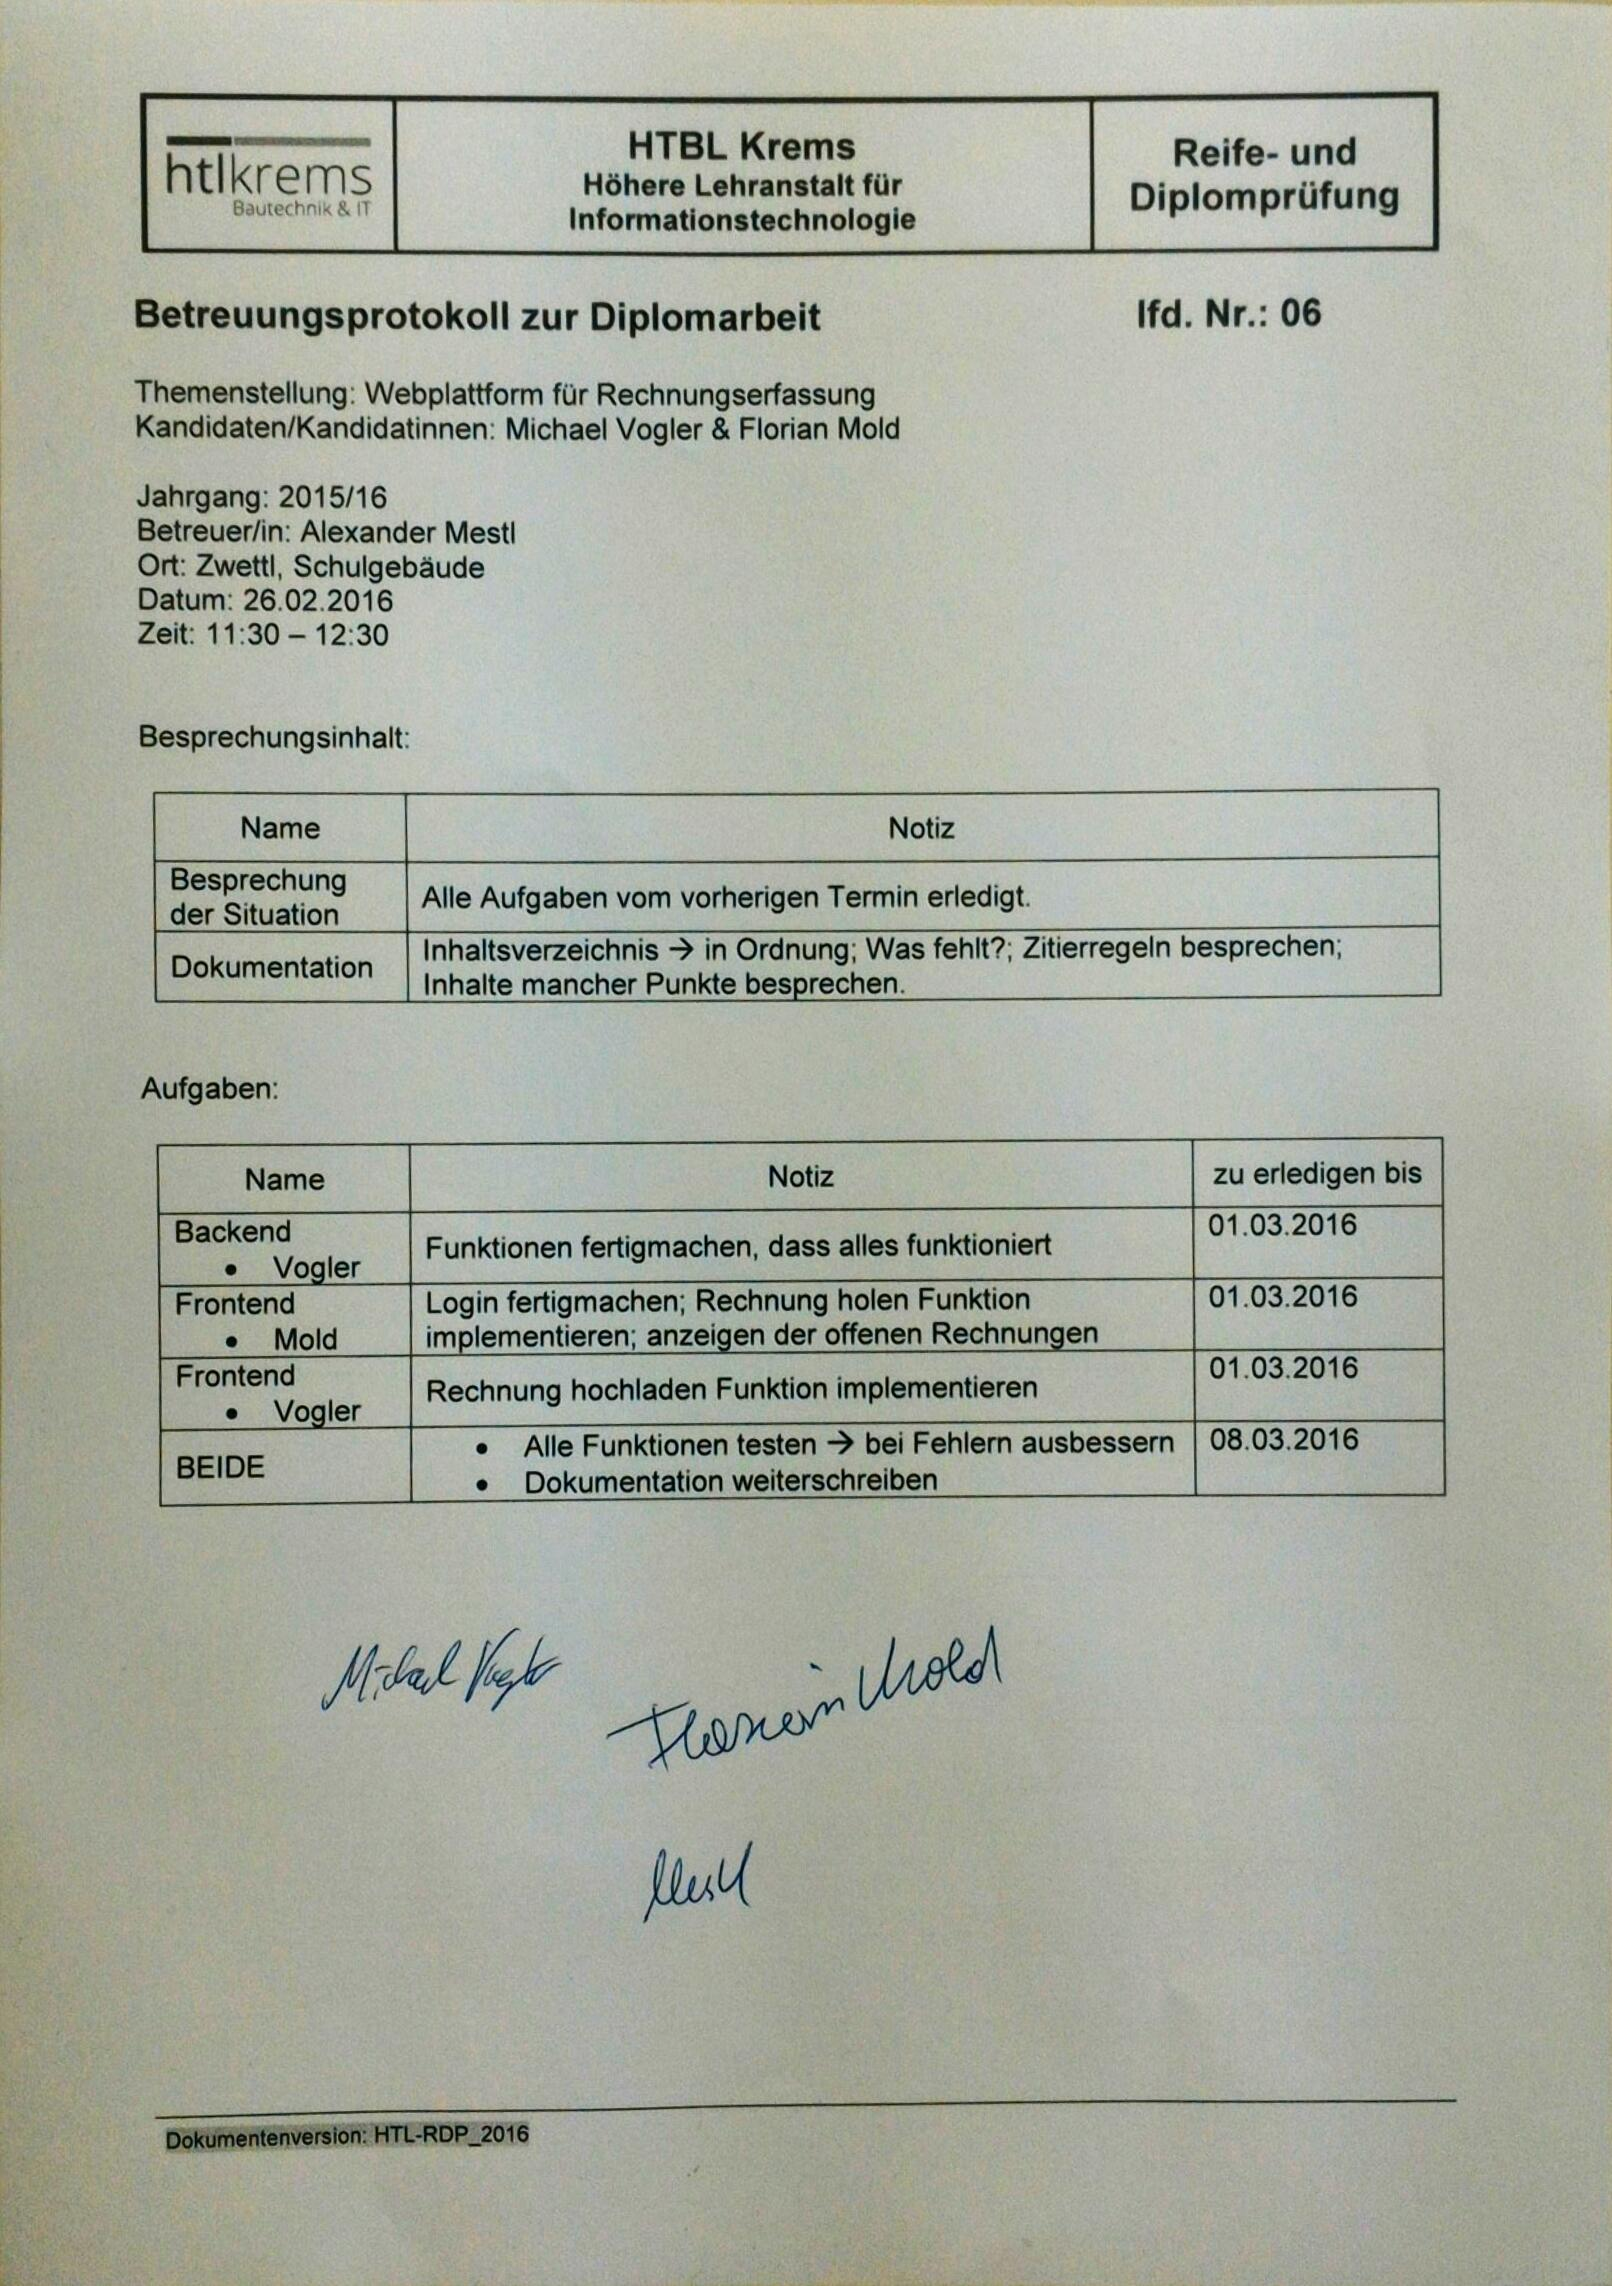
\includegraphics[width=13cm]{figures/Mestl_06.jpg}
    \label{fig:06_Protokoll_Betreuungslehrer}
    \caption{06 Protokoll mit Betreuungslehrer}
\end{figure}
\newpage


\section{Protokolle mit Ansprechpartner Herrn Ferkl}
Hier folgen alle Protokolle, von den einzelnen Besprechungen, die mit Herrn Ferkl durchgeführt wurden. Auf den Protokollen ist ersichtlich, wann und wo die Besprechung durchgeführt wurde, wer anwesend war und welche Inhalte wir besprochen haben.
\begin{figure}[!h]
    \centering
    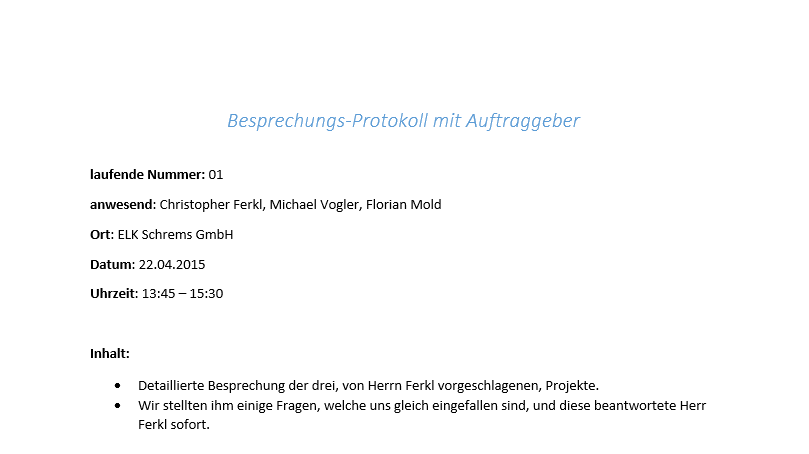
\includegraphics[width=16cm]{figures/Ferkl_01.png}
    \label{fig:01_Protokoll_Ansprechpartner}
    \caption{01 Protokoll mit Ansprechpartner}
\end{figure}

\begin{figure}[!h]
    \centering
    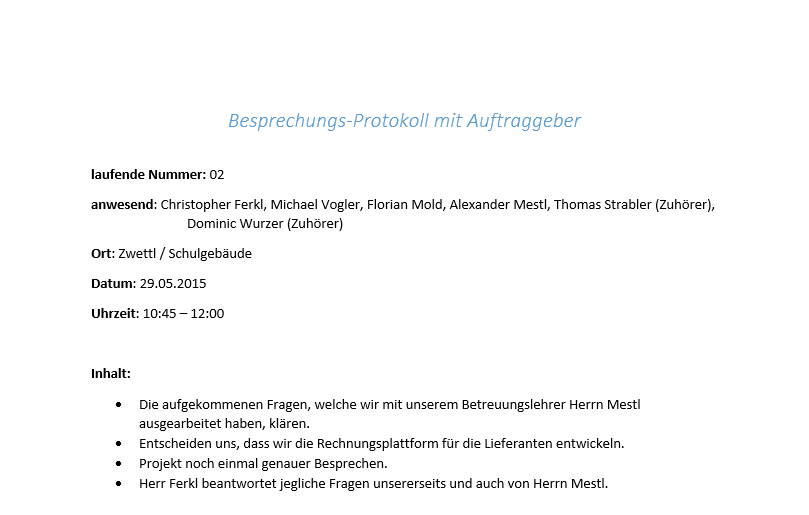
\includegraphics[width=16cm]{figures/Ferkl_02.png}
    \label{fig:02_Protokoll_Ansprechpartner}
    \caption{02 Protokoll mit Ansprechpartner}
\end{figure}
\newpage

\begin{figure}[!h]
    \centering
    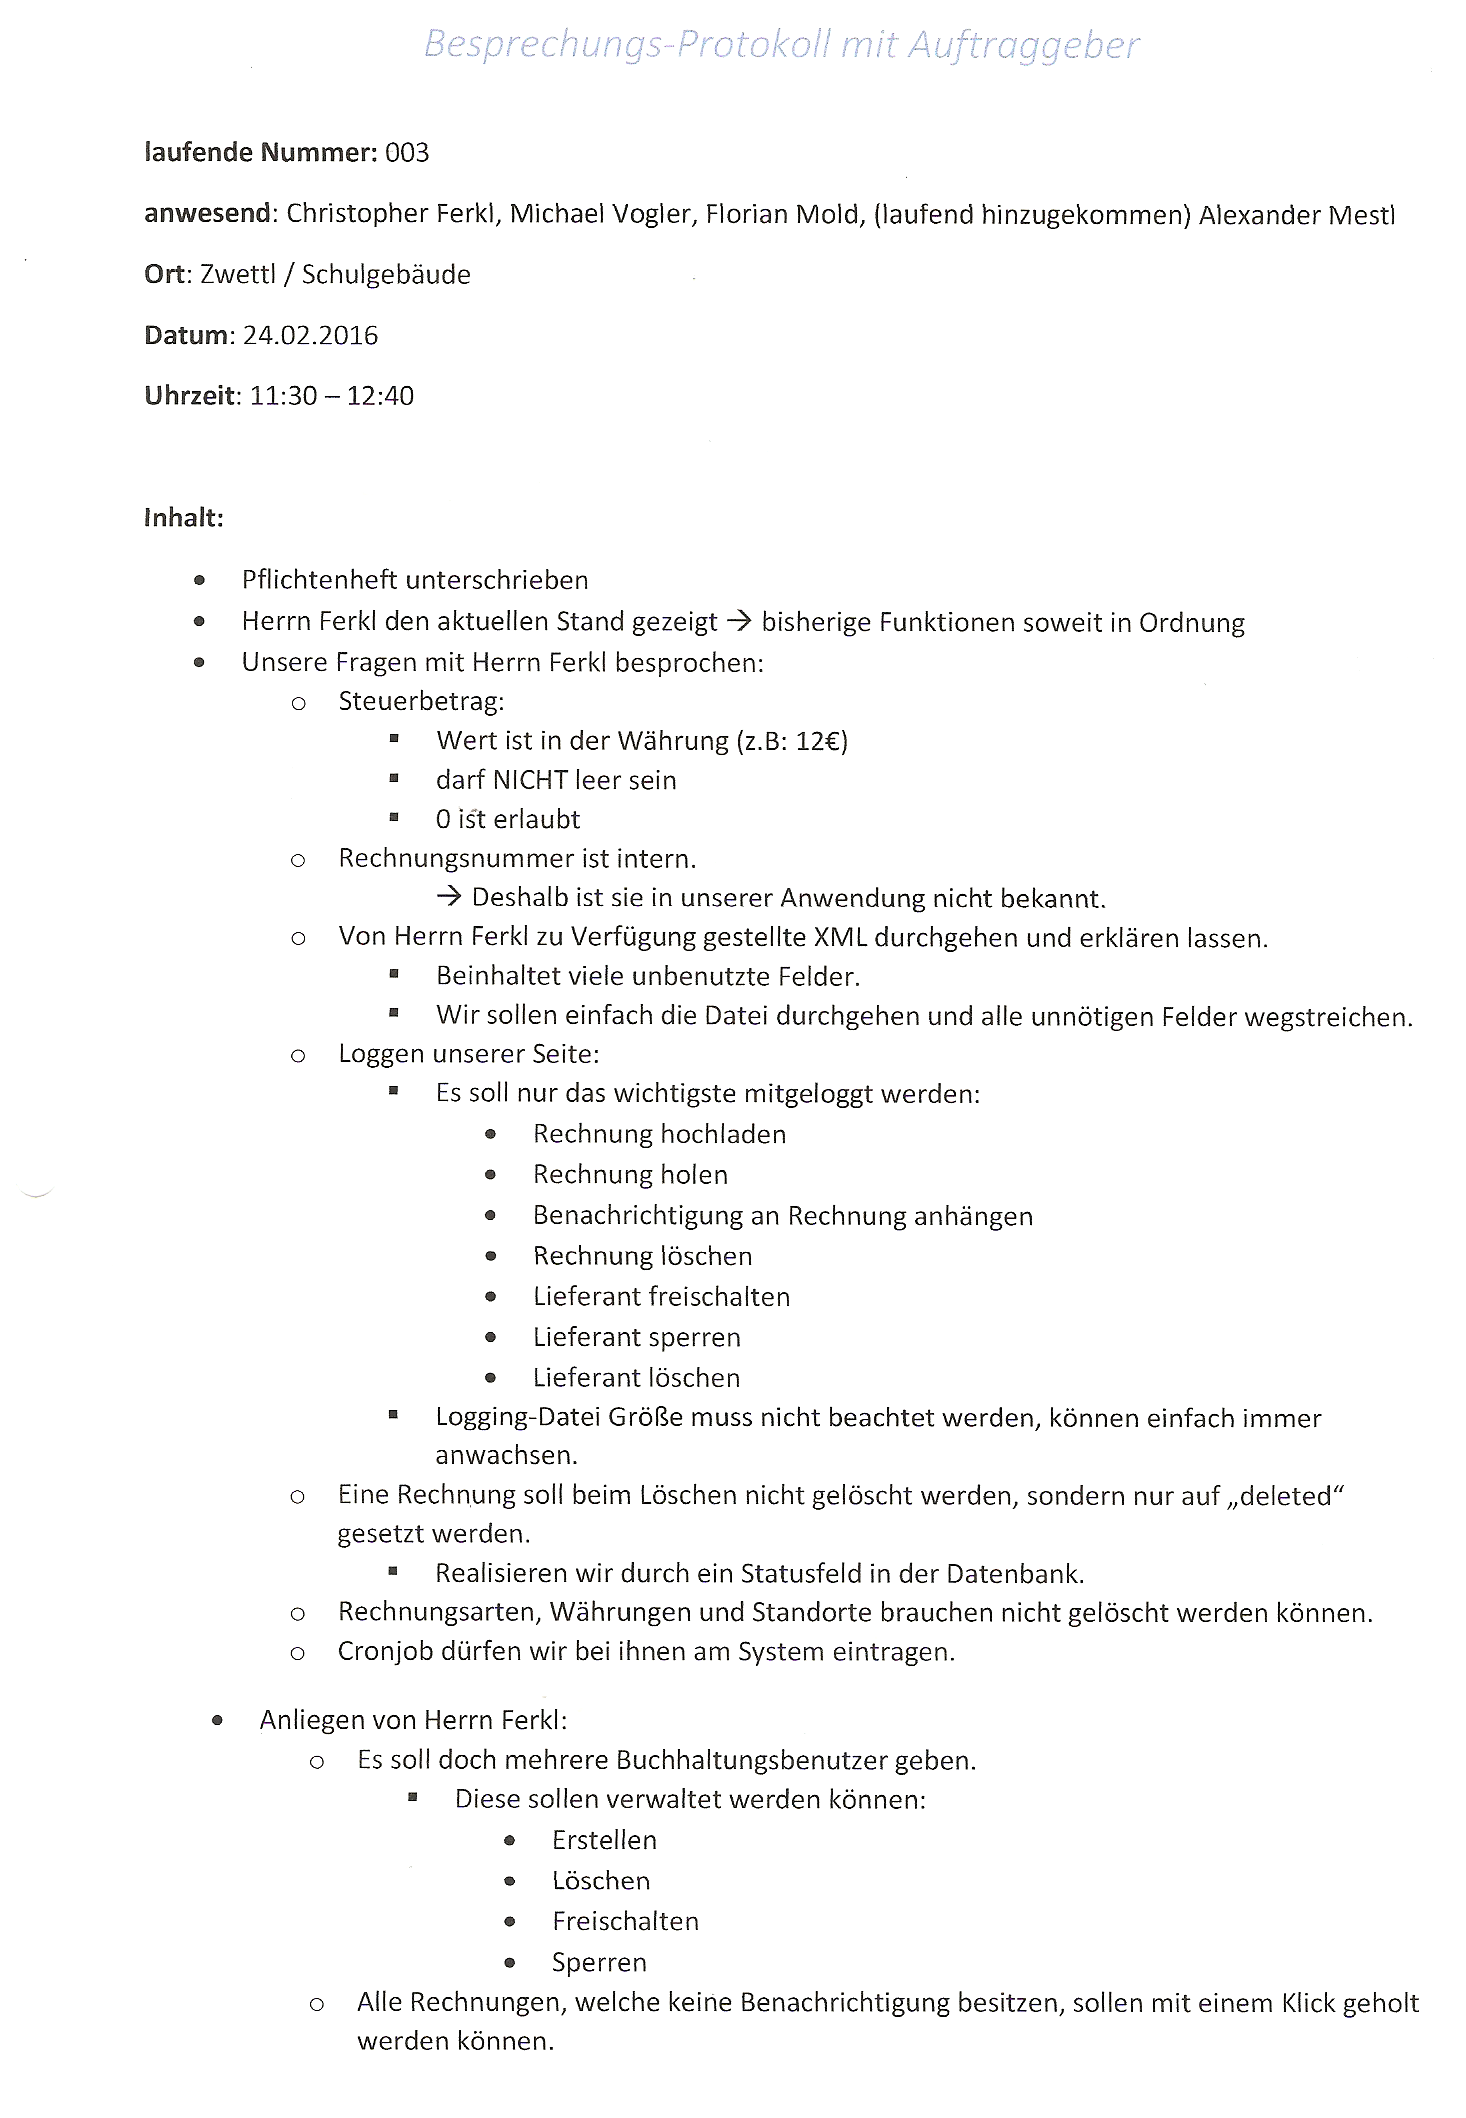
\includegraphics[width=16cm]{figures/Ferkl_03_1.png}
    \label{fig:03_Seite 1_Protokoll_Ansprechpartner}
    \caption{03 Seite 1 Protokoll mit Ansprechpartner}
\end{figure}
\end{appendix} 
\end{document}
d{appendix} 
\end{document}
ocument}
